%  LaTeX support: latex@mdpi.com 
%  For support, please attach all files needed for compiling as well as the log file, and specify your operating system, LaTeX version, and LaTeX editor.

%=================================================================
\documentclass[journal,article,submit,pdftex,moreauthors]{Definitions/mdpi} 
% For posting an early version of this manuscript as a preprint, you may use "preprints" as the journal and change "submit" to "accept". The document class line would be, e.g., \documentclass[preprints,article,accept,moreauthors,pdftex]{mdpi}. This is especially recommended for submission to arXiv, where line numbers should be removed before posting. For preprints.org, the editorial staff will make this change immediately prior to posting.

%--------------------
% Class Options:
%--------------------
%----------
% journal
%----------
% Choose between the following MDPI journals:
% acoustics, actuators, addictions, admsci, adolescents, aerospace, agriculture, agriengineering, agronomy, ai, algorithms, allergies, alloys, analytica, animals, antibiotics, antibodies, antioxidants, applbiosci, appliedchem, appliedmath, applmech, applmicrobiol, applnano, applsci, aquacj, architecture, arts, asc, asi, astronomy, atmosphere, atoms, audiolres, automation, axioms, bacteria, batteries, bdcc, behavsci, beverages, biochem, bioengineering, biologics, biology, biomass, biomechanics, biomed, biomedicines, biomedinformatics, biomimetics, biomolecules, biophysica, biosensors, biotech, birds, bloods, blsf, brainsci, breath, buildings, businesses, cancers, carbon, cardiogenetics, catalysts, cells, ceramics, challenges, chemengineering, chemistry, chemosensors, chemproc, children, chips, cimb, civileng, cleantechnol, climate, clinpract, clockssleep, cmd, coasts, coatings, colloids, colorants, commodities, compounds, computation, computers, condensedmatter, conservation, constrmater, cosmetics, covid, crops, cryptography, crystals, csmf, ctn, curroncol, currophthalmol, cyber, dairy, data, dentistry, dermato, dermatopathology, designs, diabetology, diagnostics, dietetics, digital, disabilities, diseases, diversity, dna, drones, dynamics, earth, ebj, ecologies, econometrics, economies, education, ejihpe, electricity, electrochem, electronicmat, electronics, encyclopedia, endocrines, energies, eng, engproc, ent, entomology, entropy, environments, environsciproc, epidemiologia, epigenomes, est, fermentation, fibers, fintech, fire, fishes, fluids, foods, forecasting, forensicsci, forests, foundations, fractalfract, fuels, futureinternet, futureparasites, futurepharmacol, futurephys, futuretransp, galaxies, games, gases, gastroent, gastrointestdisord, gels, genealogy, genes, geographies, geohazards, geomatics, geosciences, geotechnics, geriatrics, hazardousmatters, healthcare, hearts, hemato, heritage, highthroughput, histories, horticulturae, humanities, humans, hydrobiology, hydrogen, hydrology, hygiene, idr, ijerph, ijfs, ijgi, ijms, ijns, ijtm, ijtpp, immuno, informatics, information, infrastructures, inorganics, insects, instruments, inventions, iot, j, jal, jcdd, jcm, jcp, jcs, jdb, jeta, jfb, jfmk, jimaging, jintelligence, jlpea, jmmp, jmp, jmse, jne, jnt, jof, joitmc, jor, journalmedia, jox, jpm, jrfm, jsan, jtaer, jzbg, kidney, kidneydial, knowledge, land, languages, laws, life, liquids, literature, livers, logics, logistics, lubricants, lymphatics, machines, macromol, magnetism, magnetochemistry, make, marinedrugs, materials, materproc, mathematics, mca, measurements, medicina, medicines, medsci, membranes, merits, metabolites, metals, meteorology, methane, metrology, micro, microarrays, microbiolres, micromachines, microorganisms, microplastics, minerals, mining, modelling, molbank, molecules, mps, msf, mti, muscles, nanoenergyadv, nanomanufacturing, nanomaterials, ncrna, network, neuroglia, neurolint, neurosci, nitrogen, notspecified, nri, nursrep, nutraceuticals, nutrients, obesities, oceans, ohbm, onco, oncopathology, optics, oral, organics, organoids, osteology, oxygen, parasites, parasitologia, particles, pathogens, pathophysiology, pediatrrep, pharmaceuticals, pharmaceutics, pharmacoepidemiology, pharmacy, philosophies, photochem, photonics, phycology, physchem, physics, physiologia, plants, plasma, pollutants, polymers, polysaccharides, poultry, powders, preprints, proceedings, processes, prosthesis, proteomes, psf, psych, psychiatryint, psychoactives, publications, quantumrep, quaternary, qubs, radiation, reactions, recycling, regeneration, religions, remotesensing, reports, reprodmed, resources, rheumato, risks, robotics, ruminants, safety, sci, scipharm, seeds, sensors, separations, sexes, signals, sinusitis, skins, smartcities, sna, societies, socsci, software, soilsystems, solar, solids, sports, standards, stats, stresses, surfaces, surgeries, suschem, sustainability, symmetry, synbio, systems, taxonomy, technologies, telecom, test, textiles, thalassrep, thermo, tomography, tourismhosp, toxics, toxins, transplantology, transportation, traumacare, traumas, tropicalmed, universe, urbansci, uro, vaccines, vehicles, venereology, vetsci, vibration, viruses, vision, waste, water, wem, wevj, wind, women, world, youth, zoonoticdis 

%---------
% article
%---------
% The default type of manuscript is "article", but can be replaced by: 
% abstract, addendum, article, book, bookreview, briefreport, casereport, comment, commentary, communication, conferenceproceedings, correction, conferencereport, entry, expressionofconcern, extendedabstract, datadescriptor, editorial, essay, erratum, hypothesis, interestingimage, obituary, opinion, projectreport, reply, retraction, review, perspective, protocol, shortnote, studyprotocol, systematicreview, supfile, technicalnote, viewpoint, guidelines, registeredreport, tutorial
% supfile = supplementary materials

%----------
% submit
%----------
% The class option "submit" will be changed to "accept" by the Editorial Office when the paper is accepted. This will only make changes to the frontpage (e.g., the logo of the journal will get visible), the headings, and the copyright information. Also, line numbering will be removed. Journal info and pagination for accepted papers will also be assigned by the Editorial Office.

%------------------
% moreauthors
%------------------
% If there is only one author the class option oneauthor should be used. Otherwise use the class option moreauthors.

%---------
% pdftex
%---------
% The option pdftex is for use with pdfLaTeX. If eps figures are used, remove the option pdftex and use LaTeX and dvi2pdf.

%=================================================================
% MDPI internal commands
\firstpage{1} 
\makeatletter 
\setcounter{page}{\@firstpage} 
\makeatother
\pubvolume{1}
\issuenum{1}
\articlenumber{0}
\pubyear{2022}
\copyrightyear{2022}
%\externaleditor{Academic Editor: Firstname Lastname}
\datereceived{} 
%\daterevised{} % Only for the journal Acoustics
\dateaccepted{} 
\datepublished{} 
%\datecorrected{} % Corrected papers include a "Corrected: XXX" date in the original paper.
%\dateretracted{} % Corrected papers include a "Retracted: XXX" date in the original paper.
\hreflink{https://doi.org/} % If needed use \linebreak
%\doinum{}
%------------------------------------------------------------------
% The following line should be uncommented if the LaTeX file is uploaded to arXiv.org
%\pdfoutput=1

%=================================================================
% Add packages and commands here. The following packages are loaded in our class file: fontenc, inputenc, calc, indentfirst, fancyhdr, graphicx, epstopdf, lastpage, ifthen, lineno, float, amsmath, setspace, enumitem, mathpazo, booktabs, titlesec, etoolbox, tabto, xcolor, soul, multirow, microtype, tikz, totcount, changepage, attrib, upgreek, cleveref, amsthm, hyphenat, natbib, hyperref, footmisc, url, geometry, newfloat, caption
% \usepackage{cite}
\usepackage{picinpar}
\usepackage{flushend}
% \usepackage[latin1]{inputenc}
\usepackage{colortbl}
\usepackage{pifont}
\usepackage{color}
\usepackage{alltt}
% \usepackage[hidelinks]{hyperref}
% \usepackage{enumerate}
\usepackage{siunitx}
\usepackage{breakurl}
\usepackage{pbox}

% Adds SVG Support out of SVG file
\usepackage{svg}
% \svgsetup{inkscape=force}   % Rerenders the inkscape images with new variants
% \svgsetup{inkscape=page}

% Fancy table related trick
\usepackage{makecell}
\def\chk{\tikz\fill[scale=0.4](0,.35) -- (.25,0) -- (1,.7) -- (.25,.15) -- cycle;}

% Python code
\usepackage{listings}
%Code listing style
\lstdefinestyle{mystyle}{
  backgroundcolor=\color{backcolour},   commentstyle=\color{codegreen},
  keywordstyle=\color{magenta},
  numberstyle=\tiny\color{codegray},
  stringstyle=\color{codepurple},
  basicstyle=\ttfamily\footnotesize,
  breakatwhitespace=false,         
  breaklines=true,                 
  captionpos=b,                    
  keepspaces=true,                 
  numbers=left,                    
  numbersep=5pt,                  
  showspaces=false,                
  showstringspaces=false,
  showtabs=false,                  
  tabsize=2
}

%style code listing set
\lstset{style=mystyle}

% Algorithmic
\usepackage{algorithm, algorithmic}

% Subfigures
\usepackage{subcaption}

% Produce landscape pages in a (mainly) portrait document.
% \usepackage{pdflscape}

% Adding if execution to define between thesis and article
\newboolean{thesis}
\setboolean{thesis}{false}

% Intext plus-minus
\usepackage{textcomp}

%New colors defined below
\definecolor{codegreen}{rgb}{0,0.6,0}
\definecolor{codegray}{rgb}{0.5,0.5,0.5}
\definecolor{codepurple}{rgb}{0.58,0,0.82}
\definecolor{backcolour}{rgb}{0.95,0.95,0.92}
\definecolor{limegreen}{rgb}{0.2, 0.8, 0.2}
\definecolor{forestgreen}{rgb}{0.13, 0.55, 0.13}
\definecolor{greenhtml}{rgb}{0.0, 0.5, 0.0}
%=================================================================
%% Please use the following mathematics environments: Theorem, Lemma, Corollary, Proposition, Characterization, Property, Problem, Example, ExamplesandDefinitions, Hypothesis, Remark, Definition, Notation, Assumption
%% For proofs, please use the proof environment (the amsthm package is loaded by the MDPI class).

%=================================================================
% Full title of the paper (Capitalized)
\Title{Practical evaluation of Lithium-Ion battery State of Charge estimation using Time-Series Machine Learning for Electric Vehicles}

% MDPI internal command: Title for citation in the left column
\TitleCitation{Practical evaluation of Lithium-Ion battery State of Charge estimation using Time-Series Machine Learning for Electric Vehicles}

% Author Orchid ID: enter ID or remove command
\newcommand{\orcidauthorA}{0000-0000-0000-000X} % Add \orcidA{} behind the author's name
\newcommand{\orcidauthorB}{0000-0000-0000-000X} % Add \orcidB{} behind the author's name
\newcommand{\orcidauthorC}{0000-0000-0000-000X} % Add \orcidB{} behind the author's name
\newcommand{\orcidauthorD}{0000-0000-0000-000X} % Add \orcidB{} behind the author's name

% Authors, for the paper (add full first names)
\Author{Marat Sadykov $^{1,\ddagger}$\orcidA{}, Sam Haines, Dr Mark Broadmeadow\orcidD{}, A/Prof Geoff Walker\orcidC{} and A/Prof David Holmes $^{2,\dagger,\ddagger}$*\orcidB{}}

%\longauthorlist{yes}

% MDPI internal command: Authors, for metadata in PDF
\AuthorNames{Marat Sadykov, Sam Haines, Dr Mark Broadmeadow, A/Prof Geoff Walker and A/Prof David Holmes}

% MDPI internal command: Authors, for citation in the left column
%! Verify the order for principal superviosors
\AuthorCitation{Sadykov, M.; Holmes, D.; Haines, S.; Broadmeadow, M.; Walker, G.}
% If this is a Chicago style journal: Lastname, Firstname, Firstname Lastname, and Firstname Lastname.

% Affiliations / Addresses (Add [1] after \address if there is only one affiliation.)
\address{%
$^{1}$ \quad Affiliation 1; e-mail@e-mail.com\\
$^{2}$ \quad Affiliation 2; e-mail@e-mail.com}

% Contact information of the corresponding author
\corres{Correspondence: e-mail@e-mail.com; Tel.: (optional; include country code; if there are multiple corresponding authors, add author initials) +xx-xxxx-xxx-xxxx (F.L.)}

% Current address and/or shared authorship
\firstnote{Current address: Affiliation 3.} 
\secondnote{These authors contributed equally to this work.}
% The commands \thirdnote{} till \eighthnote{} are available for further notes

%\simplesumm{} % Simple summary

%\conference{} % An extended version of a conference paper

% Abstract (Do not insert blank lines, i.e. \\) 
\abstract{
	% State of Charge (SoC) estimation is a crucial property of a Lithium-Ion battery in any electrical system.
	% An accurate charge percentage, without any discrepancies, allows a battery management system (BMS) to enhance battery module utilisation further, allowing higher endurance or prolonging overall utilisation for more cycles.
	% There have been numerous attempts to determine SoC without physical intervention, such as battery modelling.
	% Since batteries commonly have non-linear characteristics, statistical-based Machine Learning methods have the potential to replace the traditional model.
	The present paper conducts a practical usability investigation on Recurrent Neural Networks (RNN) to determine the best-suited machine learning method for Electric vehicles (EV).
	Through the implementation of models from multiple published sources and cross-validation testing with several driving scenarios of Lithium-Ion batteries, several models have been assessed on accuracy and drawbacks.% against simulations of different driving conditions.
	% \begin{itemize}
	%     \item Five models were selected from various published State of Charge estimation models based on cell types (GRU and LSTM with Attention) and optimisers (SGD, Adam, Nadam, AdaMax and Robust Adam).
	%     \item Five models were selected from various published State of Charge estimation models based on cell types of GRU or LSTM and optimisers like Stochastic Gradient Descent, Adam, Nadam, AdaMax and Robust Adam, with extensions via Momentum calculus or Attention layer.
	% \end{itemize}
	Five models were selected from various published State of Charge estimation models based on cell types of GRU or LSTM and optimisers like Stochastic Gradient Descent, Adam, Nadam, AdaMax and Robust Adam, with extensions via Momentum calculus or Attention layer.
	Each method will be examined by applying training techniques like a learning rate scheduler or rollback recovery to speed up fitting, highlighting implementation specifics, and all of that using the TensorFlow framework as close as possible to the published sources on openly available battery data.
	The results highlight the percentage accuracy in the average of 3.64\% of Root Mean Squared Error, several drawbacks of the overall implementation, and propose potential solutions for further improvement.
	Every implemented model had a similar drawback of poor capturing of the middle area of a charge, applying higher weight on a voltage rather than current.
	The combined techniques in a single custom model could be better suited to improve accuracy further.
}

% Keywords
\keyword{
    % Adaptive Moment Estimation (Adam);
    % Adaptive Moment Estimation based on the infinity norm (Adamax);
    % Attention Layer;
    % Chip-on-Board (CoB);
    Driving schedulers;
    % Electric Vehicle (EV);
    Gradient Recurrent Unit (GRU);
    Optimisers;
    Lithium-Ion battery (Li-Ion);
    Long Short-Term Memory (LSTM);
    % Nesterov Adaptive Moment Estimation (Nadam);
    % Raspberry Pi 4 (R-Pi4);
    Recurrent Neural Networks (RNNs);
    % Robust Online Adaptive Moment Estimation (RoAdam);
    State of Charge (SOC) estimation;
    % Stochastic Gradient Descent with Momentum (SGDw/M);
    % Tensor Processing Unit (TPU);
    % TensorFlow (TF);
    Time-Series Machine Learning
}

% The fields PACS, MSC, and JEL may be left empty or commented out if not applicable
%\PACS{J0101}
%\MSC{}
%\JEL{}

%%%%%%%%%%%%%%%%%%%%%%%%%%%%%%%%%%%%%%%%%%
% Only for the journal Diversity
%\LSID{\url{http://}}

%%%%%%%%%%%%%%%%%%%%%%%%%%%%%%%%%%%%%%%%%%
% Only for the journal Applied Sciences
%\featuredapplication{Authors are encouraged to provide a concise description of the specific application or a potential application of the work. This section is not mandatory.}
%%%%%%%%%%%%%%%%%%%%%%%%%%%%%%%%%%%%%%%%%%

%%%%%%%%%%%%%%%%%%%%%%%%%%%%%%%%%%%%%%%%%%
% Only for the journal Data
%\dataset{DOI number or link to the deposited data set if the data set is published separately. If the data set shall be published as a supplement to this paper, this field will be filled by the journal editors. In this case, please submit the data set as a supplement.}
%\datasetlicense{License under which the data set is made available (CC0, CC-BY, CC-BY-SA, CC-BY-NC, etc.)}

%%%%%%%%%%%%%%%%%%%%%%%%%%%%%%%%%%%%%%%%%%
% Only for the journal Toxins
%\keycontribution{The breakthroughs or highlights of the manuscript. Authors can write one or two sentences to describe the most important part of the paper.}

%%%%%%%%%%%%%%%%%%%%%%%%%%%%%%%%%%%%%%%%%%
% Only for the journal Encyclopedia
%\encyclopediadef{For entry manuscripts only: please provide a brief overview of the entry title instead of an abstract.}

%%%%%%%%%%%%%%%%%%%%%%%%%%%%%%%%%%%%%%%%%%
% Only for the journal Advances in Respiratory Medicine
%\addhighlights{yes}
%\renewcommand{\addhighlights}{%

%\noindent This is an obligatory section in “Advances in Respiratory Medicine”, whose goal is to increase the discoverability and readability of the article via search engines and other scholars. Highlights should not be a copy of the abstract, but a simple text allowing the reader to quickly and simplified find out what the article is about and what can be cited from it. Each of these parts should be devoted up to 2~bullet points.\vspace{3pt}\\
%\textbf{What are the main findings?}
% \begin{itemize}[labelsep=2.5mm,topsep=-3pt]
% \item First bullet.
% \item Second bullet.
% \end{itemize}\vspace{3pt}
%\textbf{What is the implication of the main finding?}
% \begin{itemize}[labelsep=2.5mm,topsep=-3pt]
% \item First bullet.
% \item Second bullet.
% \end{itemize}
%}

%%%%%%%%%%%%%%%%%%%%%%%%%%%%%%%%%%%%%%%%%%
\begin{document}
%%%%%%%%%%%%%%%%%%%%%%%%%%%%%%%%%%%%%%%%%%
%%% Introduction
\section{Introduction} \label{sec:Introduction}
\IEEEPARstart{T}{he} market for Electrical Vehicles (EV) has grown significantly over the past decade~\cite{state-ev-australia}.
The replacement of a fossil fuel-based engine with an electric drivetrain eliminates exhaust emissions with the potential to reduce human impact on climate change significantly.
For EVs to grow market share and reduce costs, battery cost and longevity must be improved.
Extensive battery cycling leads to battery degradation over time (aging).
The development of smarter and more accurate battery management strategies may be capable of prolonging service duty.
This would rely upon a system's ability to estimate a battery's state at any point in time.
An accurate charge calculation avoids overcharging or over-discharging, leading to improved battery service utilisation, better health estimation, longer life span, more reliable range prediction and further benefits~\cite{calif_proper_2008}.

%
%
The development of effective methods for State-of-Charge (SoC) estimation remains a topic of crucial research focus.
Various techniques to estimate the SoC have been developed to enhance battery usage.
The ability to determine the state of a battery or a battery system is a required function for an advanced Battery Management System (BMS).
Those techniques can be classified into three primary categories~\cite{ali_towards_2019,ng_enhanced_2009,robust_SoC,6953745}: direct measurement, model-based methods, and computer intelligence or Machine Learning (ML).
Direct measurements methods take readings from batteries relying on sensors, such as open circuit Voltage, internal resistance, or current readings over set periods (i.e. Coulomb Counting)~\cite{ng_enhanced_2009,robust_SoC}.
Model-based methods recreate battery behaviour and use sensor inputs to calculate results from a pre-defined model~\cite{6953745}.
Computer intelligence techniques enhance such models with additional data.
Those data-driven calculations aim to improve model estimation by fitting to an actual behaviour observation.
Examples include Fuzzy Logic~\cite{malkhandi_fuzzy_2006}, Support Vector Machine~\cite{hansen_support_2005, anton_battery_2013}, or Neural Networks (NN)~\cite{song_lithium-ion_2018,Chemali2017,mamo_long_2020,jiao_gru-rnn_2020,xiao_accurate_2019,javid_adaptive_2020,zhang_deep_2020}.

%
%
While some model-based methods, such as the equivalent circuit model, are simple to implement within a BMS, many cannot correctly capture batteries' complex multi-dependant behaviour~\cite{6953745}.
%Others are limited to offline simulation due to high complexity and computation requirements, therefore not suited to an onboard BMS.
Direct measurement estimation is limited to sensor accuracy and affected by losses created by Coulombic efficiencies~\cite{Smith_2010} where some portion of charge gets transferred to heat or gets affected by battery ageing that is not captured.
%Additionally, the measured voltage depends on whether the battery is in use or has been on rest for a given time.
%An accurate SoC estimation model has to implement a way to accommodate battery losses and sensor readings.
%If model-based methods treat as constant values, then in real scenarios, they can be significantly limited to sensor inaccuracy, environmental and internal battery temperature, or aging.
%In contrast, Neural Network methods can accommodate losses as they can capture complex phenomenological behaviours~\cite{bengio_learning_1994}.
%
%Smart BMSs, which incorporate some method of ML, use only sensory data~\cite{zhang_deep_2020} and do not require a batteries physical property~\cite{zhang_deep_2020}.
In contrast, Machine Learning are known to be able to establish relationships in complicated and multi-dimensional non-linear systems~\cite{hansen_support_2005,anton_battery_2013,he_state_2014}.
This characteristic shows great potential to account for battery losses due to Coulumbic efficiency.
Some researchers used the support vector machine-based methods to estimate SoC using voltage, current, and temperature inputs~\cite{hansen_support_2005,anton_battery_2013}.
Data were obtained from a driving schedule profile on a battery cycler, and the end error estimation was achieved as less than 6\%~\cite{he_state_2014}.
%The solution to lowering that percentage may lie within the more complicated models, like Neural Networks.
Many attempts to implement different Neural Networks exist, but the most promising net for charge estimation were Recurrent Neural Networks (RNN)~\cite{song_lithium-ion_2018,Chemali2017,mamo_long_2020,jiao_gru-rnn_2020,xiao_accurate_2019,javid_adaptive_2020,zhang_deep_2020}.
Their effectiveness in time-series dependant problems was shown using internal neurons to process data sequences with varying lengths by Chemali et al.~\cite{Chemali2017}.
% The models' cells act as memory units, building relationships and giving outputs based on multiple inputs over time.
% Typical examples are data forecasting, handwriting, speech and image recognition, machine translation or music composition~\cite{devdarshan_applications_2019}. 

% 
%
Over the past years, the RNN approach has found multiple applications for SoC estimation.
The most recent attempt to determine the Li-Ion battery's remaining useful life was with implementation of the Gradient Recurrent Unit models~\cite{song_lithium-ion_2018,javid_adaptive_2020,xiao_accurate_2019,jiao_gru-rnn_2020}.
The earliest approach utilised a battery charge's regression nature only using stateless models~\cite{song_lithium-ion_2018,jiao_gru-rnn_2020,xiao_accurate_2019} when input impact is not preserved for further predictions.
Later, some approaches introduced additional parameters to support the NN learning process~\cite{mamo_long_2020,jiao_gru-rnn_2020,javid_adaptive_2020}.
Besides good convergences, the model's use was in determining critical events, like the time before complete charge depletion or overcharge.
However, it did not receive wide application due to its initial state requirement as input features.
The most popular way lies in determining the charge's value using a fixed size history of voltage, current, and temperature in stateless Long Short-Term Memory (LSTM) models~\cite{Chemali2017,mamo_long_2020,javid_adaptive_2020,zhang_deep_2020}.
The method's advantage is independent of the charge or discharge cycles at different times, as long as the history samples are in order.
However, estimation determines values based on fixed history samples and does not preserve for the next prediction, making practical estimation of single or several charge values, but not determining critical events ahead.
That can be achieved with stateful models, which continuously preserve the prediction's impact and can be propagated further until they reach the end state without resets~\cite{zhu_statefulnes_tfdocs_2020}.

%
%
One of the first attempts to train an RNN model to predict the state of charge is to train in several cycles of a single battery utilisation dataset at different temperatures~\cite{song_lithium-ion_2018, xiao_accurate_2019,javid_adaptive_2020, jiao_gru-rnn_2020}.
Then as others attempted to generalise battery behaviour to multiple usage scenarios, which as comparison lead to higher Root Mean Squared Error.~\cite{mamo_long_2020}.
For instance, by comparing similar procedures of testing from Song et al.~\cite{song_lithium-ion_2018} and Mamo et al.~\cite{mamo_long_2020} who conducted their research methods but used different validation mechanisms, it can be seen how accuracy error doubles if testing performs at a different temperature or untrained driving profile.
By selecting same drive cycles at closely similar temperature, Song et al.~\cite{song_lithium-ion_2018} accuracy acchieved rougly 0.735\% error, then as Mamo et al.~\cite{mamo_long_2020} reported 1.2533\% at best.
This can be explained that most researchers used a single driving profile, but with an entire available temperature range for training and then a portion of handpicked temperatures for validation and accuracy report.
This behaviour is less realistic to the actual scenario since during a single acceleration event, the battery goes through ambient temperature to the maximum allowed within several seconds, and its' usage depends on the condition of a road and drivers experience.
Mamo et al.~\cite{mamo_long_2020} attempted to generalise this behaviour by using the addition layer construction technique to make a model be appliable to any driving condition and more realistic scenario.
There has been little research to validate the performance of different Machine Learning techniques to extrapolate ideal laboratory batter cycling conditions of early collected data to an electric vehicle behaviour.
%% (Include to one of the sections)
% After identifying the most optimal input preferences without significant effect on the performance, one of the further developments apply changes to the structure of GRU or LSTM by adding additional layers (Attention or Extra Dense layers)~\cite{mamo_long_2020, jiao_gru-rnn_2020}.
% Another way is to change the optimisation process to achieve similar accuracy faster (i. e., adding a Momentum algorithm to the Stochastic Gradient Optimisations process or replacing gradient calculations with statistical)~\cite{xiao_accurate_2019, javid_adaptive_2020}.
% Those methods modify standard ways introduced earlier in model training by applying additional operations.
% As a result, they met to achieve better accuracy faster using similar training approaches. 
However, after identifying the most optimal input preferences, some researchers applied changes to the structure of models by adding additional layers (Attention or Extra Dense layers~\cite{mamo_long_2020, jiao_gru-rnn_2020}) or modified optimisers (i. e., adding a Momentum algorithm to the Stochastic Gradient Optimisations process~\cite{xiao_accurate_2019}) to further enhance the speed of the training process to achieve the lowest error.
\mbox{Table~\ref{tab:review}} summarises the most common methods applied to SoC estimation, highlighting the model cell type, structure to define input sample type, optimiser selection, and additional features introduced by authors to improve predictions.
\textcolor{red}{\textbf{Matt: I moved most of the details about the table to caption. However, since this paragraph and next were swapped I had to do my best to avoid driving profile mentioning where possible. Perhaps we should consider swapping them back or some sentences.}}
\begin{table*}[h]
    \renewcommand{\arraystretch}{1.3}
    \caption{Reviewed papers implementation summary.
    The model type highlights a primary path in structuring a Neural Network.
    The statefulness defines the input method, where stateless uses a fixed size of input samples per each feature and statefully apply each time sample at a time for all features one by one.
    %Optimiser selection sets the algorithm for the learning process from one of the following methods: Adaptive moment estimation (Adam), Nesterov adaptive moment estimation  (Nadam), Stochastic gradient descent (SGD), AdaMax (AM) and Differential Evolution (DE).
    Optimiser defined from: Adaptive moment estimation (Adam), Nesterov adaptive moment estimation  (Nadam), Stochastic gradient descent (SGD), AdaMax (AM) and Differential Evolution (DE).
    }
    \centering
    \label{tab:review}
\resizebox{\textwidth}{!}{
\begin{tabular}{l|c|c|c|c|c|c|c|c|c|l}
    \hline\hline \\[-4mm]
    \multicolumn{1}{ c }{} & 
    \multicolumn{2}{|c|}{Model} & 
    \multicolumn{2}{ c|}{State-} & 
    \multicolumn{5}{ c|}{Optimiser} &
    \multirow{2}{ 4em }{Extension} \\
    \cline{1-4} \cline{5-10}
    Reference source & GRU  & LSTM & -less & -ful & Adam & Nadam & SGD & AdaMax & DE\footnote{Differential Evolution} & \\
    \hline
    Song~\cite{song_lithium-ion_2018}
        & \chk &      &      & \chk & \chk &      &      &      &      & 4 Layers  \\
    Chemali~\cite{Chemali2017}
        &      & \chk & \chk &      & \chk &      &      &      &      &           \\
    Mamo~\cite{mamo_long_2020}
        &      & \chk & \chk &      &      &      &      &      & \chk & Attention \\
    Jiao~\cite{jiao_gru-rnn_2020}
        & \chk &      &      & \chk &      &      & \chk &      &      & Momentum  \\
    Xiao~\cite{xiao_accurate_2019}
        & \chk &      &      & \chk &      & \chk &      & \chk &      & Ensemble  \\
    Javid~\cite{javid_adaptive_2020}
        & \chk &      & \chk &      & \chk &      &      &      &      & Robust    \\
    Zhang~\cite{zhang_deep_2020}
        &      & \chk & \chk &      &      & \chk &      &      &      & Online    \\
    \hline\hline
\end{tabular}
}
\end{table*}

% Althpugh, experement which involved extrapolation ideal laboratory conditions with accurate sensory to a real world conditions, woth different environmental charecteristic or sensorary interferance - is not currently available.
%
In most published testing of ML methods applied to SoC, experiments on battery cycling data were conducted on different cell types.
Most used table data of real-time sensory results from battery cyclers to validate efficiencies generated using different current schedulers (driving profiles)~\cite{Chemali2017,song_lithium-ion_2018,mamo_long_2020,jiao_gru-rnn_2020,xiao_accurate_2019}.
%An equally time-based sample of current consumption acts as an input to the battery cycler, intended to recreate a stress test on a battery or human driving behaviour.
There are three the most commonly used in the research of this area: Dynamic Stress Test (DST) for a variable power discharge mode, aggressive Highway Drive Schedule (US06) and Federal-Urban Driving Scheduler (FUDS) for nominal driving scenarios.
Unlike some general simple static discharge processes, which commonly appear in other battery-based tools, driving profiles include some amount of regenerative driving to simulate the actual application of the battery for an electric vehicle.
%
% Mamo et al.~\cite{mamo_long_2020} conducted experiments by validating the RNN model performance by training one driving profile and testing against the other two.
% The results showed doubled higher Root Mean Squared Error, as opposed to training and validation over single driving profiles as per experiments by Xiao et al.~\cite{xiao_accurate_2019}.
%
The process of identifying the best-suited method for a specific condition, like driving an EV, is one of the crucial steps for machine learning engineering.
It requires carefully defined methodology, which characterises researched conditions as close as possible, and experimental results from multiple models with appliable techniques and the lowest errors.
By comparing implementation and results from different sources and testing accuracy and performance against multiple driving conditions at various temperatures from ambient to maximum possible, it is possible to select the best machine learning technique, which can be integrated directly into an Electric vehicle and safely used either on tight city roads or long high-speed highways.
%There have not been many similar experiments against other SoC estimation methods since such validation procedures are necessary for the computer intelligence method compared to battery modelling.
% In addition, all investigations did poor research in extrapolating ideal laboratory conditions with battery cycler, stable temperatures and no sensor discrepancies to an actual driving situation on the road, mainly due to lack of car data.
%
% Usage of a single profile's battery cycling data may not validate ML methods' efficiency in driving an electric vehicle.
% The inability to determine the charge's current state during EV driving makes the online learning process inapplicable.
% Even with other SoC estimation technique usage, the computational complexity of training any NN is complicated to fit on a low power device.
% An offline trained model had the advantage of insignificant resource consumption during the prediction stage, making it a prefered way for an EV.
% All further model testing will be applied through varying battery cycling profiles to capture the influence of data type to model efficiency.
%
% (No point)
% The drawback lies within the validation procedures of produced models.
% Ideally, this process must be performed with similar data but under different conditions or at different times.
% However, once the produced model is taken through different unseen scenarios, the accuracy lowers drastically compared to early reported results since it starts to experience something completely unexpected.
% The lack of training samples or means to produce at different conditions affected the final judgment results of many publications. 
% Even though the estimation produces accurate output with tabled data, placed under actual driving conditions - the model will have difficulties matching training performance. 


%
%
% Mamo et al. conducted experiments
%
% ------------------------------------------------------------------------ \\
% PAPER CONTRIBUTION may be worth adding as a clear statement \\
% ------------------------------------------------------------------------ \\
% Asses handpicked articles from different categories of SoC estimation, asses efficiency and complexity to utilise in EV.
% This paper's contribution lies in researching recent approaches used to estimate Charge's State from battery sensor readings.
% Comparing and implementing the most promising algorithms intended to determine the direction to build upon in the future. \\ \\
% This paper will test recent developments in the most common SoC prediction to determine the most promising direction/approach towards implementing an improved and light model applied to an electric vehicle.
% It determined to find the ML model creation's weakness and implement a new one for an EV. \\
% ------------------------------------------------------------------------ \\
%
%
% This paper investigates, implements and compares extended memory-based models of RNN to predict the State of Charge and additional built-on over time techniques to select the most effective and least resource requiring onboard-based computations appliable within Electrical Vehicles.
This paper investigates, implements and compares extended memory-based models of RNN to predict the State of Charge and additional built-on over time techniques to select the most suitable for practical application to be used in EV using combinations of different profiles.
Each subset will contain implementation from various articles changing either structure of the models or learning approaches.
It should help develop a methodology that will be further used to extrapolate offline trained methods from the lab condition to the road drive tests.
% The recent advancement and commonly used subsets are Gradient Recurrent Unit and Long Shot-Term Memory unit cells.
% Recurrent Neural Network has been confirmed to be suitable for the battery-related system by authors discussed further, such as Chemali~\cite{LSTM_Hochreiter1997}.
% However, there is no valid proof of if GRU or LSTM is helpful for battery SoC estimation.
% The best way to separate them and explore differences and efficiencies is to use them as Stateful and Stateless models.
The A123 Lithium-Ion battery data with three typical driving profiles, obtained from the University of Maryland 2012~\cite{noauthor_calce_2017} cycling experiment will act as training and testing samples.
Each method will be validated through those samples (either DST, US06 or FUDS driving profiles) and tested against robustness and accuracy of estimation of State of Charge of batteries in the other two unseen schedulers.
%
The remaining sections are organised as follows: all methodology with details regarding training procedure outlined in Section~\ref{sec:Meth}, with processing data in Subsection~\ref{subsec:b_data} and testing hardware in Subsection~\ref{subsec:soft}.
Every detail on algorithms and optimisers are written in Section~\ref{sec:Body}, where Subsection~\ref{subsec:structure} separates all details for each GRU and LSTM method, and Subsection~\ref{subsec:optimisers} breaks down every applied optimising algorithm.
Section~\ref{sec:conclussion} gives the results of implementation, performance characteristics and concludes the critical analysis.

%%%%%%%%%%%%%%%%%%%%%%%%%%%%%%%%%%%%%%%%%%
%%% Implementation
\section{Prelimery algorithmic evaluation} \label{sec:Body}
% Introduction to the section
%
Building on the variants of ML used for SoC estimation in the literature,~\mbox{Table~\ref{tab:review}}, the models to be investigated in this work are given in~\mbox{Table~\ref{tab:experiment}}.
% Deriving from \mbox{Table~\ref{tab:review}}, \mbox{Table~\ref{tab:experiment}} compiles models, which will be evaluated in this work.
This provides details of the five different implementations that varied in structure and learning process but underwent the same training, validation, testing, and performance measurement procedures.
%! >>>>>>>>>>>>>>>>>>>>>>>>>>>>>>>>> Response 3 - Point 4
\added[id=Responce 3]{These five methods were directly chosen from the literature as recent and accurate examples of implementation, containing repeatable information using RNN.
They are representative cross-correlations of existing machine learning methods in the published literature on state-of-charge estimation, evolving from relatively simple to more complex implementations, representative of the most promising candidates for SoC estimation.
An exception was made for Model 5, which was introduced to define a bottom line and support the narration by utilising an earlier optimiser as the simplest variation.}
%! <<<<<<<<<<<<<<<<<<<<<<<<<<<<<<<<< Response 3 - Point 4
Each model was implemented by following the original published versions as faithfully as possible.
Any details on the implementation not present in the original published papers were assumed based on ML's standard methods at the time of writing.
This section focuses on providing a detailed overview of each component required to build and train the machine learning model.
Each type of model used in this investigation is discussed part by part to provide an overview of its potential strengths and weaknesses.
In addition, every optimiser is discussed regarding the growing complexity to visualise their development over time and pick the most efficient model for the final goal.
% \textcolor{blue}{
% The selection criteria for the review were based on an unordinary approach to the problem compared to standard framework examples, learning what directions have been attempted and determining promising methods for further research and enhancement.
% }
%\textcolor{red}{How were they selected/chosen?? -- Attempting to improve already existing methods with additional computation or experiments, which does not follow common ML methods, written in the framework documentation.}
\ifthenelse{\boolean{thesis}}{
\begin{table}[h]
    \renewcommand{\arraystretch}{1.3}
    \caption{
        Five ML models were tested.
        % The structure defines the number of layers and amount of neurons of a particular RNN type.
        Type highlights the RNN structure used in the cells.
        % The statefulness parameter describes the model's ability to preserve its current state for the next set of input parameters.
        % Based on that, the input amount of samples becomes flexible by the requirement of adding only a single sample at a time upon their arrival, instead of waiting until the fixed amount has accumulated into a fixed-size time window.
        Optimiser was based on the derivative calculation algorithms only.
        % Other alternatives, like differential evolution, are beyond the scope of research.
        % Extensions define the model's specific technique, distinguishing it from the others.
        }
        \centering
        \label{tab:experiment}
    \begin{tabular}{c l r}
        \hline\hline \\[-4mm]
        \# & Type                 & Optimiser  \\
        \hline
        1  & \hyperref[fig:LSTM-cell]{LSTM}                 & \hyperref[alg:Adam]{Adam}  \\
        2  & \hyperref[fig:GRU-cell]{GRU}                  & \hyperref[alg:ENS]{Ensemble}  \\
           &                      & (\hyperref[alg:nadam]{Nadam} \& \hyperref[alg:adamax]{AdaMax}) \\
        3  & \hyperref[fig:LSTM-cell]{LSTM} + \hyperref[fig:attention]{Attention}     & \hyperref[alg:Adam]{Adam} \\
        4  & \hyperref[fig:GRU-cell]{GRU}                  & \hyperref[alg:RoAdam]{RoAdam} \\
        5  & \hyperref[fig:LSTM-cell]{LSTM}                 & \hyperref[alg:SGDwM]{SGDw/M} \\
        \hline\hline
    \end{tabular}
\end{table}
} {
\begin{table}[H]
    \caption{
        Five ML models were tested.
        Type highlights the RNN structure used in the cells.
        Optimiser was based on the derivative calculation algorithms only.
    }
    \newcolumntype{C}{>{\centering\arraybackslash}X}
    \label{tab:experiment}
    \begin{tabularx}{\textwidth}{CCC}
        \toprule
        \textbf{\#} & \textbf{Type} & \textbf{Optimiser} \\
        \midrule
        1 & LSTM   & Adam \\
        2 & GRU        & Ensemble \\
        &          & (Nadam and AdaMax) \\
        3 & LSTM + Attention & Adam \\
        4 & GRU        & RoAdam \\
        5 & LSTM       & SGDw/M \\
        \bottomrule
    \end{tabularx}
\end{table}
}

% Parameters definition layers and neurons selection
%
% Model Structure
\subsection{Model Structure and Implementation} \label{subsec:structure}
The general summary model structure is represented in \mbox{Figure~\ref{fig:RNN-structure}}, with three feature inputs (voltage, current, and temperature) and a single percentage output (state of charge).
%? The most efficient number of layers and hidden neurons for the State of Charge estimation application was determined to be 3, with 43 per each.
Since the output consists of only a single sample, it is defined by a fully connected layer---a dense layer with a single neuron.
%? That makes a total of 130 cells for each implemented case.
% Classical RNN consists primarily of three layers, represented in \mbox{Figure~\ref{fig:RNN-structure}}.
\begin{figure}[H]
    % \centering
    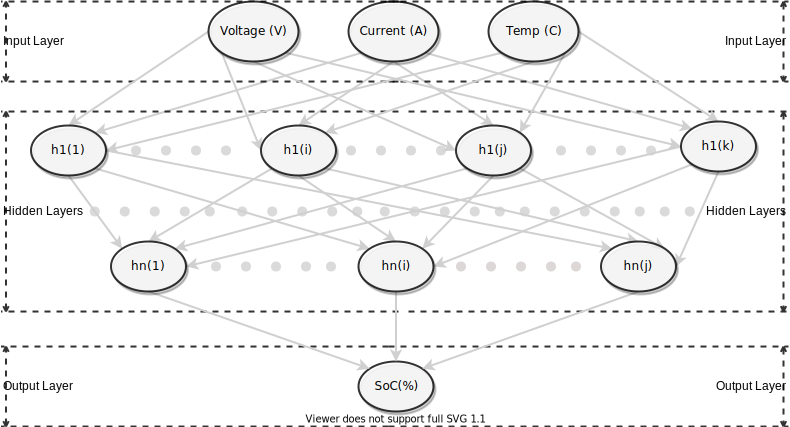
\includegraphics[width=13cm]{II_Body/images/SoC-RNN.png}
    \caption{Universal structure of RNN for SoC estimation.}
    \label{fig:RNN-structure}
\end{figure}
% In case the article did not specify the number of neurons per layer, the following equations have been used to get the initial raw estimation~\cite{eckhardt_choosing_2018}:
% \begin{equation}
%     \begin{split}
%         N_h &= \frac{N_s}{ a \left(N_i+N_o \right)} \ \ OR \ \ N_h = \frac{2}{3}\left(N_i+N_o \right) \\
%         N_i &\rightarrow \text{Number of input neurons} \\
%         N_o &\rightarrow \text{Number of output neurons} \\
%         N_s &\rightarrow \text{Number of samples in training data set} \\
%         \alpha &\rightarrow \text{An arbitrary scaling factor 2(5)-10}
%     \end{split}
% \end{equation}
%**Contrary to Hidden Layers as per their name, they obey only internally defined logic and connections.
%**That is why models are stable and reliable once created, cannot be changed, only retrainable with different data.
%A standard Hidden layer consisting of fully connected neurons called a Dense Layer.
%A standard Hidden layer, consisting of fully connected neurons and only one or no activation function, is called a Dense Layer.
%Within each cell of a Dense layer lies a single activation function.

%An Output Layer gets created from Dense Layer and commonly with no Activation function.
%: \textit{Simple, Exponential or Rectified Linear; Sigmoid and Hyperbolic Tangent functions}. \\
% \begin{itemize}
%     \item \textit{linear} - Simple Linear function
%     \item \textit{elu} - Exponential Linear function
%     \item \textit{relu} - Rectified Linear unit function
%     \item \textit{sigmoind} - Sigmoid function $sigmoid(x) = 1/1(1+exp(-x)$
%     \item \textit{tanh} - Hyperbolic Tangent function $$
% \end{itemize}

% Tanh and sigmoid definitions, equations and dropout.
%
Several activation functions for those layers are widely used in machine learning libraries for time-series problems~\cite{amidi_cs_2018}.
For the SoC prediction problem, all authors used the same function.
They experimentally confirmed that the best option for all hidden layers was the hyperbolic tangent function in \mbox{Equation~(\ref{eq:tanh})}.
The output layer used a sigmoid function as an activation to bound the result between zero and one, indicating the percentage of the charge, given by \mbox{Equation~(\ref{eq:sigmoid})}.
A dropout layer technique with a 20\% cutoff was applied to all hidden layers to prevent early data overfitting over long training periods.
\begin{equation}
    tanh(x) = \frac{sinh(x)}{cosh(x)}=\frac{e^x-e^{-x}}{e^x+e^{-x}}
    \label{eq:tanh}
\end{equation}
\begin{equation}
    \sigma(x) = \frac{1}{1+e^{-x}}
    \label{eq:sigmoid}
\end{equation}
%
%
%The common usage of the Dense layer in this paper is the Output Layer with no activation functions and a single neuron representing a single output SoC value.
%To apply multiple different without overcomplicating neurons, multiple layers with different or the same number of neurons or activations functions are applied.
%The more Hidden layers a network contains - the deeper and computationally complex a network becomes, also referred to as Deep Neural Networks. 
% Choosing the number of neurons for a first Hidden Layer does not have a golden rule.
% For this article, the following formula helps to make a good initial estimate based on the number of samples, Input and Output.\\
% \textbf{Equation}\\
% A common practice is to narrow each following Neurons by two from the previous one, to make a more accurate capture.
% To avoid overfitting data, except for data normalisation and Input sample shuffling in stateless models, a Dropout technique gets applied.
% Tensorflow has an internal implementation of Dropout for GRU and LSTM layers. A value of 0.2 (20\%) was applied to all RNN layers to minimise the overfitting possibility.

% Intro to vanishing gradient problem and gentle move to LSTM and GRU.
%
The efficiency of an RNN in a time-series problem is defined by the ability of the neurons to store memory as an internal state.
Over time, the memory of long-passed samples may fade away.
The problem is called the vanishing gradient, when the value needed to update the network weights shrinks as it propagates over time~\cite{rasifaghihi_predictive_2020}.
Long-term dependencies are not captured, since layers with a slight gradient do not significantly affect the system due to their insufficient weight change~\cite{rasifaghihi_predictive_2020,hochreiter_vanishing_1998}.
The more complicated structures of neurons tend to solve that problem.
% The gradient is the value used to update Neural Networks’ weight.
%"Therefore, layers that get a small gradient do not learn, and they cause the network to have short-term memory."
% https://www.bioinf.jku.at/publications/older/2304.pdf
%"With gradient-based learning methods, the current error signals have to 'flow back in time over the feedback connections to past inputs for building up adequate input storage. Long-term dependencies are hard to learn because of insufficient weight changes."

% Introduction statement to Gated Recurrent Unit and Long-Short Term Memory.
%
Two commonly used recurrent neural networks utilised memory cells, gated recurrent unit (GRU) and long short-term memory (LSTM), with possible extensions implemented by the referenced articles' authors.
% The GRU implementation will be used as a stateful technique by preserving a state from batch to batch with a single sample at a time.
The GRU and LSTM used a stateless approach, providing a fixed number of timestamps for all implemented models.
The stateless implementations with non-gradient-calculus-based optimisation algorithms were not used as part of this research because their effectiveness was not proven during preliminary work for this case.
%Implementation of the model based on simple RNN using multi-layer Dense(X) networks.~\cite{lees2010theoretical}
% a basic version of Recurrent Neural Network consists of fundamental layers with some neurons.
% \subsubsection{Implementation}
%     The input data for a network has been created using the Windowing technique, where \textbf{216k} sample of battery data, consisting of State Of Charge only, were separated on 500 sample windows.
%     As a result, the model outputs a single sample as SoC at the next Time Step. Using the Tensorflow library and calculating the number of Neurons using recommended formula \\
%     \textbf{THIS IS THE BEST PLACE FOR IT}. No other place suites as much.
%     The structure of the model ha\subsection{Training and Validation}

%s the following form. (Few Dense Layers+Dropount).
%     A Dropout layer has been used to prevent data overfitting. The selection of activation functions has been made through the data properties, which model has to fit in multiple trials.
% \subsubsection{Observation}
%     A simple Recurrent Neural Network has proven effective with simple Linear problems. However, with the battery state of charge, it cannot capture complicated features like the transition between Discharge and Charge or the process of Constant-Voltage Constant-Current charging. In applying battery utilisation inside Electrical Vehicle, this approach can be used only with some additional logic, such as Kalman Filters.
%     The best approach is to introduce more information about battery state and use a more complicated version of Time Series capable of memorising features with time, such as LSTM~\ref{sec: LSTM} and GRU~\ref{sec: GRU}.
    % The prediction results are discussed in Section~\ref{sec:results}.
%\subsection{Stateful Gradient Recurrent Unit (GRU) Algorithms and Implementations} \label{subsec:GRU}
%\subsection{LSTM with Attention}\label{sec:lstm-attention}
LSTM and GRU models made the most comonly used implemtation of Time -series predictions. TadeleMamo2020 research was intended to determine waknesses and improve the model introducing addition techniques into the default structure of training model***. \\
THe attention mechanissm used in ... \\
THe intention was to capture ... \\
\subsection{Implementation}
    Attention layer implementation was taken from \textbf{refernece} github repositry of ....
    
Implementation of the model based on TadeleMamo 2020 as the most recent and how to implement improvement to the model to make it better. Gracefully transition idea from here to my model, it is similar.

    %  Gated Recurrent Unit
% Definition of the GRU
%
\subsubsection{Gated Recurrent Unit (GRU) based models} \label{subsub:gru}
One of the methods proposed by Cho et al.~\cite{GRU_cho_properties_2014}, which improves the behaviour of the Neural network, is Gated Recurrent Unit.
Unlike a simple Recurrent NN with a single activation function in the cells, GRU implements different logics to deal with vanishing gradient, as per \mbox{Figure~\ref{fig:GRU-cell}}.
On top of the activation function, it adds two gates related to input and propagated sequences.
The reset gate $r_t$ controls the level information, which has to be ignored.
The update gate $i_t$ controls the impact of previous information on the current status.
The gates implemented by \textit{sigmoid} \mbox{Equation~\ref{eq:sigmoid}} and gated get updated with \mbox{Equations~\ref{eq:GRU-gates}}.
Both gates are related to cell input sequence $x_t$ and the memory cell's output at last time stamp $h_{t-1}$.
%The structure of the layers is similar to a Dense network, with similar input and output layers.
%\textbf{Y. Song~\cite{song_lithium-ion_2018} considered them less complex than another variation (LSTM-RNN) due to the usage of 2 gates rather than 3.}
% \footnote{Bigger value - bigger impact}..
%Weight W and bias b will be the training elements. Bias is added to each gate to increase network flexibility.\\
\begin{figure}[ht]%[htbp]
    \centering
    \includegraphics[width=\linewidth]{II_Body/GRU/images/GRU.jpg}
    \caption{Gated Recurrent Unit Cell}
    \label{fig:GRU-cell}
\end{figure}
\begin{equation}
    \begin{split}
        f_t &= \sigma \left (W_{f} \left [h_{t-1}, x_t \right ] + b_f \right ) \\
        i_t &= \sigma \left (W_{i} \left [h_{t-1}, x_t \right ] + b_i \right )
    \end{split}
    \label{eq:GRU-gates}
\end{equation}
%The standard activation function or content of the memory gets modified with equation~\ref{eq:GRU-output}, where \textit{func} represent the activation function and $\ast$ multiplication by element.
The memory cell output $h_t$ get calculated through the early chosen activation function, $tanh$ in \mbox{Equation~\ref{eq:GRU-output}}.
The $\ast$ stand for multiplication by element.
\begin{equation}
    \begin{split}
        \hat{h_t} &= tanh \left (W_{\hat{h}} \left [f_t \ast h_{t-1}, x_t \right ] + b_{\hat{h}} \right ) \\
        h_t &= \left (1-i_t \right ) h_{t-1}+i_t \hat{h_t}
    \end{split}
    \label{eq:GRU-output}
\end{equation}
% The GRU can act both as a stateful and stateless cell for the model by implementing the model training library.
% For comparison, a Stateful cell will be used per implementation from Song et al.~\cite{song_lithium-ion_2018} and similar articles.
%
% By implementing a model training library, the GRU can act as a stateful and stateless cell for the model.
%(1) - not even count. The method proposed by Y.Song2018, Remaining Useful Life (RUL), \textcolor{red}{uses Capacity only. Nothing more. However, no one mentioned the Statefulnes of GRU models. This would be the best place to introduce it once properly figured out.} \\[2pc]
%
%
% (3) Method proposed by B.Xiao2019 enhances GRU model training with an Ensemble optimisation method.
% Instead of utilising standard Adam optimiser, it combines Nadam and Adamax by running one after another.
% For the first 1/3 training iterations (epochs), Nadam optimiser was used for model pre-training due to its' fast converging speed, then Adamax for model fine-tuning to determine the remaining parameters. \\
% The algorithms for model fitting are as follow \\
%
%
% (8) Similar to LSTM, a Gated Recurrent Unit is intended to solve the vanishing gradient problem.
%     Unlike Chemali2017 implementation, where the training set has consisted of input data sequences with stateles model, BinXio2019 used a stateful model within batches. In addition, it introduced a technique of optimisation to the speedup training process.
%     Implementation of the model based on BinXio or someone else. Introduce their implementation and how to improve optimisation using two algorithms per their discussion.

% \subsection{Implementation}
%     Instead of implementing learning based on Battery Capacity, the following method will use the State of Charge as an input and output, similar to the Dense example. Folowing table highglights parameters, which proven to be most effective during the tests.  \textbf{Table of the parameters like BinXiao}. The activation function was selected as the \textit{tanh} \textbf{the number of sample experementaly was selected as 500?? .} \\
%     \textbf{I have found the place to describe statefulnes for the first time. Potentially, it needs to implement properly. Use the following link to understand how to keep it between batches.}
%https://machinelearningmastery.com/time-series-prediction-lstm-recurrent-neural-networks-python-keras/


    \subsubsection{Long-Short Term Memory based models} \label{subsub:lstm}
The second method and the most commonly used in the Time-series Machine learning model is the Long Short-Term Memory Cell~\cite{LSTM_Hochreiter1997}.
Similar to GRU, LSTM models tend to preserve long-term dependencies in the extended data sequences.
For a longer existence, it became the most widely used type of RNN, used in those types of applications.
Figure~\ref{fig:LSTM-cell} summarises the internal cell logic.
%Currently, the most common usage of the Time-series Machine LEarning model is the prediction of stock prices, weather prognosition or any other time dependant data.
%However, the most common problem for any of those scenarios is vanishing gradient.
%Long range data tend to fade away from the model, which impacts overall prediction.
\begin{figure}[ht]%[htbp]
    \centering
    \includegraphics[width=0.7\linewidth]{II_Body/LSTM/images/LSTM.jpg}
    \caption{Long Short-Term Memory Cell}
    \label{fig:LSTM-cell}
\end{figure}
Unlike GRU, this cell utilises three gates instead of 2.
The update gate gets replaced with separate input $i_t$ and output $o_t$, as per equation~\ref{eq:LSTM-gates}.
All gets utilise the same sigmoid equation~\ref{eq:sigmoid}.
%\textcolor{red}{Those are clasical LSTM approaches. Using history sizes, no Stateless methods.}
%Unlike with GRU, the update gates renamed as an input gate $i_t$, with the same equation. Even that the forget gate $f_t$ is the same, model utilises another one, output gate $g_t$ as per Equations~\ref{eq:LSTM-gates}.
\begin{equation}
    \begin{split}
        f_t &= \sigma \left(W_f \left[h_{t-1}, x_t \right] + b_f \right) \\
        i_t &= \sigma \left(W_i \left[h_{t-1}, x_t \right] + b_i \right) \\
        o_t &= \sigma \left(W_o \left[h_{t-1}, x_t \right] + b_o \right) \\    
    \end{split}
    \label{eq:LSTM-gates}
\end{equation}
The main difference between LSTM and GRU lies in the cell state calculation.
Using the same $tanh$ activation function, Equation~\ref{eq:LSTM-output} describes how cells will be updated and propagated further.
The $c_t$ represents the cell state at a timestamp.
\begin{equation}
    \begin{split}
        \hat{c_t} &= tanh \left(W_c \left[h_{t-1}, x_t \right] + b_c \right) \\
              c_t &= f_t c_{t-1}+i_t \hat{c_t} \\
              h_t &= o_t*tanh \left(c_t \right)II_Body
    \end{split}
    \label{eq:LSTM-output}
\end{equation}
% $c_t \rightarrow$ cell state (memory) at timestep $t$ \\
% $\hat{c_t} \rightarrow$ candidate for cell state \\
% $* \rightarrow$ element wise multiplication \\
Like the GRU cell type, the model training Library supports both stateful and stateless utilisation of the LSTM model.
It will be used as a Stateless cell for further comparison based on Chemali et al.~\cite{Chemali2017} and similar articles.
%
%
% (7) \textcolor{red}{The most complicated one}. Method by WeiZhang2020. Adaptive Time-series prediction on online validation. Data taken directly during cycling batteries.
% \textbf{I have to study this properly first. Long-Horizon, as they called it, more useful ti State if Health. This should be the end of them.}
\subsubsection{Attention Layer}
The research conducted by~\cite{mamo_long_2020} was intended to determine weaknesses and improve the model introducing addition techniques into the default structure of the training model.
They added Attention Layer~\cite{yang_hierarchical_2016} between LSTM and fully connected layers to improve accuracy and replace traditional gradient optimiser with probability-based Differential Evolution.
Figure~\ref{fig:attention} summarises the model structure, and equations~\ref{eq:AttentionWithContext} and~\ref{eq:Addition} define the internal logic between hidden layers and output.

%
%
%bla bla bla... I am exosted, I hgete this part I have no idea what to write and have no desire to research more.
The implementation of the Attention layer does not get provided with the Machine Learning library.
The source code from Winata research~\cite{winata_attention-based_2018} has been used instead.
The open-source code publicly accesses through Github source~\cite{attention_8461990}.
Details in terms of optimiser usage and replacement are justified in subsection~\ref{subsec:optimisers}.
In the State of Charge estimation, the attention layer addresses two shortcomings of LSTM: replacing the traditional method of recursively constructing LSTM depth and located after the output of the primary layer, just before the model Dense layer output~\cite{mamo_long_2020}.
\begin{figure}[htbp]
    \centering
    \includegraphics[width=0.35\linewidth]{II_Body/LSTM/images/AttenrionDrawing.png}
    \caption{Attention based architecture}
    \label{fig:attention}
\end{figure}
\begin{equation}
    \begin{split}
        \hat{u_t} &= tanh \left(W h_{t} + b \right) \\
             \alpha_t &= \frac{exp(u^T u)}{\sum_t(exp(u_t^T u))} \\
              v_t &= \alpha_t*h_t, v in time t
    \end{split}
    \label{eq:AttentionWithContext}
\end{equation}
\begin{equation}
    \begin{split}
        v = \sum_t(\alpha_t * h_t)
    \end{split}
    \label{eq:Addition}
\end{equation}

% \subsection{Implementation}
%     Following table higlighs parameters, which provided best results for their experements.
%     \textbf{Table of the parameters.}
%     The network will be the one discussed above.
%     Model itself will be multi-feature based with follwoing parameters: Voltage \textit{V(t)}, Current \textit{A(t)} and Temperature \textit{C(t)}, where \textit{t} represents a time-stamp. Each feature will contain equal amount of sample and each will be feed in input column vector. As a result, a single input will have following form: \\
%     % [V(0)], [I(0)], [T(0)] \\
%     % [V(1)], [I(1)], [T(1)] \\
%     % [V(n)], [I(n)], [T(n)] \\
%     where \textit{n} is the history size.
%     The output vector will be a State of Charge \textit{SoC(\%)} percentage up to 2 decimal places, within range 0 to 1 and time stamp \textit{n}: \\
%     % [SoC(n)] \\
%     As a result the shape of input and output data will be: X(0)=(n,3) and Y(0)=(1)
%     The entire dataset will use single-step windowing tecnhinue with no bathces to save memory and utilsase \textbf{stateless}* \footnote{Need to discuss this with Holmes.} model. \\
%     The Generated dataset of sample size \textit{k}, will consist of two Tensor input/output Vectors of following shape: \\
%     X = (k-n,n,3), Y = (k-n,1).
%     The variable type for computation was selected to be float32.
%     To keep Denerated dataset simple, no batching approach spared from dealing with 4-dimensional input vectors.
% \subsection{Prediction results}


%     Implementation of the model based on Chemali2017. Application for our section and results. Refer to methodology from time to time.
    \subsection{Optimisers} \label{subsec:optimisers}
    \subsection{Types of optimisers}
The selection of the optimiser defines how fast the model will achieve the local minimum.
Different algorithms utilised several improvements to achieve an optimum result more quickly and avoid overfitting.
All model share the same parameter, the learning rate $\alpha$, which acts as a step to update predictions.
%  Classic Stochastic Gradient Descent
% Explanation
%
\subsubsection{Classic and Momentum Stochastic Gradient Descent Algorithms}
One of the simplest methods to optimise the model is the stochastic gradient descent (SGD), Algorithm~\ref{alg:SGDwM}.
% \begin{algorithm}\captionsetup{labelfont={sc,bf}, labelsep=newline}
%   \caption{Stochastic Gradient Descent (SGD) optimisation}
%   \begin{algorithmic}[1]
%     \STATE \textbf{Number of input samples} \\ $N\gets length(\textit{input data})$\\
%     \STATE \textbf{Size of windows} \\ $S\gets length(V_{i..n})$\\
%     \STATE Input: $x_n = [V_{i..n}, I_{i..n}, T_{i..n}] - $Shape: $X = (N, S, 3)$
%     \STATE Output:$y_n = [SoC_{n}] - $Shape:$Y = (N, 1)$
%     \STATE Define Loss function: $L$ \\
%            Get hyperparameters: $\alpha$
%     \WHILE{$W_t \text{ not converge}$}
%     \STATE $t \gets t+1$
%     \STATE $g_t \gets \nabla_\phi L_t (W_{t-1})$ \COMMENT{Obtain gradient}
%     \STATE $W_t \gets W_{t-1} - \alpha g_t $ \COMMENT{Update parameters}
%     \ENDWHILE
%   \end{algorithmic}
%   \label{alg:SGD}
% \end{algorithm}
The SGD optimiser utilises a simple gradient update with the following learning rate: \mbox{Algorithm~\ref{alg:SGDwM}, Line~\ref{alg:SGDwM-Line-Gradient}}.
% uses fewer calculations and achieves results slower* Higher chances of not achieving the minimum
% Unlike improved versions, this algorithm has the potential of missing optimum value.
The extension of SGD, which Jiao et al.~\cite{jiao_gru-rnn_2020} used, applies a single momentum calculation, \mbox{Algorithm~\ref{alg:SGDwM}, to the classical SGD Line~\ref{alg:SGDwM-Line-Moment}}.
In the text, this is referred to as the stochastic gradient descent with momentum (SGDw/M).
It increases the algorithm's performance by improving the convergence speed compared to the classical~version.
\begin{algorithm}[H]%\captionsetup{labelfont={sc,bf}, labelsep=newline}
  \caption{Stochastic gradient descent with momentum optimisation.}
  \begin{algorithmic}[1]
    \STATE \textbf{Number of input samples} \\ $N\gets length(\textit{input data})$\\
    \STATE \textbf{Size of windows} \\ $S\gets length(V_{i..n})$\\
    \STATE Input: $x_n = [V_{i..n}, I_{i..n}, T_{i..n}] - $Shape: $X = (N, S, 3)$
    \STATE Output:$y_n = [SoC_{n}] - $Shape:$Y = (N, 1)$
    \STATE Define loss function: $L$ \\
    Get hyperparameters: $\alpha, \beta_1$
    \WHILE{$W_t \text{ does not converge}$}
      \STATE $t \gets t+1$
      \STATE $g_t \gets \nabla_W L_t (W_{t-1})$ \COMMENT{obtain gradient \label{alg:SGDwM-Line-Gradient}}
      \STATE $m_t \gets \beta_1 m_{t-1}+(1-\beta_1) g_t $ \COMMENT{1st moment calculation\label{alg:SGDwM-Line-Moment}}
      \STATE $W_t \gets W_{t-1} - \alpha m_t $ \COMMENT{update parameters}
    \ENDWHILE
  \end{algorithmic}
  \label{alg:SGDwM}
\end{algorithm}

% Noising the data
%
% To improve accuracy, Jiao introduced noise to the data to be able to capture more variant information.
% Due to the amount of data provided and comparison with other methods, noise variance will not be used in this implementation.
% \mbox{Table~\ref{tab:params-jiao}} provides parameters selection for the optimiser.
% \begin{table}[ht]
%     \renewcommand{\arraystretch}{1.3}
%     \caption{Hyper-Parameters as per Jiao \textit{et al.}~\cite{jiao_gru-rnn_2020}}
%     \centering
%     \label{tab:params-jiao}
%     \resizebox{\columnwidth}{!}{
%     \begin{tabular}{ l c c }
%       \hline\hline \\[-3mm]
%         Method     & $\alpha$ & $\beta_1 $  \\
%         \hline
%         SGDw/M
%                 & $0.001$ & $0.8$  \\% 0.0000001
%         \hline\hline
%     \end{tabular}
%     }
% \end{table}
% \newpage
\subsubsection{Adam and Robust Online Adam}
The most commonly and by default used in Time-series prediction is Adaptive Moment Estimation~\cite{kingma_adam_2017} (Adam) optimiser.
The algorithm below highlights the steps required to update model weights and bias as per the source.
On top of two constants $\beta$ used for momentum calculation, the algorithm uses $\epsilon$, which referred to as fuzz factor.

%
%
Javid et al.~\cite{javid_adaptive_2020} extended the default $Adam$ algorithm introducing a Robust Online version of Adam, Line 10-12.
Adding the direct influence of loss function to the gradient update adds an online calculation to regular $Adam$ correction.
Table~\ref{tab:adam-params} highlight method-specific parameter selection for the optimiser.
The framework library contained no inbuild implementation of the Robust optimiser.
Instead, it was implemented from the first principal and overwriting the model training procedure.
The code itself can be located in Appendix~\ref{}
\begin{algorithm}\captionsetup{labelfont={sc,bf}, labelsep=newline}
  \caption{Adaptive Moment Estimation (Adam) optimisation}
  \begin{algorithmic}[1]
    \STATE \textbf{Number of input samples} \\ $N\gets length(\textit{input data})$\\
    \STATE \textbf{Size of windows} \\ $S\gets length(V_{i..n})$\\
    \STATE Input: $x_n = [V_{i..n}, I_{i..n}, T_{i..n}] - $Shape: $X = (N, S, 3)$
    \STATE Output:$y_n = [SoC_{n}] - $Shape:$Y = (N, 1)$
    \STATE Define Loss function: $L$ \\
           Get hyperparameters: $\alpha, \beta_1, \beta_2, \epsilon$
    \WHILE{$W_t \text{ not converge}$}
    \STATE $t \gets t+1$
    \STATE $g_t \gets \nabla_W L_t (W_{t-1})$ \COMMENT{Obtain gradient}
    \STATE $m_t \gets \beta_1 m_{t-1}+(1-\beta_1) g_t $ \COMMENT{$1_{st}$ moment calculation}
    \STATE $\upsilon_t \gets \beta_2 \upsilon_{t-1}+ \left(1-\beta_2 \right)g^2_t $ \COMMENT{$2_{nd}$ moment calculation \label{alg:Adam-Line-2Moment}}
    \STATE $\hat{m_t} \gets \frac{m_t}{1-\beta^t_1}$ \COMMENT{Corrected $\hat{m_t}$}
    \STATE $\hat{\upsilon_t} \gets \frac{\upsilon_t}{1-\beta^t_2} $ \COMMENT{Corrected $\hat{\upsilon_t}$}
    \STATE $W_t \gets W_{t-1}- \alpha \frac{\hat{m_t}}{\sqrt{\hat{\upsilon_t}}+\epsilon} $ \COMMENT{Update parameters}
    \ENDWHILE
  \end{algorithmic}
  \label{alg:Adam}
\end{algorithm}
% \begin{tabular}{ l } 
%     \hline
%     Algorithm Adam optimisation  \\
%     \hline
%     %\ \ \textbf{Input:} Data sample with shape=\left(1,500,1,3\right)\\ 
%     %\ \ \textbf{Output:} Predicted SoC shape=\left(1,500,1\right)\\ 
%     \ \ \ 1: Define I/O and Params: $\alpha, \beta_1, \beta_2, \epsilon $ \\
%     \ \ \ 2: Define loss function $L$ \\
%     \ \ \ 3: \textbf{while} $\phi_t$ not converge \textbf{do}: \\
%     \ \ \ 4: \ \ $t \leftarrow t + 1$ \\
%     \ \ \ 5: \ \ $g_t \leftarrow \nabla_\phi L_t \left(\phi_{t-1} \right) $ \text{\ \ \ //Obtain Gradient}\\
%     \ \ \ 6: \ \ $m_t \leftarrow \beta_1 m_{t-1}+ \left(1-\beta_1 \right)g_t $ \text{//$1^{st}$moment }\\
%     \ \ \ 7: \ \ $\upsilon_t\ \leftarrow \beta_2 \upsilon_{t-1}+ \left(1-\beta_2 \right)g^2_t $ \text{//$2^{nd}$moment }\\
%     \ \ \ 8: \ \ $\hat{m_t}\ \ \leftarrow \frac{m_t}{1-\beta^t_1}$ \text{Correct \ \ }$\hat{m_t}$\\
%     \ \ \ 9: \ \ $\hat{\upsilon_t}\ \ \leftarrow \frac{\upsilon_t}{1-\beta^t_2} $ \text{Correct \ \ }$\hat{\upsilon_t}$ \\ \\ \\ \\
%     \ \  10: \ \ $\phi_t \leftarrow \phi_{t-1}- \alpha \frac{\hat{m_t}}{\sqrt{\hat{\upsilon_t}}+\epsilon} $ \\
%     \ \  11: \textbf{end while} \\
%     \hline
% \end{tabular}
\begin{algorithm}\captionsetup{labelfont={sc,bf}, labelsep=newline}
  \caption{Robust Online Adaptive Moment Estimation (Adam) optimisation}
  \begin{algorithmic}[1]
    \STATE \textbf{Number of input samples} \\ $N\gets length(\textit{input data})$\\
    \STATE \textbf{Size of windows} \\ $S\gets length(V_{i..n})$\\
    \STATE Input: $x_n = [V_{i..n}, I_{i..n}, T_{i..n}] - $Shape: $X = (N, S, 3)$
    \STATE Output:$y_n = [SoC_{n}] - $Shape:$Y = (N, 1)$
    \STATE Define Loss function: $L$ \\
           Get hyperparameters: $\alpha, \beta_1, \beta_2, \beta_3, \epsilon$
    \WHILE{$W_t \text{ not converge}$}
    \STATE $t \gets t+1$
    \STATE $g_t \gets \nabla_\phi L_t (W_{t-1})$ \COMMENT{Obtain gradient}
    \STATE $m_t \gets \beta_1 m_{t-1}+(1-\beta_1) g_t $ \COMMENT{$1_{st}$ moment calculation}
    \STATE $\upsilon_t \gets \beta_2 \upsilon_{t-1}+ \left(1-\beta_2 \right)g^2_t $ \COMMENT{$2_{nd}$ moment calculation}
    \STATE $\hat{m_t} \gets \frac{m_t}{1-\beta^t_1}$ \COMMENT{Corrected $\hat{m_t}$}
    \STATE $\hat{\upsilon_t} \gets \frac{\upsilon_t}{1-\beta^t_2} $ \COMMENT{Corrected $\hat{\upsilon_t}$}
    \STATE $r_t \gets \parallel L_t\left(W_{t-1}\right)/L_t\left(W_{t-2}\right) \parallel $ \COMMENT{Relative prediction error term of the loss function}
    \STATE $d_t \gets \beta_3 d_{t-1}+\left(1-\beta_3\right)r_t $ \COMMENT{$3^{rd}$ moment calculation}
    \STATE $W_t \gets W_{t-1}- \alpha \frac{\hat{m_t}}{d_t\sqrt{\hat{\upsilon_t}}+\epsilon} $ \COMMENT{Update parameters}
    \ENDWHILE
  \end{algorithmic}
  \label{alg:RoAdam}
\end{algorithm}
% \begin{tabular}{ l } 
%     \hline
%     Algorithm Robust Adam optimisation  \\
%     \hline
%     %\ \ \textbf{Input:} Data sample with shape=\left(1,500,1,3\right)\\ 
%     %\ \ \textbf{Output:} Predicted SoC shape=\left(1,500,1\right)\\ 
%     \ \ \ 1: Define I/O and Params: $\alpha, \beta_1, \beta_2, \beta_3, \epsilon $ \\
%     \ \ \ 2: Define loss function $L$ \\
%     \ \ \ 3: \textbf{while} $\phi_t$ not converge \textbf{do}: \\
%     \ \ \ 4: \ \ $t \leftarrow t + 1$ \\
%     \ \ \ 5: \ \ $g_t \leftarrow \nabla_\phi L_t\left(\phi_{t-1}\right) $ \\
%     \ \ \ 6: \ \ $m_t \leftarrow \beta_1 m_{t-1}+\left(1-\beta_1\right)g_t $ \\
%     \ \ \ 7: \ \ $\upsilon_t\ \leftarrow \beta_2 \upsilon_{t-1}+\left(1-\beta_2\right)g^2_t $ \\
%     \ \ \ 8: \ \ $\hat{m_t}\ \ \leftarrow \frac{m_t}{1-\beta^t_1}$ \\
%     \ \ \ 9: \ \ $\hat{\upsilon_t}\ \ \leftarrow \frac{\upsilon_t}{1-\beta^t_2} $ \\
%     \ \ \ // Relative prediction error term of the loss function: \\
%     \ \ 10: \ \ $r_t \leftarrow \parallel L_t\left(\phi_{t-1}\right)/L_t\left(\phi_{t-2}\right) \parallel $ \\
%     \ \ 11: \ \ $d_t\ \leftarrow \beta_3 d_{t-1}+\left(1-\beta_3\right)r_t $ \text{//$3^{rd}$moment }\\
%     \ \ 12: \ \ $\phi_t \leftarrow \phi_{t-1}- \alpha \frac{\hat{m_t}}{d_t\sqrt{\hat{\upsilon_t}}+\epsilon} $ \\
%     \ \ 13: \textbf{end while} \\
%     \hline
% \end{tabular}
\begin{table}[htbp]
    \centering
    \caption{Adam, specific parameters}
    \label{tab:adam-params}
    \begin{tabular}{ p{6.0cm} p{1.5cm} p{1.5cm} p{1.5cm} p{1.5cm} p{1.5cm}  }
        \hline
        Source     & $\alpha$ & $\beta_1 $ & $\beta_2$ & $\beta_3$ &  $\epsilon$ \\
        \hline
        Song et al.~\cite{song_lithium-ion_2018} \& Chemale et al.~\cite{Chemali2017}
                & $0.001$ & $0.9$ & $0.999$ & |   &$10^{-8}$ \\% 0.0000001
        Javid et al.~\cite{javid_adaptive_2020}
                & $0.001$ & $0.9$ & $0.999$ & $0.999$ &$10^{-8}$ \\% 0.0000001
        %\hline
        \hline
    \end{tabular}
\end{table}



%  Ensemble optimisation
% Explanation
%
\subsubsection{Ensemble optimisation with Nesterov Momentum Adam and AdaMax}
The Adam algorithm remains the most commonly used optimiser.
The reason behind changing it to another lie in two potential issues.
The first is if the training converges, which may not happen at all~\cite{reddi_convergence_2019}.
The second is if the optimal solution gets frequently missed at large learning steps~\cite{wilson_marginal_2017}.
Xiao \textit{et al.}~\cite{xiao_accurate_2019} proposed a novel alternative of combining several optimisers to address those issues.
The new ensemble optimisation algorithm is based on the combination of Nesterov Momentum Adam (Nadam), \mbox{Algorithm~\ref{alg:nadam}}~\cite{dozat_nadam_2016}, and the AdaMax, \mbox{Algorithm~\ref{alg:adamax}}~\cite{kingma_adam_2017}, at certain moments of training.

% Nadam's advantage over Adam
%
The Nadam optimiser \mbox{Algorithm~\ref{alg:nadam}} extends the Adam, which implements the Nesterov momentum~\cite{dozat_nadam_2016}.
\mbox{Ag~\ref{alg:nadam}, Ln~\ref{alg:Nadam-Line} and Ln~\ref{alg:Nadam-Line-update}} add additional calculations involving gradient and parameters update, intended to improve convergence speed.
% \textcolor{red}{Another error. This time with SQRT. According to Adam and the source code in TF for Nadam, epsilon is not inside sqrt(). Although the original article stands otherwise, Xiao also corrected it. I am sticking with whatever I have at TF. There is no $\beta_i$ and no $\beta_2$ in the second moment update equation. All of that was corrected.}
\begin{algorithm}\captionsetup{labelfont={sc,bf}, labelsep=newline}
    \caption{Nesterov Adaptive Moment Estimation (Nadam) optimisation}
    \begin{algorithmic}[1]
      \STATE \textbf{Number of input samples} \\ $N\gets length(\textit{input data})$\\
      \STATE \textbf{Size of windows} \\ $S\gets length(V_{i..n})$\\
      \STATE Input: $x_n = [V_{i..n}, I_{i..n}, T_{i..n}] - $Shape: $X = (N, S, 3)$
      \STATE Output:$y_n = [SoC_{n}] - $Shape:$Y = (N, 1)$
      \STATE Define Loss function: $L$ \\
             Get hyperparameters: $\alpha, \beta_1, \beta_2, \epsilon$
      \WHILE{$W_t \text{ not converge}$}
      \STATE $t \gets t+1$
      \STATE $g_t \gets \nabla_\phi L_t (W_{t-1})$ \COMMENT{Obtain gradient}
      \STATE $m_t \gets \beta_1 m_{t-1}+(1-\beta_1) g_t $ \COMMENT{$1_{st}$ moment calculation}
      \STATE $\upsilon_t \gets \beta_2 \upsilon_{t-1}+ \left(1-\beta_2 \right)g^2_t $ \COMMENT{$2_{nd}$ moment calculation}
      \STATE $\hat{m_t} \gets \frac{m_t}{1-\beta^t_1}$ \COMMENT{Corrected $\hat{m_t}$}
      \STATE $\hat{\upsilon_t} \gets \frac{\upsilon_t}{1-\beta^t_2} $ \COMMENT{Corrected $\hat{\upsilon_t}$}
      \STATE $\hat{g_t} \gets \frac{g_t}{1-\prod\nolimits_{i = 1}^{k}\beta^t_2} $ \COMMENT{Corrected $\hat{g_t}$\label{alg:Nadam-Line}}
      \STATE $W_t \gets W_{t-1}-\alpha
                          \frac{\left(\beta^{k+1}_1\hat{m_t}+\left(1-\beta^t_1\right)\hat{g_t}\right)}
                               {\sqrt{\hat{\upsilon_t}}+\epsilon}$
                               \COMMENT{Update parameters\label{alg:Nadam-Line-update}}
      % \STATE $W_t \gets W_{t-1}- \alpha \frac{\hat{m_t}}{\sqrt{\hat{\upsilon_t}}+\epsilon} $ // ??
      \ENDWHILE
    \end{algorithmic}
    \label{alg:nadam}
\end{algorithm}

% AdaMax advantages over Adam
%
\mbox{Algorithm~\ref{alg:adamax}} in the ensemble sequence is AdaMax~\cite{kingma_adam_2017}, another modification of the Adam.
The second-order moment on \mbox{Ag~\ref{alg:adamax}, Ln~\ref{alg:AdaMax-Line}} gets replaced with the infinity norm of the moment.
As a result, Xiao \textit{et al.}~\cite{xiao_accurate_2019} considered AdaMax to have a stable weight updating rule and be used in the fine-tuning phase since its' advantage lies in the reduction of gradient fluctuation. 
\begin{algorithm}\captionsetup{labelfont={sc,bf}, labelsep=newline}
    \caption{Adaptive Moment Estimation based on the infinity norm (Adamax)}
    \begin{algorithmic}[1]
      \STATE \textbf{Number of input samples} \\ $N\gets length(\textit{input data})$\\
      \STATE \textbf{Size of windows} \\ $S\gets length(V_{i..n})$\\
      \STATE Input: $x_n = [V_{i..n}, I_{i..n}, T_{i..n}] - $Shape: $X = (N, S, 3)$
      \STATE Output:$y_n = [SoC_{n}] - $Shape:$Y = (N, 1)$
      \STATE Define Loss function: $L$ \\
             Get hyperparameters: $\alpha, \beta_1, \beta_2, \epsilon$
      \WHILE{$W_t \text{ not converge}$}
      \STATE $t \gets t+1$
      \STATE $g_t \gets \nabla_\phi L_t (W_{t-1})$ \COMMENT{Obtain gradient}
      \STATE $m_t \gets \beta_1 m_{t-1}+(1-\beta_1) g_t $ \COMMENT{$1^{st}$ moment calculation}
      \STATE $\upsilon_t \gets max\left(\beta_2\upsilon_{t-1}, |g_t|\right) $ \COMMENT{Corrected $\hat{\upsilon_t}$ \label{alg:AdaMax-Line}}
      % \STATE $W_t \gets W_{t-1}- \alpha \frac{1}{1-\beta^t_1}\frac{m_t}{\upsilon_t} $
      \STATE $W_t \gets W_{t-1}- \alpha \frac{m_t}{(1-\beta^t_1)(\upsilon_t+\epsilon)} $ \COMMENT{Update parameters}
      \ENDWHILE
    \end{algorithmic}
    \label{alg:adamax}
\end{algorithm}

%
%
Xiao \textit{et al.}~\cite{xiao_accurate_2019} considered separating the training process into two stages: pre-training and fine-tuning.
Based on their observations: \textit{``The purpose of the pre-training phase is to endow the GRU model with the appropriate parameters to capture inherent features of the training samples.
The Nadam algorithm uses adaptive learning rates and approximates the gradient using the Nesterov momentum, thereby ensuring fast convergence of the pre-training process."}~\cite[p.~54195]{xiao_accurate_2019}.
The selection of the second algorithm is trivial.
Xiao \textit{et al's}.~\cite{xiao_accurate_2019} selection of AdaMax is defined by fast-convergence to a more stable value for further parameter adjustment.
% \textcolor{red}{I'll be cursed. No, epsilon does. In the TensorFlow implementation, epsilons are added to the vt. Corrected formula added, but commented out. \\
%Remarks made by Xiao justify the usage of the Ensemble algorithm. How would I reprase it into something shorter}\\
%\textit{Remark 1:} The purpose of the pre-training phase os to endow the GRU model with the appropriate parameters to capture the inherent features of the training samples. The Nadam algorithm uses adaptive learning rates and approximates the gradient through the Nesterov momentum, ensuring fast convergence of the pre0training process.
%\textit{Remark 2:} The purpose of the fine-tuning phase is to adjust the parameters further to achieve greater accuracy using the AdaMax algorithm, which converges to a more stable value. \\ \\
The proposed Ensamble algorithm combines both methods for single GRU training, \mbox{Algorithm~\ref{alg:ENS}}.
It describes the adapted version of the Ensemble algorithm, used by the model training procedures, with Nadam for pre-training and AdaMax for fine-tuning phases.
From the results of Xiao \textit{et al.}'s~\cite{xiao_accurate_2019} work $<p_{1}$ and $<p_{2}$ had the same 100 number of epochs.
This scenario will use the value of $<p_{2}$ at the moment the model reaches an overfit with the first phase.
The value of the learning rate will be set to the minimum possible, defined by the research.
\begin{algorithm}\captionsetup{labelfont={sc,bf}, labelsep=newline}
    \caption{Ensemble optimisation training process}
        \begin{algorithmic}[1]
            % \STATE \textbf{Input:} Data sample with shape=(1,500,1,3) 
            % \STATE \textbf{Output:} Predicted SoC shape=(1,1,1)
            \STATE Setup model. Split total number of epoch by 30\% to $p_{1}$ and $p_{2}$ or until model overfits at $p_{2}$
            \STATE Initialise parameters
            \WHILE{epoch  $<p_{1}$:}
                \IF{epoch $<p_{2}$:}
                    \STATE \COMMENT{pass if already compiled with Nadam}
                    \STATE compile model with Nadam parameters. \COMMENT{pre-training phase}
                \ELSE
                    \STATE \COMMENT{pass if already compiled with AdaMax}
                    \STATE compile model with AdaMax parameters. \COMMENT{fine-tuning phase}
                \ENDIF
                \STATE train for a single epoch
            \ENDWHILE
        \end{algorithmic}
    \label{alg:ENS}
\end{algorithm}
%\textcolor{red}{Descibe what shape has been used. Single sample, history length, batch size (if applicable), features number}

%
%
% \mbox{Table~\ref{tab:ensemble-params}} higlights hyper parameters selected by Xiao et al.~\cite{xiao_accurate_2019}.
% \begin{table}[htbp]
%     \renewcommand{\arraystretch}{1.3}
%     \caption{Ensemble, specific parameters}
%     \centering
%     \label{tab:ensemble-params}
%     \resizebox{\columnwidth}{!}{
%     \begin{tabular}{ l c c c c }
%         \hline\hline \\[-3mm]
%         Optimiser     & $\alpha$ & $\beta_1 $ & $\beta_2$ &   $\epsilon$ \\
%         \hline
%         Nadam
%                 & $0.001$ & $0.99$ & $0.999$ & $10^{-8}$ \\% 0.0000001
%         AdaMax
%                 & $5*10^{-4}$ & $0.99$ & $0.999$ & $10^{-8}$ \\% $10^{-8}$
%         \hline
%     \end{tabular}
%     }
% \end{table}


        %  Classic Stochastic Gradient Descent
% Explanation
%
\subsubsection{Classic and Momentum Stochastic Gradient Descent Algorithms}
One of the simplest methods to optimise the model is the stochastic gradient descent (SGD), Algorithm~\ref{alg:SGDwM}.
% \begin{algorithm}\captionsetup{labelfont={sc,bf}, labelsep=newline}
%   \caption{Stochastic Gradient Descent (SGD) optimisation}
%   \begin{algorithmic}[1]
%     \STATE \textbf{Number of input samples} \\ $N\gets length(\textit{input data})$\\
%     \STATE \textbf{Size of windows} \\ $S\gets length(V_{i..n})$\\
%     \STATE Input: $x_n = [V_{i..n}, I_{i..n}, T_{i..n}] - $Shape: $X = (N, S, 3)$
%     \STATE Output:$y_n = [SoC_{n}] - $Shape:$Y = (N, 1)$
%     \STATE Define Loss function: $L$ \\
%            Get hyperparameters: $\alpha$
%     \WHILE{$W_t \text{ not converge}$}
%     \STATE $t \gets t+1$
%     \STATE $g_t \gets \nabla_\phi L_t (W_{t-1})$ \COMMENT{Obtain gradient}
%     \STATE $W_t \gets W_{t-1} - \alpha g_t $ \COMMENT{Update parameters}
%     \ENDWHILE
%   \end{algorithmic}
%   \label{alg:SGD}
% \end{algorithm}
The SGD optimiser utilises a simple gradient update with the following learning rate: \mbox{Algorithm~\ref{alg:SGDwM}, Line~\ref{alg:SGDwM-Line-Gradient}}.
% uses fewer calculations and achieves results slower* Higher chances of not achieving the minimum
% Unlike improved versions, this algorithm has the potential of missing optimum value.
The extension of SGD, which Jiao et al.~\cite{jiao_gru-rnn_2020} used, applies a single momentum calculation, \mbox{Algorithm~\ref{alg:SGDwM}, to the classical SGD Line~\ref{alg:SGDwM-Line-Moment}}.
In the text, this is referred to as the stochastic gradient descent with momentum (SGDw/M).
It increases the algorithm's performance by improving the convergence speed compared to the classical~version.
\begin{algorithm}[H]%\captionsetup{labelfont={sc,bf}, labelsep=newline}
  \caption{Stochastic gradient descent with momentum optimisation.}
  \begin{algorithmic}[1]
    \STATE \textbf{Number of input samples} \\ $N\gets length(\textit{input data})$\\
    \STATE \textbf{Size of windows} \\ $S\gets length(V_{i..n})$\\
    \STATE Input: $x_n = [V_{i..n}, I_{i..n}, T_{i..n}] - $Shape: $X = (N, S, 3)$
    \STATE Output:$y_n = [SoC_{n}] - $Shape:$Y = (N, 1)$
    \STATE Define loss function: $L$ \\
    Get hyperparameters: $\alpha, \beta_1$
    \WHILE{$W_t \text{ does not converge}$}
      \STATE $t \gets t+1$
      \STATE $g_t \gets \nabla_W L_t (W_{t-1})$ \COMMENT{obtain gradient \label{alg:SGDwM-Line-Gradient}}
      \STATE $m_t \gets \beta_1 m_{t-1}+(1-\beta_1) g_t $ \COMMENT{1st moment calculation\label{alg:SGDwM-Line-Moment}}
      \STATE $W_t \gets W_{t-1} - \alpha m_t $ \COMMENT{update parameters}
    \ENDWHILE
  \end{algorithmic}
  \label{alg:SGDwM}
\end{algorithm}

% Noising the data
%
% To improve accuracy, Jiao introduced noise to the data to be able to capture more variant information.
% Due to the amount of data provided and comparison with other methods, noise variance will not be used in this implementation.
% \mbox{Table~\ref{tab:params-jiao}} provides parameters selection for the optimiser.
% \begin{table}[ht]
%     \renewcommand{\arraystretch}{1.3}
%     \caption{Hyper-Parameters as per Jiao \textit{et al.}~\cite{jiao_gru-rnn_2020}}
%     \centering
%     \label{tab:params-jiao}
%     \resizebox{\columnwidth}{!}{
%     \begin{tabular}{ l c c }
%       \hline\hline \\[-3mm]
%         Method     & $\alpha$ & $\beta_1 $  \\
%         \hline
%         SGDw/M
%                 & $0.001$ & $0.8$  \\% 0.0000001
%         \hline\hline
%     \end{tabular}
%     }
% \end{table}
% \newpage
        \subsubsection{Adam and Robust Online Adam}
The most commonly and by default used in Time-series prediction is Adaptive Moment Estimation~\cite{kingma_adam_2017} (Adam) optimiser.
The algorithm below highlights the steps required to update model weights and bias as per the source.
On top of two constants $\beta$ used for momentum calculation, the algorithm uses $\epsilon$, which referred to as fuzz factor.

%
%
Javid et al.~\cite{javid_adaptive_2020} extended the default $Adam$ algorithm introducing a Robust Online version of Adam, Line 10-12.
Adding the direct influence of loss function to the gradient update adds an online calculation to regular $Adam$ correction.
Table~\ref{tab:adam-params} highlight method-specific parameter selection for the optimiser.
The framework library contained no inbuild implementation of the Robust optimiser.
Instead, it was implemented from the first principal and overwriting the model training procedure.
The code itself can be located in Appendix~\ref{}
\begin{algorithm}\captionsetup{labelfont={sc,bf}, labelsep=newline}
  \caption{Adaptive Moment Estimation (Adam) optimisation}
  \begin{algorithmic}[1]
    \STATE \textbf{Number of input samples} \\ $N\gets length(\textit{input data})$\\
    \STATE \textbf{Size of windows} \\ $S\gets length(V_{i..n})$\\
    \STATE Input: $x_n = [V_{i..n}, I_{i..n}, T_{i..n}] - $Shape: $X = (N, S, 3)$
    \STATE Output:$y_n = [SoC_{n}] - $Shape:$Y = (N, 1)$
    \STATE Define Loss function: $L$ \\
           Get hyperparameters: $\alpha, \beta_1, \beta_2, \epsilon$
    \WHILE{$W_t \text{ not converge}$}
    \STATE $t \gets t+1$
    \STATE $g_t \gets \nabla_W L_t (W_{t-1})$ \COMMENT{Obtain gradient}
    \STATE $m_t \gets \beta_1 m_{t-1}+(1-\beta_1) g_t $ \COMMENT{$1_{st}$ moment calculation}
    \STATE $\upsilon_t \gets \beta_2 \upsilon_{t-1}+ \left(1-\beta_2 \right)g^2_t $ \COMMENT{$2_{nd}$ moment calculation \label{alg:Adam-Line-2Moment}}
    \STATE $\hat{m_t} \gets \frac{m_t}{1-\beta^t_1}$ \COMMENT{Corrected $\hat{m_t}$}
    \STATE $\hat{\upsilon_t} \gets \frac{\upsilon_t}{1-\beta^t_2} $ \COMMENT{Corrected $\hat{\upsilon_t}$}
    \STATE $W_t \gets W_{t-1}- \alpha \frac{\hat{m_t}}{\sqrt{\hat{\upsilon_t}}+\epsilon} $ \COMMENT{Update parameters}
    \ENDWHILE
  \end{algorithmic}
  \label{alg:Adam}
\end{algorithm}
% \begin{tabular}{ l } 
%     \hline
%     Algorithm Adam optimisation  \\
%     \hline
%     %\ \ \textbf{Input:} Data sample with shape=\left(1,500,1,3\right)\\ 
%     %\ \ \textbf{Output:} Predicted SoC shape=\left(1,500,1\right)\\ 
%     \ \ \ 1: Define I/O and Params: $\alpha, \beta_1, \beta_2, \epsilon $ \\
%     \ \ \ 2: Define loss function $L$ \\
%     \ \ \ 3: \textbf{while} $\phi_t$ not converge \textbf{do}: \\
%     \ \ \ 4: \ \ $t \leftarrow t + 1$ \\
%     \ \ \ 5: \ \ $g_t \leftarrow \nabla_\phi L_t \left(\phi_{t-1} \right) $ \text{\ \ \ //Obtain Gradient}\\
%     \ \ \ 6: \ \ $m_t \leftarrow \beta_1 m_{t-1}+ \left(1-\beta_1 \right)g_t $ \text{//$1^{st}$moment }\\
%     \ \ \ 7: \ \ $\upsilon_t\ \leftarrow \beta_2 \upsilon_{t-1}+ \left(1-\beta_2 \right)g^2_t $ \text{//$2^{nd}$moment }\\
%     \ \ \ 8: \ \ $\hat{m_t}\ \ \leftarrow \frac{m_t}{1-\beta^t_1}$ \text{Correct \ \ }$\hat{m_t}$\\
%     \ \ \ 9: \ \ $\hat{\upsilon_t}\ \ \leftarrow \frac{\upsilon_t}{1-\beta^t_2} $ \text{Correct \ \ }$\hat{\upsilon_t}$ \\ \\ \\ \\
%     \ \  10: \ \ $\phi_t \leftarrow \phi_{t-1}- \alpha \frac{\hat{m_t}}{\sqrt{\hat{\upsilon_t}}+\epsilon} $ \\
%     \ \  11: \textbf{end while} \\
%     \hline
% \end{tabular}
\begin{algorithm}\captionsetup{labelfont={sc,bf}, labelsep=newline}
  \caption{Robust Online Adaptive Moment Estimation (Adam) optimisation}
  \begin{algorithmic}[1]
    \STATE \textbf{Number of input samples} \\ $N\gets length(\textit{input data})$\\
    \STATE \textbf{Size of windows} \\ $S\gets length(V_{i..n})$\\
    \STATE Input: $x_n = [V_{i..n}, I_{i..n}, T_{i..n}] - $Shape: $X = (N, S, 3)$
    \STATE Output:$y_n = [SoC_{n}] - $Shape:$Y = (N, 1)$
    \STATE Define Loss function: $L$ \\
           Get hyperparameters: $\alpha, \beta_1, \beta_2, \beta_3, \epsilon$
    \WHILE{$W_t \text{ not converge}$}
    \STATE $t \gets t+1$
    \STATE $g_t \gets \nabla_\phi L_t (W_{t-1})$ \COMMENT{Obtain gradient}
    \STATE $m_t \gets \beta_1 m_{t-1}+(1-\beta_1) g_t $ \COMMENT{$1_{st}$ moment calculation}
    \STATE $\upsilon_t \gets \beta_2 \upsilon_{t-1}+ \left(1-\beta_2 \right)g^2_t $ \COMMENT{$2_{nd}$ moment calculation}
    \STATE $\hat{m_t} \gets \frac{m_t}{1-\beta^t_1}$ \COMMENT{Corrected $\hat{m_t}$}
    \STATE $\hat{\upsilon_t} \gets \frac{\upsilon_t}{1-\beta^t_2} $ \COMMENT{Corrected $\hat{\upsilon_t}$}
    \STATE $r_t \gets \parallel L_t\left(W_{t-1}\right)/L_t\left(W_{t-2}\right) \parallel $ \COMMENT{Relative prediction error term of the loss function}
    \STATE $d_t \gets \beta_3 d_{t-1}+\left(1-\beta_3\right)r_t $ \COMMENT{$3^{rd}$ moment calculation}
    \STATE $W_t \gets W_{t-1}- \alpha \frac{\hat{m_t}}{d_t\sqrt{\hat{\upsilon_t}}+\epsilon} $ \COMMENT{Update parameters}
    \ENDWHILE
  \end{algorithmic}
  \label{alg:RoAdam}
\end{algorithm}
% \begin{tabular}{ l } 
%     \hline
%     Algorithm Robust Adam optimisation  \\
%     \hline
%     %\ \ \textbf{Input:} Data sample with shape=\left(1,500,1,3\right)\\ 
%     %\ \ \textbf{Output:} Predicted SoC shape=\left(1,500,1\right)\\ 
%     \ \ \ 1: Define I/O and Params: $\alpha, \beta_1, \beta_2, \beta_3, \epsilon $ \\
%     \ \ \ 2: Define loss function $L$ \\
%     \ \ \ 3: \textbf{while} $\phi_t$ not converge \textbf{do}: \\
%     \ \ \ 4: \ \ $t \leftarrow t + 1$ \\
%     \ \ \ 5: \ \ $g_t \leftarrow \nabla_\phi L_t\left(\phi_{t-1}\right) $ \\
%     \ \ \ 6: \ \ $m_t \leftarrow \beta_1 m_{t-1}+\left(1-\beta_1\right)g_t $ \\
%     \ \ \ 7: \ \ $\upsilon_t\ \leftarrow \beta_2 \upsilon_{t-1}+\left(1-\beta_2\right)g^2_t $ \\
%     \ \ \ 8: \ \ $\hat{m_t}\ \ \leftarrow \frac{m_t}{1-\beta^t_1}$ \\
%     \ \ \ 9: \ \ $\hat{\upsilon_t}\ \ \leftarrow \frac{\upsilon_t}{1-\beta^t_2} $ \\
%     \ \ \ // Relative prediction error term of the loss function: \\
%     \ \ 10: \ \ $r_t \leftarrow \parallel L_t\left(\phi_{t-1}\right)/L_t\left(\phi_{t-2}\right) \parallel $ \\
%     \ \ 11: \ \ $d_t\ \leftarrow \beta_3 d_{t-1}+\left(1-\beta_3\right)r_t $ \text{//$3^{rd}$moment }\\
%     \ \ 12: \ \ $\phi_t \leftarrow \phi_{t-1}- \alpha \frac{\hat{m_t}}{d_t\sqrt{\hat{\upsilon_t}}+\epsilon} $ \\
%     \ \ 13: \textbf{end while} \\
%     \hline
% \end{tabular}
\begin{table}[htbp]
    \centering
    \caption{Adam, specific parameters}
    \label{tab:adam-params}
    \begin{tabular}{ p{6.0cm} p{1.5cm} p{1.5cm} p{1.5cm} p{1.5cm} p{1.5cm}  }
        \hline
        Source     & $\alpha$ & $\beta_1 $ & $\beta_2$ & $\beta_3$ &  $\epsilon$ \\
        \hline
        Song et al.~\cite{song_lithium-ion_2018} \& Chemale et al.~\cite{Chemali2017}
                & $0.001$ & $0.9$ & $0.999$ & |   &$10^{-8}$ \\% 0.0000001
        Javid et al.~\cite{javid_adaptive_2020}
                & $0.001$ & $0.9$ & $0.999$ & $0.999$ &$10^{-8}$ \\% 0.0000001
        %\hline
        \hline
    \end{tabular}
\end{table}



        %  Ensemble optimisation
% Explanation
%
\subsubsection{Ensemble optimisation with Nesterov Momentum Adam and AdaMax}
The Adam algorithm remains the most commonly used optimiser.
The reason behind changing it to another lie in two potential issues.
The first is if the training converges, which may not happen at all~\cite{reddi_convergence_2019}.
The second is if the optimal solution gets frequently missed at large learning steps~\cite{wilson_marginal_2017}.
Xiao \textit{et al.}~\cite{xiao_accurate_2019} proposed a novel alternative of combining several optimisers to address those issues.
The new ensemble optimisation algorithm is based on the combination of Nesterov Momentum Adam (Nadam), \mbox{Algorithm~\ref{alg:nadam}}~\cite{dozat_nadam_2016}, and the AdaMax, \mbox{Algorithm~\ref{alg:adamax}}~\cite{kingma_adam_2017}, at certain moments of training.

% Nadam's advantage over Adam
%
The Nadam optimiser \mbox{Algorithm~\ref{alg:nadam}} extends the Adam, which implements the Nesterov momentum~\cite{dozat_nadam_2016}.
\mbox{Ag~\ref{alg:nadam}, Ln~\ref{alg:Nadam-Line} and Ln~\ref{alg:Nadam-Line-update}} add additional calculations involving gradient and parameters update, intended to improve convergence speed.
% \textcolor{red}{Another error. This time with SQRT. According to Adam and the source code in TF for Nadam, epsilon is not inside sqrt(). Although the original article stands otherwise, Xiao also corrected it. I am sticking with whatever I have at TF. There is no $\beta_i$ and no $\beta_2$ in the second moment update equation. All of that was corrected.}
\begin{algorithm}\captionsetup{labelfont={sc,bf}, labelsep=newline}
    \caption{Nesterov Adaptive Moment Estimation (Nadam) optimisation}
    \begin{algorithmic}[1]
      \STATE \textbf{Number of input samples} \\ $N\gets length(\textit{input data})$\\
      \STATE \textbf{Size of windows} \\ $S\gets length(V_{i..n})$\\
      \STATE Input: $x_n = [V_{i..n}, I_{i..n}, T_{i..n}] - $Shape: $X = (N, S, 3)$
      \STATE Output:$y_n = [SoC_{n}] - $Shape:$Y = (N, 1)$
      \STATE Define Loss function: $L$ \\
             Get hyperparameters: $\alpha, \beta_1, \beta_2, \epsilon$
      \WHILE{$W_t \text{ not converge}$}
      \STATE $t \gets t+1$
      \STATE $g_t \gets \nabla_\phi L_t (W_{t-1})$ \COMMENT{Obtain gradient}
      \STATE $m_t \gets \beta_1 m_{t-1}+(1-\beta_1) g_t $ \COMMENT{$1_{st}$ moment calculation}
      \STATE $\upsilon_t \gets \beta_2 \upsilon_{t-1}+ \left(1-\beta_2 \right)g^2_t $ \COMMENT{$2_{nd}$ moment calculation}
      \STATE $\hat{m_t} \gets \frac{m_t}{1-\beta^t_1}$ \COMMENT{Corrected $\hat{m_t}$}
      \STATE $\hat{\upsilon_t} \gets \frac{\upsilon_t}{1-\beta^t_2} $ \COMMENT{Corrected $\hat{\upsilon_t}$}
      \STATE $\hat{g_t} \gets \frac{g_t}{1-\prod\nolimits_{i = 1}^{k}\beta^t_2} $ \COMMENT{Corrected $\hat{g_t}$\label{alg:Nadam-Line}}
      \STATE $W_t \gets W_{t-1}-\alpha
                          \frac{\left(\beta^{k+1}_1\hat{m_t}+\left(1-\beta^t_1\right)\hat{g_t}\right)}
                               {\sqrt{\hat{\upsilon_t}}+\epsilon}$
                               \COMMENT{Update parameters\label{alg:Nadam-Line-update}}
      % \STATE $W_t \gets W_{t-1}- \alpha \frac{\hat{m_t}}{\sqrt{\hat{\upsilon_t}}+\epsilon} $ // ??
      \ENDWHILE
    \end{algorithmic}
    \label{alg:nadam}
\end{algorithm}

% AdaMax advantages over Adam
%
\mbox{Algorithm~\ref{alg:adamax}} in the ensemble sequence is AdaMax~\cite{kingma_adam_2017}, another modification of the Adam.
The second-order moment on \mbox{Ag~\ref{alg:adamax}, Ln~\ref{alg:AdaMax-Line}} gets replaced with the infinity norm of the moment.
As a result, Xiao \textit{et al.}~\cite{xiao_accurate_2019} considered AdaMax to have a stable weight updating rule and be used in the fine-tuning phase since its' advantage lies in the reduction of gradient fluctuation. 
\begin{algorithm}\captionsetup{labelfont={sc,bf}, labelsep=newline}
    \caption{Adaptive Moment Estimation based on the infinity norm (Adamax)}
    \begin{algorithmic}[1]
      \STATE \textbf{Number of input samples} \\ $N\gets length(\textit{input data})$\\
      \STATE \textbf{Size of windows} \\ $S\gets length(V_{i..n})$\\
      \STATE Input: $x_n = [V_{i..n}, I_{i..n}, T_{i..n}] - $Shape: $X = (N, S, 3)$
      \STATE Output:$y_n = [SoC_{n}] - $Shape:$Y = (N, 1)$
      \STATE Define Loss function: $L$ \\
             Get hyperparameters: $\alpha, \beta_1, \beta_2, \epsilon$
      \WHILE{$W_t \text{ not converge}$}
      \STATE $t \gets t+1$
      \STATE $g_t \gets \nabla_\phi L_t (W_{t-1})$ \COMMENT{Obtain gradient}
      \STATE $m_t \gets \beta_1 m_{t-1}+(1-\beta_1) g_t $ \COMMENT{$1^{st}$ moment calculation}
      \STATE $\upsilon_t \gets max\left(\beta_2\upsilon_{t-1}, |g_t|\right) $ \COMMENT{Corrected $\hat{\upsilon_t}$ \label{alg:AdaMax-Line}}
      % \STATE $W_t \gets W_{t-1}- \alpha \frac{1}{1-\beta^t_1}\frac{m_t}{\upsilon_t} $
      \STATE $W_t \gets W_{t-1}- \alpha \frac{m_t}{(1-\beta^t_1)(\upsilon_t+\epsilon)} $ \COMMENT{Update parameters}
      \ENDWHILE
    \end{algorithmic}
    \label{alg:adamax}
\end{algorithm}

%
%
Xiao \textit{et al.}~\cite{xiao_accurate_2019} considered separating the training process into two stages: pre-training and fine-tuning.
Based on their observations: \textit{``The purpose of the pre-training phase is to endow the GRU model with the appropriate parameters to capture inherent features of the training samples.
The Nadam algorithm uses adaptive learning rates and approximates the gradient using the Nesterov momentum, thereby ensuring fast convergence of the pre-training process."}~\cite[p.~54195]{xiao_accurate_2019}.
The selection of the second algorithm is trivial.
Xiao \textit{et al's}.~\cite{xiao_accurate_2019} selection of AdaMax is defined by fast-convergence to a more stable value for further parameter adjustment.
% \textcolor{red}{I'll be cursed. No, epsilon does. In the TensorFlow implementation, epsilons are added to the vt. Corrected formula added, but commented out. \\
%Remarks made by Xiao justify the usage of the Ensemble algorithm. How would I reprase it into something shorter}\\
%\textit{Remark 1:} The purpose of the pre-training phase os to endow the GRU model with the appropriate parameters to capture the inherent features of the training samples. The Nadam algorithm uses adaptive learning rates and approximates the gradient through the Nesterov momentum, ensuring fast convergence of the pre0training process.
%\textit{Remark 2:} The purpose of the fine-tuning phase is to adjust the parameters further to achieve greater accuracy using the AdaMax algorithm, which converges to a more stable value. \\ \\
The proposed Ensamble algorithm combines both methods for single GRU training, \mbox{Algorithm~\ref{alg:ENS}}.
It describes the adapted version of the Ensemble algorithm, used by the model training procedures, with Nadam for pre-training and AdaMax for fine-tuning phases.
From the results of Xiao \textit{et al.}'s~\cite{xiao_accurate_2019} work $<p_{1}$ and $<p_{2}$ had the same 100 number of epochs.
This scenario will use the value of $<p_{2}$ at the moment the model reaches an overfit with the first phase.
The value of the learning rate will be set to the minimum possible, defined by the research.
\begin{algorithm}\captionsetup{labelfont={sc,bf}, labelsep=newline}
    \caption{Ensemble optimisation training process}
        \begin{algorithmic}[1]
            % \STATE \textbf{Input:} Data sample with shape=(1,500,1,3) 
            % \STATE \textbf{Output:} Predicted SoC shape=(1,1,1)
            \STATE Setup model. Split total number of epoch by 30\% to $p_{1}$ and $p_{2}$ or until model overfits at $p_{2}$
            \STATE Initialise parameters
            \WHILE{epoch  $<p_{1}$:}
                \IF{epoch $<p_{2}$:}
                    \STATE \COMMENT{pass if already compiled with Nadam}
                    \STATE compile model with Nadam parameters. \COMMENT{pre-training phase}
                \ELSE
                    \STATE \COMMENT{pass if already compiled with AdaMax}
                    \STATE compile model with AdaMax parameters. \COMMENT{fine-tuning phase}
                \ENDIF
                \STATE train for a single epoch
            \ENDWHILE
        \end{algorithmic}
    \label{alg:ENS}
\end{algorithm}
%\textcolor{red}{Descibe what shape has been used. Single sample, history length, batch size (if applicable), features number}

%
%
% \mbox{Table~\ref{tab:ensemble-params}} higlights hyper parameters selected by Xiao et al.~\cite{xiao_accurate_2019}.
% \begin{table}[htbp]
%     \renewcommand{\arraystretch}{1.3}
%     \caption{Ensemble, specific parameters}
%     \centering
%     \label{tab:ensemble-params}
%     \resizebox{\columnwidth}{!}{
%     \begin{tabular}{ l c c c c }
%         \hline\hline \\[-3mm]
%         Optimiser     & $\alpha$ & $\beta_1 $ & $\beta_2$ &   $\epsilon$ \\
%         \hline
%         Nadam
%                 & $0.001$ & $0.99$ & $0.999$ & $10^{-8}$ \\% 0.0000001
%         AdaMax
%                 & $5*10^{-4}$ & $0.99$ & $0.999$ & $10^{-8}$ \\% $10^{-8}$
%         \hline
%     \end{tabular}
%     }
% \end{table}

    \subsection{Dataset description and generator} \label{subsec:dataset}
% Windowing technique, batching and normalisation. **Figure 4**
%
A recurrent neural network is a subclass of NN which has proven effective in weather or stock price forecasting.
This method learns by recognising a pattern within a sequential data input, thus predicting the future outcome.
% It makes the following approach applicable to almost any type of time series-dependent problem~\cite{anton_battery_2013}.
% The two vectors or matrices define the Input and Output Layers.
Two vectors or matrices define the inputs and outputs of a model.
The general description of a single input X is in \mbox{Equation~(\ref{eq:x-matrix})} and an output Y in \mbox{Equation~(\ref{eq:y-matrix})}.
$V, I$, and $T$ represent voltage (V), current (A), and temperature (\textdegree{}C), respectively, as input features, and $SoC$ is the fraction of state of charge (between 0 and 1) as the output.
All samples are equally time-distributed, and $t$ represents the number of input time steps at a time.
% Since the sampling rate during the charging process is less than during discharge, the missing step times were resampled.
Considering the characteristics of a constant current and constant voltage charging, this workaround should not cause any training issues.
\begin{equation}
    X \left (n \right ) =
    \begin{Bmatrix}
        V \left (0 \right ) & V \left (1 \right ) & ... & V \left (t \right )\\
        I \left (0 \right ) & I \left (1 \right ) & ... & I \left (t \right )\\
        T \left (0 \right ) & T \left (1 \right ) & ... & T \left (t \right )\\
    \end{Bmatrix}
    \label{eq:x-matrix}
\end{equation}
\begin{equation}
    Y \left (n \right ) =
    \begin{Bmatrix}
        SoC \left (t \right )
    \end{Bmatrix}
    \label{eq:y-matrix}
\end{equation}

% Describe the size of the history selection.
%
%! Find the picture and redo the title with "various"
% For dataset generation for training and testing purposes, data is combined in a 3-dimensional matrix using windowing techniques as per \mbox{Figure~\ref{fig:Windowing3f}}, where $s$ represents the step between each window, less than the number of input time steps.
% \if{thesis}
\ifthenelse {\boolean{thesis}} {} {
    Both stateful and stateless methods rely on the input samples' quality and length.
    Chemali et al.~\cite{Chemali2017} researched the impact of the history of input samples: the longer the period of input readings, the better the accuracy the model produced and the longer it took to compute.
    The research results are plotted in \mbox{Figure~\ref{fig:chemali-accuracy}}, outlining the root square parabola behaviour regarding the size of the history compared with errors in the prediction.
    The optimum size of the windows for stateless models obtained by Chemali et al.~\cite{Chemali2017} was 500 samples.
    Any more significant matrices led to an increase in computation time but an insignificant difference in performance; thus, 500 was used in this work.
}
\begin{figure}[H]
    % \centering
    \includesvg[width=10cm]{II_Body/images/chemali_accuracy.svg}
    \caption{SoC estimation accuracy of LSTM-RNN with various network depths in time obtained by Chemali et al.~\cite{Chemali2017} in a plot representation.}
    \label{fig:chemali-accuracy}
\end{figure}

% Windowing technique, batching and normalisation. **Figure 4**
%
To generate datasets for training and testing purposes, data were combined in a three-dimensional matrix using windowing techniques, as per \mbox{Figure~\ref{fig:Windowing3f}}.
These figures provide an example of the stateless model input data visualisation, where the step between each window $s$ was less than the number of input time steps.
All stateful models used the same windowing technique to keep data generation simple, with a sample size of 1.
The state reset for stateful models occurred at the end of every cycle, allowing for a batching mechanism to be implemented to speed up the training process.
For example, 12 discharge process datasets with a similar voltage, current, and state of charge, but different temperatures at a time $t$, could be treated as a single batch.
The statefulness of a model preserved the state at index $i$ to the same index in the next batch~\cite{zhu_statefulnes_tfdocs_2020}.
In addition, the normalisation technique according to the mean and standard deviation, based on the entire training data of all three input features, was applied to speed up the fitting process.
%%%
% For the process of training for Stateful models speeding up, all data can be separated by batches \textit{b}, for each batch representing a different temperature category, creating a 4-dimensional matrix.
% \textit{f} defines the number of features as per Voltage, Current and Temperature.
% \textit{b} and \textit{s} were kept as the size of 1 for all scenarios to minimise resource consumption and simplify performance validation.
% Equation~\ref{eq:XY-shape} represent the final shape for Input data.
% The output shape for both Stateful and Stateless models remains the same.
% \begin{equation}
%     \begin{split}
%         X_{shape} = (n, b, t, f) & => (n, t, f) - Stateless \\
%                                  & => (n, 1, f) - Stateful \\
%         Y_{shape} = (n, b, 1) \ \ &=> (n, 1)
%     \end{split}
%     \label{eq:XY-shape}
% \end{equation}
%One of the first methods of SoC Estimation by Chemali \textit{\textit{et al.}}~\cite{Chemali2017} proved that 500 input time-steps produced the most efficient results, any further grow made insignificant impact.
%The same value used in this article. \\

%
%
%The value of SoC has been calculated from the difference between charge and discharge capacity.
%Values were rounded to 2 decimal places and kept in the range of 0 and 1 using min-max normalisation to reduce error in estimation.
%Since there is no way to directly obtain the battery's accurate charge practically during a run, output SoC is excluded from the time-series model's input feature, unlike any classic examples of usage Time-Series estimations.
%The trainable model has to distribute weights across inputs and still develop a charge's close estimate.
%All input samples were taken through normalisation by the mean and standard deviation across all input files with the same values, simplifying model weights acquiring and speeding up the training process.
%It is important to note that the normalisation values of mean and standard deviation from a training dataset are applied to validation and testings sets.
% TODO: Describe averaging
\startlandscape
    \begin{figure}[ht]
        \centering
        \includegraphics[width=\linewidth]{II_Body/images/windowing3f-A3.jpg}
        \caption{Data Windowing scheme at 1Hz sampling rate. For visualisation purposes, the $s$-step has been used as 250 seconds, which is different from the actual implementation. The initial index $i$ was kept as a value close to the beginning of the data, around zero.}
        \label{fig:Windowing3f}
    \end{figure}
\finishlandscape
% %%%%%%%%%%%%%%%%%%%%%%%%%%%%%%%%%%%%%%%%%%
%%% Methodology
\section{Evaluation methodology} \label{sec:Meth}
% Intro to section with usual ML process outline.
%
The following section will describe the methodology of evaluation analysis of the reviewed methods, data sources and built pipelines, procedures for training, validation and testing, and final error calculation.
% The process of training machine learning model usually consists of 4 primary steps:
% \begin{itemize}
%     \item Data samples obtain and parsing\\
%     \item Creating a data pipeline for consistent input and outputs\\
%     \item Training validation and testing procedures\\
%     \item Calculate final accuracy\\
% \end{itemize}

% Purpose of the article. Prototype existing models on low-power devices.
% \subsection{Types of ML model for evaluation}
In order to identify the best candidate for integration into electric vehicles battery management system, this section will attempt to prototype a Neural Network model from existing methods and deploy it on potential low-power Machine Learning powered devices for final testing.
One of the objectives is to analyse several different RNN models, measure the performance, and determine the most promising direction for further enhancing Neural Network models' integration into an embedded device.
Deriving from \mbox{Table~\ref{tab:review}}, \mbox{Table~\ref{tab:experiment}} compiles models, which will be evaluated in this work.
It provides details of six different implementations, which vary in structure and learning process but share the same training, validation, testing and performance measurement procedures.
All of them were implemented as faithfully as possible to the original published versions.
All missing aspects were assumed based on ML's standard methods at their writing time.
\begin{table*}[h]
    \renewcommand{\arraystretch}{1.3}
    \caption{
        % The structure defines the number of layers and amount of neurons of a particular RNN type.
        The type highlights the RNN structure, which will be used in the cells.
        % The statefulness parameter describes the model's ability to preserve its' current state for the next set of input parameters.
        % Based on that, the input amount of samples becomes flexible by the requirement of adding only a single sample at a time upon their arrival, instead of waiting until the fixed amount has accumulated into a fixed-size time window.
        The optimiser selection was based on the derivative calculation algorithms only.
        % Other alternatives, like differential evolution, are beyond the scope of research.
        Extensions define the model's specific technique, which distinguishes it against the others.
    }
    \centering
    \label{tab:experiment}
    \resizebox{\textwidth}{!}{
    % \begin{tabular}{l|l|l|c|c|c|c|l}
    \begin{tabular}{l|l|c|c|c|c|l}
        \hline\hline \\[-4mm]
        \multirow{2}{ 1em }{\#} &
        \multirow{2}{ 7em }{Type} &
        % \multirow{2}{ 4em }{State$-$ } &
        \multicolumn{4}{ c|}{Optimiser Learning Rate} &
        \multirow{2}{ 4em }{Extension} \\
        \cline{3-6}
        &                       & Adam  & Nadam & SGDw/M\footnote{Stochastic Gradient Descent with Momentum} & AdaMax &           \\
        \hline
        1 & LSTM~\cite{Chemali2017} & 0.001 &       &        &        &  \\
        2 & GRU &       & 0.001 &        & 0.0005 & Ensemble~\cite{xiao_accurate_2019} \\
        3 & LSTM & 0.001 &       &        &        & Attention~\cite{mamo_long_2020} \\
        %4 & 2 $\times$ GRU (60)   & $-$ful  &       &       & 0.001  &        &  \\
        4 & GRU  & 0.001 &       &        &        & RoAdam~\cite{javid_adaptive_2020} \\
        5 & LSTM & & 0.0001 & ~\cite{}       &        &  \\
        \hline\hline
    \end{tabular}
    }
\end{table*}

%
% Must start with the general methodology
% \begin{itemize}
%     \item 6 models
%     \item Data used
%     \item Testing procedure
% \end{itemize}
% It is the objective if this papaer \\
% tested in this study were impl,emented as faithfully as possible to the original published versions.
% Unlike SoC which scaled to percentage view, Error was preserved in the initial form to avoid overlapping with charge plots.
% It is intended only to visualise the region affected by the error on a full y-axis scale from 0 to 100\%.

% \\\\\\
% %! Remove or reallocate that part beginning or second part or write new with DST, US06 and FUDS.
% Several attempts to introduce an online procedure for model performance measurement have been integrated into the training process to solve this problem.
% By not being limited to the battery testing machine's table data, i.e. the validation mechanism to tune an NN model based on battery data during actual battery cycling, researchers attempted to generalise the fitting process as best as hardware allowed~\cite{zhang_deep_2020}.
% This method brings the model learning process closer to real-time battery utilisation without adding modelling complexity.
% \subsection{Managing input data} \label{subsec:RNN}
% Although the perfect replication was impossible due to a lack of details and actual battery data used by different authors. All models were implemented based on the provided information.
%
%
%
% The structure and number of units define the number of layers of particular cell types with the total number of neurons evenly shared across layers.
% The statefulness parameter describes the model's ability to preserve its' current state for the next set of input parameters.
% Based on that, the input amount of samples becomes flexible by the requirement of adding only a single sample at a time upon their arrival, instead of waiting until the fixed amount has accumulated into a fixed-size time window.
% The optimiser selection was based on the derivative calculation algorithms only.
% Other alternatives, like differential evolution, are beyond the scope of research.
% Finally, "Extension" defines the model's specific detail, which distinguishes it against the others.
%
%
%
% Thus the specifics of each algorithmic aspect will be defined further~\ref{subsec:dataset},~\ref{subsec:structure}:
% \begin{enumerate}[1)]
%     \item Data shape for each state type
%     \item Model structure and the difference between GRU and LSTM
%     \item Each optimisation algorithm and hyper-parameters selection
% \end{enumerate}

    \subsection{Battery Data for training and validation} \label{subsec:b_data}
% Battery data description and overview. **Table III**
%
Model training was conducted over a lithium-ion battery's cycling data obtained by the Battery Research Group of the Center for Advanced Life Cycle Engineering (CALCE) Group at the University of Maryland~\cite{noauthor_calce_2017} in 2012.
According to the associated paper, the battery cycling was performed with a BT2000 tester machine, manufactured by Arbin Instruments, Texas, USA, and controlled with official Arbin Mits Pro Software (v4.27)~\cite{xing_state_2014}.
% \textcolor{red}{\textbf{The value of charge has not matched with battery testing of the similar cells conducted during this research with freshly bought M1-B series cells.
% Despite their small difference, the CALCE most likely used a series of two cells with either doubled current or 1000 cycles used batteries before publishing the data with reduced capacity.}}
Table~\ref{tab:battery} highlights selected battery characteristics directly from the datasheet~\cite{noauthor_anr26650m1a}.
\ifthenelse{\boolean{thesis}}{
\begin{table}[ht]
    \renewcommand{\arraystretch}{1.3}
    \caption{Battery characteristics}
    \centering
    \label{tab:battery}
    \begin{tabular}{ l c c c c c }
        \hline\hline \\[-3mm]
        Brand & Cell      & Cell & Battery & Nominal          & Charge/discharge\\
        name  & Chemistry & Type & Weight  & Capacity $C_{N}$ & cut-off voltage \\
        % \makecell{Brand name} & \makecell{Cell Chemistry} & \makecell{Cell Type} & \makecell{Battery Weight} & \makecell{Nominal Capacity $C_{N}$} & \makecell{Nominal Voltage} & \makecell{Charge/discharge cut-off voltage} \\
        \hline
        %A456 \\ (former A123) & 76g+-1g & 2.3Ah & 3.2V & 3.65V, 2.0 V\\
        A123   & LiFePO4 & ANR26650 & 70g        & 2.3Ah & 3.6V\\
        (2012) &         & \textbf{M1-A}     & \textpm 2g &       & 2.0V \\
        \hline\hline
    \end{tabular}
\end{table}
} {
    \begin{table}[H]
        \caption{Battery characteristics.}
        % \centering
        \label{tab:battery}
        \begin{adjustwidth}{-\extralength}{0cm}
        %\centering %% If there is a figure in wide page, please release command \centering
        \begin{tabularx}{\fulllength}{CCCCCC}
            \toprule
            \textbf{Brand Name} & \textbf{Cell Chemistry} & \textbf{Cell Type} & \textbf{Battery Weight} & \textbf{Nominal} & \textbf{Charge/Discharge Cut-Off Voltage} \\
            \midrule
            A123 & $LiFePO_4$ & ANR26650 & 70 g   & 2.3~Ah & 3.6~V\\
            (2012) &    & M1-A  & \textpm 2 g &   & 2.0~V \\
            \bottomrule
        \end{tabularx}
        \end{adjustwidth}
    \end{table}
}

% How to work with battery data and which were selected.
%
The battery cycling data over 2 Li-ion cells were stored as Excel spreadsheets over the temperature range 0 \textdegree{}C to 50 \textdegree{}C degrees, with 10 degree steps and a tolerance of around 0.5--1 \textdegree{}C, including an ambient temperature of 25 \textdegree{}C.
Each testing cycle contained three profiles, distinguished by their current consumption, emulating a stress test or driving scenarios: dynamic stress test (DST)---Figure~\ref{fig:current-profs}a, highway (US06)---Figure~\ref{fig:current-profs}b and the federal urban driving schedules (FUDS)---Figure~\ref{fig:current-profs}c.
Each cycle consisted of charge and discharge periods, with a sampling rate of 4 Hz and 1 Hz, respectively.
Charging periods were linearly interpolated to match the data sampling rate.
%without additional random noise due to insignificant impact.
The range of 20 \textdegree{}C to 50 \textdegree{}C was used as a training and validation dataset, since this was the most common temperature range for the EVs involved in this research.
This resulted in $\sim$58,613 and $\sim$12,171 samples for training and validation over one profile.
Each model from \mbox{Table~\ref{tab:experiment}} was trained independently on each drive cycle profile and then tested against the other two, as per Mamo and Wang~\cite{mamo_long_2020}.
The performance calculation was conducted over two cycles of 30 \textdegree{}C and 40 \textdegree{}C samples for each of the two remaining profiles, leading to a total of 47,022 testing samples.
% After compleating three models per profile for every evaluated method, the overall performance calculation has been conducted against all samples of all three profiles, making a good performance capture for any possible driving conditions.

% State of charge calculation with equations.
%
As in any battery usage scenario, the state of charge was provided in the CALCE data.
However, the Arbin machine stored both in and out charges as separate arrays, along with the applied current.
The SoC value could be calculated from the difference between charge and discharge capacities in Ah.
% The \textit{MinMax} algorithm allows adjustment of the minimum and maximum point of the SoC to be within bounds 0 and 100\%.
% \begin{equation}
%     \begin{split}
%         \hat{SoC} &= MinMax(C-D)
%         \label{eq:SoC-DC}
%     \end{split}
% \end{equation}
The resulting trend could be validated with Coulomb counting, using the integral of the consumed and/or produced current $I$ between initial $t_0$ and the end of cycle $t_n$ time, divided by the (converted to seconds) nominal capacity $C_{N}$ of the batteries, as per \mbox{Equation~(\ref{eq:SoC-calc})}.
\begin{equation}
    \begin{split}
        \hat{SoC} &= \frac{\int_{t_0}^{t_n} I(t)dt} {C_{N}} = \frac{\int_{t_0}^{t_n} I(t)dt} {(2.3*3600)} \\
        \label{eq:SoC-calc}
    \end{split}
\end{equation}
\vspace{-16pt}

The final expected value was rounded to two decimal places in all scenarios to simplify the training and testing processes.
% , as per Equation~\ref{eq:SoC-round}.
% \begin{equation}
%     \begin{split}
%         SoC &= \frac{int(100\times\hat{SoC})}{100}
%         \label{eq:SoC-round}
%     \end{split}
% \end{equation}
%! Elaborate that at different temperatures, which produces above 100%
% Optionally, all calculated SoC can be adjusted using \textit{MinMax} scaler algorithm to set bounds between 0-100\%, \mbox{Equation~\ref{eq:MinMax}}.
% \begin{equation}
%     \begin{split}
%         SoC_{0\%} + \frac{ \left(SoC - \min \left( SoC \right)\right) \left( SoC_{100\%} - SoC_{0\%} \right) }
%                          { \max \left( SoC \right) - \min \left( SoC \right)} \\
%     \end{split}
%     \label{eq:MinMax}
% \end{equation}

%%%% The methodology unification with other authors will not be used in the current research since the quality and age of the tested batteries cannot be verified.
\begin{figure}[H] %Attention AE: please ensure there is a space before the parentheses containing the units.
    \begin{subfigure}[b]{0.45\textwidth}
        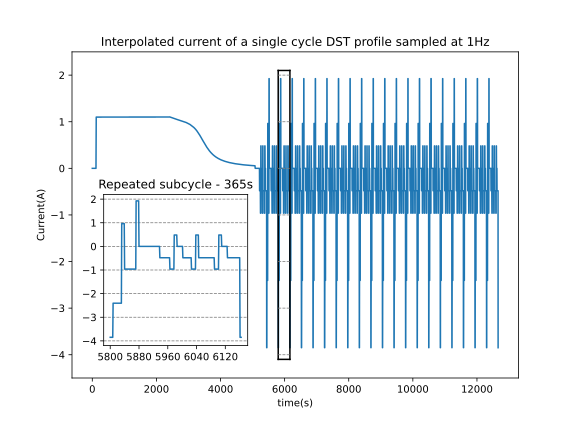
\includegraphics[width=6cm]{II_Body/images/Current-DST.png}
        \caption{\centering}
        \label{subfig:profs-DST}
    \end{subfigure}
    \vspace{1pc}
    \begin{subfigure}[b]{0.45\textwidth}
        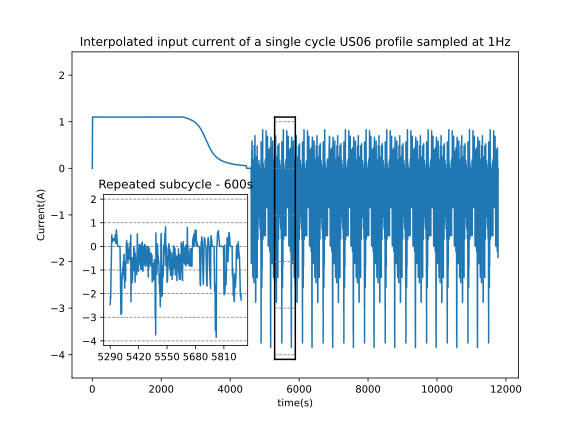
\includegraphics[width=6cm]{II_Body/images/Current-US06.png}
        \caption{\centering}
        \label{subfig:profs-US}
    \end{subfigure}
    \vspace{1pc}
    \begin{subfigure}[b]{0.45\textwidth}
        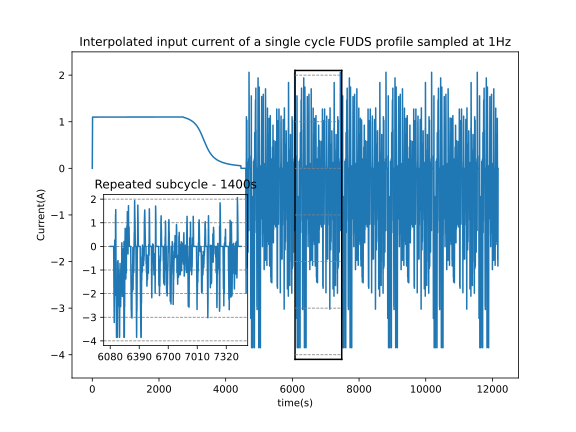
\includegraphics[width=6cm]{II_Body/images/Current-FUDS.png}
        \caption{\centering}
        \label{subfig:profs-FUDS}
    \end{subfigure}    
    %   \caption{\hl{Cell} %MDPI: please consider adding the descriptions for subfigures a--c in the main figure caption aswell. Please use commas to separate thousands for numbers with five or more digits (not for four digits) in the picture. e.g., "10000" should be "10,000
    %  Current
    %  of three battery testing profiles, emulating Constant-Current-Constant-Voltage charge and regenerative discharge until cells reached top or bottom cut-offs.}
    \caption{Cell current of three battery testing profiles, emulating a constant-current--constant-voltage charge and regenerative discharge until cells reached top or bottom cutoffs. (\textbf{a}) Dynamic stress test (DST) of 20 repeated subcycles; (\textbf{b}) highway driving schedule (US06) of 12 repeated subcycles; (\textbf{c})~federal urban driving schedule (FUDS) of 6 repeated subcycles.}
    \label{fig:current-profs}
\end{figure}

    \subsection{Model Training, Validation, and Testing Metrics Functions} \label{subsec:t_model}
%
% The evaluation process, how it is done and what it means to achieve
The evaluation procedures were conducted similarly to Mamo and \linebreak Wang's \cite{mamo_long_2020} research.
The same training, validation, and testing procedures were used to determine the best technique and performance.
%! Go more technical and complex
% Each training stage has been written from the first principle to focus on performance gain and implementation of published methods.
Each training stage was written from first principles using the CUDA-supported TensorFlow 2.3.1 framework's official documentation, with additional implementation to accommodate method modifications~\cite{chollet_writing_2020}.
This allowed a flexibility in modifying the training and evaluation procedures to come up with objective comparison criteria.
A single training iteration consisted of several stages, involving several performance and quality checks, to ensure that training improved until the optimum was achieved before hitting a limit.

% Save/load process to avoid overfitting early
%
Algorithm~\ref{alg:training} provides the pseudocode summary for the primary training procedures undertaken by every model.
Every training run worked with all three profiles, where the first cycle type was used for training and validation and another two for testing and performance rating, as illustrated in Figure~\ref{fig:cross-data}, with five charge/discharge cycles per type.
After a model setup, initial parameter definition, and a single-iteration (epoch) run with the entire training dataset, the models' mean average accuracy was compared with previous results to decide if retraining was necessary to foresee potential overfitting at Algorithm~\ref{alg:training} Line~\ref{alg:training-check}.
The interchange between different temperatures for validation was neglected to avoid unnecessary complexity in the comparison of the results.
If any improvement was observed, the model was saved as a checkpoint for a rollback if needed, before a follow-up evaluation, as in Algorithm~\ref{alg:training} Line~\ref{alg:training-succes}.
Otherwise, the model was rolled to the previous state and underwent another attempt, with a half-reduced current learning rate.
Within 3--8 attempts, the models recovered and continued learning with an error \mbox{between 3 and 6\%}, Algorithm~\ref{alg:training} Lines~\ref{alg:training-recovery-start} to~\ref{alg:training-recovery-end} as, after approximately 30--50 trials, they started to show obvious overfitting or underfitting results with no potential recovery.
The cycle-type train on Figure~\ref{fig:cross-data} demonstrates the one-to-five data breakdown between validation and training, where the cycle of 25 \textdegree{}C confirmed the general fitting process and produced an output for later use during performance averaging, as in Algorithm~\ref{alg:training} Line~\ref{alg:training-valid}.
For this investigation, a single-cycle verification at 25 \textdegree{}C was the primary criterion assessment, as per the research goal and limitations regarding the quantity of data that were provided.
Due to the potential assumption that a model inside an electric vehicle would undergo constant online learning, there was no situation when the model had to face completely unpredictable scenarios.
Finally, the model was tested against two other cycles types, as shown in Figure~\ref{fig:cross-data}, assessing the general state of charge cycling that was captured under different conditions, as in Algorithm~\ref{alg:training} Line~\ref{alg:training-test}.
Two cycles from 25 \textdegree{}C and 30 \textdegree{}C were selected as examples of the closest value ranges and most likely idle battery states.
The better the results, the more objective the model was in unseen conditions.
% An additional test against another battery takes place to verify the models' behaviour and the possibility for further improvement with new samples, which will not be part of performance measurements or discussion.
% The results from two other sample tests confirm that estimations are still rational within State of Charge behaviour boundaries.
If the model reached the optimum state, with no further accuracy improvements and hyperparameters to adjust, the training process was stopped and the model underwent the final evaluation against the entire training set with all three profiles, as in Algorithm~\ref{alg:training} Line~\ref{alg:training-end}.
%%%%%%%%%%%%%
\begin{algorithm}[H]%\captionsetup{labelfont={sc,bf}, labelsep=newline}
    \caption{Training procedure.}
    \begin{algorithmic}[1]
        \STATE Setup model. Define optimiser and metrics.
        \STATE Initialise parameters with initial learning rate at 0.001
        \STATE Set prev\_error 1
        \WHILE{epoch $<$ 100:}
            \STATE Train model, obtain gradients, and apply optimiser
            \IF{ error $>$ prev\_error:}  \label{alg:training-check}
                \WHILE{attempt $<$ 50:}
                    \STATE Load previous successful model \label{alg:training-recovery-start}
                    \STATE Reduce learning rate by half
                    \STATE Train model, obtain gradients, and apply optimiser
                    \IF{ error $<$ prev\_error:}
                        \STATE Update error. Save state. Break the loop. \label{alg:training-recovery-end}
                    \ENDIF
                \ENDWHILE
            \ELSE
                \STATE Update error. Save state. \label{alg:training-succes}
            \ENDIF
            \STATE Update learning rate based on the scheduler.
            \STATE Validate model on 25 \textdegree{}C cycler. \label{alg:training-valid}
            \STATE Test on two other profiles. \label{alg:training-test}
        \ENDWHILE
        \STATE Record overall results against entire training datasets. \label{alg:training-end}
    \end{algorithmic}
    \label{alg:training}
\end{algorithm}

% Accuracy evaluation explanation with drawings
%
% Testing performance gets measured against two cycles of each unsued scheduler using one of the available embedded devices capable of Machine Learning computation.
% The intention was to verify the model's capability to be used on low-power devices and still meet necessary performance requirements.
% The profile will be switched to another and perform the same training, validation and testing steps.
% This mechanism will output three models per method and nine figures outlining training and validation learning accuracies.
% Based on the progressive accuracy increase, a final iteration for this plot and discussion will be based on the lowest training and validation error.
The following process was adapted for all error calculations in training, verification, and testing.
Figure~\ref{fig:plot_demo} shows an example of the accuracy evaluation, where the actual state of charge is compared with the model's prediction.
The filled area below the plot captures the absolute error difference between two lines, as per Equation~(\ref{eq:abs-error}).
%%%%%%
The test procedure was performed on two cycles of each profile but at a different temperature to assess how perceptive the model was in capturing the average and high heat spikes that the battery module might experience.
Each result was summarised into a table and reported based on metrics values.
%%%%%%
\begin{equation}
    ABS error = \sqrt{(Actual-Prediction)^2}
    \label{eq:abs-error}
\end{equation}
%
%
% Finally, after completing all training, which results in 18 produced models, each will undertake an overall assessment.
% All outputs will be taken through the entire training set of three driving profiles from another cell, which was not part of the early training at all.
% It is expected that the lowest error will be against a dataset, which the model was trained on.
% That is why it was placed as a first record in the final comparison table.
% The report is based on the metrics, which were initially defined for training purposes.
% Following plot demonstrates how the multi-processing unit testing process is performed for all three driving profiles over a single model. 
%
% \subsubsection{Losses}~\label{subsub:losses}

%\mbox{Table~\ref{tab:experiment}} contains a separate column for every loss function, which has been applied to each tested model.
%Some equations were extracted directly from papers; others were written based on their definition and internal library implementation.
%The goal of the loss function is to calculate the error between model prediction and the actual value.
%The efficiencies and impact of each equation are hard to determine and are not the investigation's goal.
%The purpose of the table is only to provide the implementation references, which have been assumed during the programming of each published article-based model.
% \begin{table*}[htbp]
%     \renewcommand{\arraystretch}{1.3}
%     \caption{Model's loss functions}
%     \centering
%     \label{tab:losses}
%     \resizebox{\linewidth}{!}{
%     \begin{tabular}{ l l l c }
%         \hline\hline \\[-3mm]
%         Function Name & Method used in & Source articles & Equation \\ 
%         \hline
%         Absolute Error & & Song \textit{et al.}~\cite{song_lithium-ion_2018} & $|SoC_t-\hat{SoC_t}|$ \\
%         \hline
%         -- &\#1 \#4 & \makecell[l]{Chemal \textit{et al.}\cite{Chemali2017},\\Jiao \textit{et al.}~\cite{jiao_gru-rnn_2020}} & $\sum\limits^N_{t=0} \frac{1}{2} (SoC_t-\hat{SoC_t})^2$ \\
%         \hline
%         \makecell[l]{Mean Average\\ Percentage Error} &\#3 & Mamo \textit{et al.}~\cite{mamo_long_2020} & $\frac{100}{N}\sum\limits^N_{t=0}|\frac{SoC_t-\hat{SoC_t}}{SoC_t}|$ \\
%         \hline
%         -- &\#2 & Xiao \textit{et al.}~\cite{xiao_accurate_2019} & $\frac{\sum\limits^N_{t=1}(SoC_t-\hat{SoC_t})^2}{N}$ \\
%         \hline
%         \makecell[l]{Mean Average\\ Squared Error} &\#5 \#6 & \makecell[l]{Javid \textit{et al.}~\cite{javid_adaptive_2020},\\Zhang \textit{et al.}~\cite{zhang_deep_2020}} & $\sum\limits^N_{t=0} \sqrt{\frac{1}{n} (SoC_t-\hat{SoC_t})^2}$ \\
%         \hline\hline
%     \end{tabular}
%     }
% \end{table*}

% $ L = \sum\limits^N_{t=0} \frac{1}{2} (SoC_t-\hat{SoC_t})^2$ ~\cite{Chemali2017},~\cite{jiao_gru-rnn_2020} \\
% $ L = \sum\limits^N_{t=0} \sqrt{\frac{1}{n} (SoC_t-\hat{SoC_t})^2}$ ~\cite{javid_adaptive_2020}~\cite{zhang_deep_2020} \\
% $ L = (\sum\limits^N_{t=1}(SoC_t-\hat{SoC_t})^2)N$~\cite{xiao_accurate_2019} \\
% $ L = |SoC_t-\hat{SoC_t}|$ \\
% $ L = \frac{100}{N}\sum\limits^N_{t=0}|\frac{SoC_t-\hat{SoC_t}}{SoC_t}|$~\cite{mamo_long_2020} \\

% \ebd{table}
% $MAE = \frac{1}{N}\sum\limits^N_{t=1} |SoC_t-\hat{SoC_t}|$ \\
% $MAPE = \frac{100}{N}\sum\limits^N_{t=1}|\frac{SoC_t-\hat{SoC_t}}{SoC_t}|$ \\
% $RMSE = \sqrt{\frac{1}{N}\sum\limits^N_{t=1}(SoC_t-\hat{SoC_t})^2}$ \\
% $R^2 = 1-\frac{\sum\limits^N_{t=1}(SoC_t-\hat{SoC_t})^2}
%               {\sum\limits^N_{t=1}(SoC_t-M_{SoC})^2}$ - $M_{SoC}$ is the mean SoC \\
% $Error = \frac{SoC_t-\hat{SoC_5}}{SoC_t}$ - Not decided yet
% \subsubsection{Callbacks}
% For the stateless model, the method for resetting a State of the model has been derived with the Callback function of:
% Another Algorithm. \\
% \begin{lstlisting}[language=Python]
% class ResetCallback(tf.keras.callbacks.Callback):
%     reset_steps : int = 500
%     i_counter   : int = 0
%     def __init__(self):
%         self.i_counter = 0

%     def on_batch_begin(self, batch, logs=None):
%         if (self.i_counter % self.reset_steps) == 0:
%             self.model.reset_states()
%             self.i_counter = 0
%         self.i_counter += 1
% \end{lstlisting}
% \begin{enumerate}
%     \item Checkpoint saving only the best one based on smalest rmse
%     \item Tensorboard tmp folder
%     \item Early stopping is applyable
%     \item Procedure of training epoch by epoch or algorithm for offline and online.
% \end{enumerate}
% \subsubsection{Callbacks}
% \begin{itemize}
%     \item Checkpoint \\
%     \item Tensorboard \\
%     \item nanTerminate \\    
% \end{itemize}
% \subsubsection{Training and validation Loop??}
% \begin{itemize}
%     \item validation over what data? - single cycle \\
% \end{itemize}
% \subsubsection{Testing procedures??}
% \begin{itemize}
%     \item Converting model to the TF-Lite usage for TPU processor \\
%     \item 2 profiles - two cycle test \\
% \end{itemize}

%
%
% \subsubsection{Metrics}
% \textcolor{red}{Generally, Losses start form 0, metrics from 1. Articles which did overwise were assumed to be mistaken.}
% \textcolor{red}{Similar to loses and reasons why we have chosen those as our criteria.} \\

% Metrics functions used through out the research
%
%! References on who used.
%! varied metric used across articles, we will used 3.
Metrics functions acted as user evaluation criteria to assess the performance of the trained model during both fitting and validation processes.
Although some papers relied on different evaluation criteria, for this research, the metrics were unified, with several equations provided in \mbox{Table~\ref{tab:metrics}}.
%! >>>>>>>>>>>>>>>>>>>>>>>>>>>>>>>>> Response 3 - Point 8
\added[id=Responce 3]{The mean average error (MAE) and root-mean-square error (RMSE) are the two standard metric functions used in almost any machine-learning-related problem, whereas the coefficient of determination (R2), a measure of a model's goodness of fit, has been used in several sources; therefore, to be as complete and comparable as possible, this was also used as one of the comparison criteria in this article.
All metrics were used to represent the entire training and testing cycles, which could be interpreted as a meaningful overall quality of the fitting process.}
%! <<<<<<<<<<<<<<<<<<<<<<<<<<<<<<<<< Response 3 - Point 8
Thus, the same criteria were used to compare the model efficiencies.
\begin{figure}[ht]
    % \centering
    \includesvg[width=\textwidth]{II_Body/images/cross-data.svg}
    \caption{Three profiles cross data split for training, validation and testing in a simplistic SoC cycle representation through different temperatures}
    \label{fig:cross-data}
\end{figure}

\vspace{-18pt}

\begin{figure}[ht]
    % RMSE equation: RMS = (tf.keras.backend.sqrt(tf.keras.backend.square(y_test_one[::,]-PRED)))
    % \centering
    \includesvg[width=0.70\textwidth]{II_Body/images/plot-example.svg}
    \caption{Accuracy plot demonstration}
    \label{fig:plot_demo}
\end{figure}
\ifthenelse{\boolean{thesis}}{
\begin{table}[htbp]
    \renewcommand{\arraystretch}{1.3}
    \caption{Model's metrics functions}
    \centering
    \label{tab:metrics}
    \begin{tabular}{l c}
        \hline\hline \\[-3mm]
        Function Name & Equation \\ 
        \hline
        \makecell[l]{Mean Absolute\\ Error} &  $\frac{1}{N}\sum\limits^N_{t=1} |SoC_t-\hat{SoC_t}|$ \\
        % \hline
        % Mean Average Percentage Error & $\frac{100}{N}\sum\limits^N_{t=1}|\frac{SoC_t-\hat{SoC_t}}{SoC_t}|$ \\
        \hline
        \makecell[l]{Root Mean\\ Square Error} & $ \sqrt{\frac{1}{N}\sum\limits^N_{t=1} \left(SoC_t-\hat{SoC_t} \right)^2}$ \\
        \hline
        \makecell[l]{$R^2$ : $M_{SoC}$ is\\ the mean SoC} & $1-\frac{\sum\limits^N_{t=1}(SoC_t-\hat{SoC_t})^2}
                {\sum\limits^N_{t=1}(SoC_t-M_{SoC})^2}$ \\
        \hline\hline
        % Error : Not decided if useful yet & $ \frac{SoC_t-\hat{SoC_5}}{SoC_t}$
    \end{tabular}
\end{table}
}{
\begin{table}[H]
    \caption{Model's metrics functions.}
    \label{tab:metrics}
    \newcolumntype{C}{>{\centering\arraybackslash}X}
    \begin{tabularx}{\textwidth}{CC}
        \toprule
        \textbf{Function Name} & \textbf{Equation} \\
        \midrule
        Mean absolute error & $\frac{1}{N}\sum\limits^N_{t=1} |SoC_t-\hat{SoC_t}|$ \\
        \midrule
        Root-mean-square error & $ \sqrt{\frac{1}{N}\sum\limits^N_{t=1} \left(SoC_t-\hat{SoC_t} \right)^2}$ \\
        \midrule
        $R^2$ : $M_{SoC}$ is the mean SoC & $1-\frac{\sum\limits^N_{t=1}(SoC_t-\hat{SoC_t})^2}
        {\sum\limits^N_{t=1}(SoC_t-M_{SoC})^2}$ \\
        \bottomrule
    \end{tabularx}
\end{table}
}

% Concluding purpose of the training and ultimate goad of getting so creative
%
% Overall, the primary criteria of the research are the ability to fit the training data, avoiding overfits, constant reasonably short retraining potential, susceptibility to undetermined conditions and final memory and processing usage.
% Ultimately, all models will be compared with their successes and faults to determine a path for potential improvement.

    \subsection{Hyperparameters selection} \label{subsec:l-rate}
% Methods and their optimisers
%
%! Five stated models
The reviewed articles that the chosen models for testing were based on used constant hyperparameter values for models and optimisers, including learning rate.
However, each selected different values based on experiments and observations, somewhere in the range of 0.001 (the standard framework provided) down to 0.0001, to make a smooth stepping and minimise potentially missing the optimum minimum.
% A detailed overview of each method has been marked in \mbox{Table ~\ref{tab:experiment}}.

% Recovery from faults.
%
% Put a pseudo code for scheduler degradation.
% elif type == 'linear':
%   return linspace(0.001, 0.0001, 100)[epoch]
%   step = (stop - start) / (num - 1)
% for i in range(num):
%   yield start + step * i
% \begin{algorithm}\captionsetup{labelfont={sc,bf}, labelsep=newline}
%   \caption{Linear Scheduler implementation. Equivalent of \textit{linspace()} fn}
%   \begin{algorithmic}[1]
%     \STATE \textbf{Starting value} \\ $start\gets \textit{initial Learning rate}$\\
%     \STATE \textbf{End Value} \\ $stop\gets \textit{final Learning rate}$\\
%     \STATE \textbf{Number of iterations/Epochs} \\ $N = \textit{Epochs}$\\
%     \STATE \textbf{Calculate step between starting and end values, \\ including final learning rate} \\ $step = (stop - start) / (N - 1)$\\
%     \WHILE{$epoch \leq N$}
%     \STATE $\alpha \gets start + step * epoch$ \\ \COMMENT{Yield learning rate to an optimiser}
%     \ENDWHILE
%   \end{algorithmic}
%   \label{alg:scheduler}
% \end{algorithm}
% alpha_1 = alpha + delta
% Define delta degradation of learning rate
% Delta wash chosen to go from init to end. Decrement.
\begin{equation}
  \begin{split}
      IF \ AN \ & OVERFIT: \\
      \hat{\alpha} &= \frac{\alpha }{2} \\
      ELSE: & \\
      \Delta &= \frac{stop - start}{N-1} \\
      \hat{\alpha} &= \alpha + \Delta \times epoch \\
      \label{eq:scheduler}
  \end{split}
\end{equation}
\begin{figure}[ht]
    \centering
    \includesvg[width=\textwidth]{II_Body/images/l_rate.svg}
    \caption{Learning rate degradation}
    \label{fig:l_rate_progress}
\end{figure}
% As a result, a separate learning rate scheduler has been used instead of applying each learning rate separately for every model.
In this work, a stepping learning rate algorithm has been used for every optimiser over the training course, Equation~(\ref{eq:scheduler}).
The implementation is equivalent to a \textit{linspace} function, where every epoch's learning rate $\hat{\alpha}$ gets calculated through \textit{start} and \textit{stop} variables, indicating boundaries of the rates' degradation, with $\Delta$ decrement through a total of \textit{N} number of iterations inclusive, and known $\alpha$ value.
%
% Like adaptive time stepping in Finite Element Analysis [ref] by Pr David Holmes
The learning rate is sequentially reduced following a standard stepped scheme.
However, an additional adaptive phase is introduced in this work.
While training error in subsequent epochs reduces, the stepped scheme is followed.
The adaptive scheme is deployed if the learning error increases from one epoch into the next.
Then, the rate is halved, and the same epoch is rerun.
If the training error remains above the error of the previous epoch, the learning rate continues to be reduced to a predetermined minimum.
The prior stepped scheme resumes if the error returns to a convergent value.
It is shown in Figure~\ref{fig:l_rate_progress}, where two adaptive schemes are applied and reconverged from, and a final ultimate adaptive decay ends the training.
%
This approach has been found to be superior in this work to other adaptive learning rate schemes, and is employed for all subsequent training.
%
% However, continuous learning rate reduction does not resolve the issue of overfitting or missing a minimum.
% The best approach identified in this work to save time and produce reliable results has been to enforce a model to stick toward a single minimum.
% In this case, the learning rate always follows the stick degradation curve as per Figure~\ref{fig:l_rate_progress}, without affecting the follow-up training with steep rate reduction upon failures.
% Since each model undergoes multiple attempts, there are good chances to explore a variety of different fitting scenarios rather than jumping between several minimal.
% Two subfigures on \mbox{Figure~\ref{fig:rollback}} demonstrate two different training attempts with and without a recovery algorithm.
% While subfigure~\ref{subfig:no-rollback} keeps the training process until either the number of 100 epochs gets reached or rapid overfit, the subfigure~\ref{subfig:no-rollback} continues reaching the selected minimal for as long as it can achieve a result.
% Considering that all attempts to train the estimator eventually tended to overfit, the learning rate's value has been reduced by half each time model recovers from overshoot, Equation~\ref{eq:scheduler}.
% Epochs 26 and further indicate the training attempt to recover from the overfitting state on an LSTM model, reducing the rate in several dozen attempts, never reaching zero.
% Once the model fails to improve the accuracy, it is considered the most optimum fit to initiate early stopping.
\begin{figure}[htbp]
  \centering
  \begin{subfigure}[b]{0.45\textwidth}
      \centering
      \includesvg[width=\linewidth]{II_Body/images/history-bad.svg}
      \caption{Model training process with no rollbacks \\ }
      \label{subfig:no-rollback}
  \end{subfigure}
  \hfill
  \begin{subfigure}[b]{0.45\textwidth}
      \centering
      \includesvg[width=\linewidth]{II_Body/images/history-good.svg}
      \caption{Model training process with a rollback if current error higher than previous}
      \label{subfig:rollback}
  \end{subfigure}
  \caption{Training process comparison with and without having a recovery algorithm}
  \label{fig:rollback}
\end{figure}

% Betas and Epsilon instead on every optimiser page
%
The betas and epsilon optimisers' constants did not go through any similar optimisation process due to a lack of documented training attempts to improve fitting over State of Charge estimation on Lithium-Ion batteries.
As a result, they were kept constant for all trained models except SGDw/M.
Since Stochastic Gradient Descent does not use any other hyper-parameters except the learning rate and the single beta constant, its value was set to $\beta_1 = 0.8$.
The learning rate limits of the scheduler and remaining hyperparameters used in all cases are summarised in \mbox{Table~\ref{tab:uni-hyperparams}}.
\ifthenelse{\boolean{thesis}}{
\begin{table}[htbp]
  \renewcommand{\arraystretch}{1.3}
  \caption{Optimiser Hyper-Parameters}
  \centering
  \label{tab:uni-hyperparams}
  \begin{tabular}{ l l l l l l }
      \hline\hline \\[-3mm]
      $\alpha$ & $\beta_1 $ & $\beta_2$ & $\beta_3$ &  $\epsilon$ \\
      \hline
      Linear         &  &  &  & \\% 0.0000001
      Scheduler      & $0.9$ & $0.999$ & $0.999$ &$10^{-8}$ \\% 0.0000001
      (0.001-0.0001) &  &  &  & \\% 0.0000001
      \hline\hline
  \end{tabular}
\end{table}
} {
\begin{table}[H]
  \caption{Optimiser Hyper-Parameters}
  \label{tab:uni-hyperparams}
  \newcolumntype{C}{>{\centering\arraybackslash}X}
  \begin{tabularx}{\textwidth}{ C C C C C C }
    \toprule
    \textbf{$\alpha$} & \textbf{$\beta_1 $} & \textbf{$\beta_2$} & \textbf{$\beta_3$} &  \textbf{$\epsilon$} \\
    \midrule
    Linear         &  &  &  & \\% 0.0000001
    Scheduler      & $0.9$ & $0.999$ & $0.999$ &$10^{-8}$ \\% 0.0000001
    (0.001-0.0001) &  &  &  & \\% 0.0000001
    \bottomrule
  \end{tabularx}
\end{table}
}
% Layers and neurons
%
The work performed by other authors from Table~\ref{tab:review} uses a constant number of layers and neurons to conduct the experiments.
Only a few have provided reasoning for the selections or results from other attempted experiments without changing the technique~\cite{jiao_gru-rnn_2020,mamo_long_2020}.
The least time-consuming method evaluated the most promising combination of the number of layers and neurons to create the best similar circumstances for all methods.
The most promising candidates were taken through a dozen similar attempts to get an average result, and produce several selection criteria for later use.

    \subsection{Results averaging} \label{subsec:avg}
% Stochastic nature of ML and Averaging 
%
%* Most deep learning algorithms are based on an optimization algorithm called stochastic gradient descent. — Page 98, Deep Learning, 2016.
The five models used in this research had a stochastic nature due to the use of randomness in the  gradient calculation during the learning~\cite{alma991010036879604001}, such as the stochastic gradient descent, which is discussed in Section~\ref{subsec:optimisers}.
As such, obtaining repeatable results which were worth comparing required the implementation of an averaging method, in which each model undertook the same procedures multiple times.
The resulting plots and values provided far more representative statistical criteria, as opposed to random fluctuations.
% \textcolor{red}{5 ML is stochastict thongs. As such, to get repeatable you need to account for statistics, to account, we have implemented averaging methods, where each model is trained 10 times and results averaged to provide significant statistical criteria (representative) as opposed to random fluctuations/
%As an example of this method FUDS has been used, showing a spread....}

% Average 10 attempts with accuracy calculus.
%
During preliminary work, this research attempted to train many models of the same type to produce the best-fitting line.
%Due to MLs' stochastic nature,
The training results showed a significant variance.
As such, training was repeated ten times for each dataset to remove the statistical variance from the comparison results, and the average of all ten trained models was used in each result.
Figures~\ref{fig:Model-DEMO} and~\ref{fig:Model-DEMO2} show this process, where Figures \ref{fig:Model-DEMO}a and \ref{fig:Model-DEMO2}a show a single test training history and final SoC prediction, Figures \ref{fig:Model-DEMO}b and \ref{fig:Model-DEMO2}b show the spread of 10 similar training sessions, and Figures \ref{fig:Model-DEMO}c and \ref{fig:Model-DEMO2}c show the averaged result.
It is apparent that, while some repeats were highly accurate, others had more significant errors, see Figure~\ref{fig:Model-DEMO}b.
The averaging provided a representative, statistically repeatable result.
% similar to Subfigure~\ref{subfig:Model-DEMO-10} and ~\ref{subfig:Model-DEMO2-10}.
% The Earliest attempt to unify all models was the application of the same set seed number for all models.
% However, determining a case from an infinite number of possibilities to produce equally effective models is the least effective method.
% Therefore, an average result of multiple attempts to smoothen history and SoC prediction curves has been introduced.
% Figures~\ref{fig:Model-DEMO} and~\ref{fig:Model-DEMO2} represent the difference between single and multiple averaged models and the general spread.
% Subfigure~\ref{subfig:Model-DEMO-10} demonstrates how ten different models, each potentially minimised toward a single minimal, get spread from each other, producing variable results.
% Similar case with SoC prediction on Subfigure~\ref{subfig:Model-DEMO2-10}, where combined predictions and RMS highlight potential inefficancies in the prediction of the same task 
% Subfigures~\ref{subfig:Model-DEMO-1} and~\ref{subfig:Model-DEMO-avr} show a comparison between randomly selected single and averaged model history results.
% Whereas Subfigures~\ref{subfig:Model-DEMO2-1} and~\ref{subfig:Model-DEMO2-avr} outline that the best case does bring subjective results to the efficiency of the techniques in terms of accurate results.
% Due to the most trendiness plots and apparent convergence or divergence inclination, the method has proven to be the most objective result.
% \textit{NaN} values were ignored in the cases of prolonged history.
% The same method has been applied to all SoC plots for all models, reported further.
%Several evaluation possibilities were tested. In the end, an average of 10 provided the most objective results to overview.
%\textcolor{red}{Show plot of 1, then all 10 and average took.}
\begin{figure}[H]
    % \centering
    \begin{subfigure}[b]{0.325\textwidth}
        % \centering
        \includesvg[width=4.5cm]{III_Conclussion/Results_new/DEMO1-history-FUDS-mae.svg}
        \caption{\centering}
        \label{subfig:Model-DEMO-1}
    \end{subfigure}
    % \hfill
    \begin{subfigure}[b]{0.325\textwidth}
        % \centering
        \includesvg[width=4.5cm]{III_Conclussion/Results_new/DEMO2-history-FUDS-mae.svg}
        \caption{\centering}
        \label{subfig:Model-DEMO-10}
    \end{subfigure}
    % \hfill
    \begin{subfigure}[b]{0.325\textwidth}
        % \centering
        \includesvg[width=4.5cm]{III_Conclussion/Results_new/DEMO3-history-FUDS-mae.svg}
        \caption{\centering}
        \label{subfig:Model-DEMO-avr}
    \end{subfigure}
    \caption{History results averaging demonstration. (\textbf{a}) Single model history for training and testing; (\textbf{b}) All 10 attempts of histories for training and testing; (\textbf{c}) Average of 10 attempts of histories for training and testing.}
    \label{fig:Model-DEMO}
\end{figure}
\begin{figure}[H] %Attention AE: please change SoC(%) to SoC (%).
    % \centering
    \begin{subfigure}[b]{0.325\textwidth}
        % \centering
        \includesvg[width=4.5cm]{III_Conclussion/Results_new/DEMO1-SoC-FUDS.svg}
        \caption{\centering}
        \label{subfig:Model-DEMO2-1}
    \end{subfigure}
    %\hfill
    \begin{subfigure}[b]{0.325\textwidth}
        % \centering
        \includesvg[width=4.5cm]{III_Conclussion/Results_new/DEMO2-SoC-FUDS.svg}
        \caption{\centering}
        \label{subfig:Model-DEMO2-10}
    \end{subfigure}
    % \hfill
    \begin{subfigure}[b]{0.325\textwidth}
        % \centering
        \includesvg[width=4.5cm]{III_Conclussion/Results_new/DEMO3-SoC-FUDS.svg}
        \caption{\centering}
        \label{subfig:Model-DEMO2-avr}
    \end{subfigure}
    \caption{State of charge results' averaging demonstration. (\textbf{a}) Single-model SoC prediction for training; (\textbf{b}) all 10 attempts a SoC prediction on a single plot; (\textbf{c}) average of 10 attempts at SoC prediction for training.}
    \label{fig:Model-DEMO2}
\end{figure}

%
%
\ifthenelse{\boolean{thesis}}{
    In the next Section~\ref{sec:AN:Results}, first tests to determine optimum hyperparameters are discussed; then, the full evaluation of models against each of the drive cycles is presented.
} {
    In the next Section~\ref{sec:results}, the first tests carried out to determine the optimum hyperparameters are discussed; then, the full evaluation of models against each of the drive cycles is presented.
    In each case, the train/validation/test procedures and error metrics of \mbox{Section~\ref{subsec:t_model}} were followed, with the learning rate method in Section~\ref{subsec:l-rate} and an average of 10 training sessions as in Section~\ref{subsec:avg} to ensure the best and most accurate representation of each model.
}
    % \subsection{Hardware and Software} \label{subsec:soft}
% This subsection will outline hardware and software details used in the research process.
% It intended to provide necessary outlines to support further research and allow repeating the experiment with different conditions.

% Embedded devices for performance measurements
%
Three devices acted as embedded computing test units in different hardware and computational levels: Tensor Processing Unit (TPU), Raspberry Pi 4 (R-Pi4), and an Android-based smartphone.
Coral TPU produced by Google has limited specifications information, but the software has provided two libraries for average and maximum clock frequency computation.
Raspberry Pi 4 is powered with Quad-core Cortex-A72 (ARM v8) and 2GB RAM.
The Operating System was selected with a beta version of Raspbian 64 (aarch64).
The selection of Android devices depended on the highest percentage distribution.
An Octa-core Cortex-A53 with 3GB RAM seemed the most commonly used at the time.
The inbuilt chipset is Mediatek MT6753 (28 nm) with Android version 6.

% Model training Framework
%
The framework for Machine Learning has been Tensorflow 2.4.0 with Python 3.9.1 compiled from source using Bazel 3.1.0.
An additional package with Addons 0.18 for $R^2$ and Probability 0.13 for Differential Evoltions algorithms has been compiled from the source and added to the main framework.
Tensorboard is used to observe progress and keep records to analyse training later. It also made an excellent initial tool for model profiling and performance measure.

% Final performance tests
%
End of the training testing of each model has been performed on the Coral TPU device with TensorFlow-Lite Runtime library version 2.5.0.
Every model has been trained and converted to its' TFLite version to validate the ability to be suitable for deployment.
At the current stage and version of the TensorFlow, the Stateful models have not been supported for lite version conversion.
Final model testing against the entire set of all three profiles has been performed on a desktop machine with an Intel CPU and two Graphical Processors with Compute Capability Score of 7.5.
The version of the CUDA library for GPU computation that has been used is 11.1 from the beginning of the research.
%
% IF
\ifthenelse {\boolean{thesis}}
%
% THEN
{
\mbox{Figure~\ref{fig:device_compute}} demonstrates the paralysation mechanism for a single model, where flops and the total number of parameters are determined using the script in Appendix~\ref{app:flops}.
}
{
\mbox{Figure~\ref{fig:device_compute}} demonstrates the paralysation mechanism for a single model version final testing, with three trained versions for each profile.
}
\begin{figure}[ht]
    \centering
    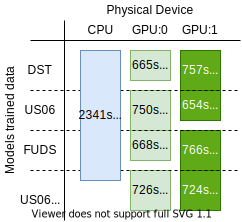
\includegraphics[width=\columnwidth]{II_Body/images/Accuracy_Compute.png}
    % \includesvg[width=\linewidth]{II_Body/images/Accuracy_Compute_10.svg}
    \caption{Accuracy computation using a single model trained on different proflies separately. The timing examples were taken from Model \#5 computation process.}
    \label{fig:device_compute}
\end{figure}
%
% Attention Layer has been reimplemented from provided source code.%\textcolor{red}{Good luck finding the link}
% Robust Adam was also implemented from the source; what should I do with that now?
% Multilayer model flagged with Return sequences boolean. Statefulnes define with Stateful boolean. The dropout is affected as a separate layer or parameter. With Stateful on, standard Input Layer shape requires to be follower Bacthed Input shape. It can be done kwarg parameter to the GRU or LSTM layer or kept as a separate Input Layer to allow precompilation before starting model fitting. Following code, the snipest demonstrated the difference. 

% \textcolor{red}{I am going to use the TPU processor to measure time it takes to run e ach model.} \\
% \begin{table}[ht]
%     \centering
%     \caption{Software details}
%     \label{tab:my_label}
%     \begin{tabular}{p{3.0cm}|c|c|c|c|c}
%         Version & Python version & Compiler & Build tools & CUDA version & Compute Score\\
%         Tensorflow-2.4.0, TF-Addons 13.0, TF-Probability 0.12.1 & 3.9.1 & gcc 9.3.0 & Bazel 3.1.0 & 11.1 & 7.5\\
%         \hline
%         Tensorflow-2.2.0 & 3.8.* & gcc 7.3.1 & Bazel 2.0.0 & CPU & 3.98MHz*
%     \end{tabular}
% \end{table}



%Table information collected as per datasheet. \\
%Android device: 3GB - RAM, Octa-core 1.3 GHz Cortex-A53, Android 5.1 (6), Chipset: Mediatek MT6753 (28 nm), \\

%GFLOPS table: http://web.eece.maine.edu/~vweaver/group/green_machines.html

% R-Pi3B as per Tim Chant:
% 70.45 GFLOPS / 6.2 GFLOPS/s = 11.36 s
% Total model flops / device flops = Time  --->>>>> Time * Device flops = Total model flops

% Energy consumption if Voltage and Current from device records not enough
% 1.36 s/s * 3.7 W / 3,600s = 0.0116 Wh/s


% \begin{table}[]
%     \centering
%     \caption{Chip-on-Board Hardware selection}
%     \label{tab:my_label}
%     \begin{tabular}{c|c|c|c}
%         Device & Specification & Source & Software setup \\
%         \hline
%         Coral TPU & (Specs) & (Link to the details) & (Link to libedgetpu.so.1) \\
%         \hline
%         Raspberry Pi 4 (Active cooling) & 
%     \end{tabular}
% \end{table}    %! Hardware goes to the thesis
%%%%%%%%%%%%%%%%%%%%%%%%%%%%%%%%%%%%%%%%%%
%%% Results
\section{Performance and Results}\label{sec:results}
%%% %%%%%%%%%%%%%%%%%%%%%%%%%%%%%%%%%%%%%%%%%%%%%%%%%%%
%%%%%%%%%%%%%% Model \#1 Chemali2017 %%%%%%%%%%%%%%%
\begin{figure*}[htbp]
    \centering
    \begin{subfigure}[b]{0.95\textwidth}
        \centering
        \includesvg[width=\linewidth]{III_Conclussion/Results/Models/Chemali2017/DST-models/Chhistory-DST.svg}
        \caption{DST - Training accuracy history}
    \end{subfigure}
    \hfill
    \begin{subfigure}[b]{0.95\textwidth}
        \centering
        \includesvg[width=\linewidth]{III_Conclussion/Results/Models/Chemali2017/US06-models/Chhistory-US06.svg}
        \caption{US06 - Training accuracy history}
    \end{subfigure}
    \hfill
    \begin{subfigure}[b]{0.95\textwidth}
        \centering
        \includesvg[width=\linewidth]{III_Conclussion/Results/Models/Chemali2017/FUDS-models/Chhistory-FUDS.svg}
        \caption{FUDS Training accuracy history}
    \end{subfigure}    
    \caption{Model 1: Single Layer Stateless LSTM Losses}
    \label{fig:Model-1losses}
\end{figure*}
% %%%%%%%%%%%%%% Model \#2 BinXiao2020 %%%%%%%%%%%%%%%
% \begin{figure*}[htbp]
%     \centering
%     \begin{subfigure}[b]{0.95\textwidth}
%         \centering
%         \includesvg[width=\linewidth]{III_Conclussion/Results/Models/BinXiao2020/DST-models/Bihistory-DST.svg}
%         \caption{DST - Training accuracy history}
%     \end{subfigure}
%     \hfill
%     \begin{subfigure}[b]{0.95\textwidth}
%         \centering
%         \includesvg[width=\linewidth]{III_Conclussion/Results/Models/BinXiao2020/US06-models/Bihistory-US06.svg}
%         \caption{US06 - Training accuracy history}
%     \end{subfigure}
%     \hfill
%     \begin{subfigure}[b]{0.95\textwidth}
%         \centering
%         \includesvg[width=\linewidth]{III_Conclussion/Results/Models/BinXiao2020/FUDS-models/Bihistory-FUDS.svg}
%         \caption{FUDS Training accuracy history}
%     \end{subfigure}    
%     \caption{Model 2: Single Layer Stateless GRU Losses.}
%     \label{fig:Model-2losses}
% \end{figure*}
% %%%%%%%%%%%% Model \#3 TadeleMamo2020 %%%%%%%%%%%%%%
% \begin{figure*}[htbp]
%     \centering
%     \begin{subfigure}[b]{0.95\textwidth}
%         \centering
%         \includesvg[width=\linewidth]{III_Conclussion/Results/Models/TadeleMamo2020/DST-models/Tahistory-DST.svg}
%         \caption{DST - Training accuracy history}
%     \end{subfigure}
%     \hfill
%     \begin{subfigure}[b]{0.95\textwidth}
%         \centering
%         \includesvg[width=\linewidth]{III_Conclussion/Results/Models/TadeleMamo2020/US06-models/Tahistory-US06.svg}
%         \caption{US06 - Training accuracy history}
%     \end{subfigure}
%     \hfill
%     \begin{subfigure}[b]{0.95\textwidth}
%         \centering
%         \includesvg[width=\linewidth]{III_Conclussion/Results/Models/TadeleMamo2020/FUDS-models/Tahistory-FUDS.svg}
%         \caption{FUDS Training accuracy history}
%     \end{subfigure}    
%     \caption{Model 3: Single Layer Stateless LSTM with Attention Losses}
%     \label{fig:Model-3losses}
% \end{figure*}
% %%%%%%%%%%%%% Model \#$4 MengJiao2020 %%%%%%%%%%%%%%
% \begin{figure*}[htbp]
%     \centering
%     \begin{subfigure}[b]{0.95\textwidth}
%         \centering
%         \includesvg[width=\linewidth]{III_Conclussion/Results/Models/MengJiao2020/DST-models/Mehistory-DST.svg}
%         \caption{DST - Training accuracy history}
%     \end{subfigure}
%     \hfill
%     \begin{subfigure}[b]{0.95\textwidth}
%         \centering
%         \includesvg[width=\linewidth]{III_Conclussion/Results/Models/MengJiao2020/d_US06-models/Mehistory-d_US06.svg}
%         \caption{US06 - Training accuracy history}
%     \end{subfigure}
%     \hfill
%     \begin{subfigure}[b]{0.95\textwidth}
%         \centering
%         \includesvg[width=\linewidth]{III_Conclussion/Results/Models/MengJiao2020/d_FUDS-models/Mehistory-d_FUDS.svg}
%         \caption{FUDS Training accuracy history}
%     \end{subfigure}    
%     \caption{Model 4: Two Layer Stateful GRU Losses}
%     \label{fig:Model-4losses}
% \end{figure*}
% %%%%%%%%%%% Model \#5 GelarehJavid2020 %%%%%%%%%%%%%
% \begin{figure*}[htbp]
%     \centering
%     \begin{subfigure}[b]{0.95\textwidth}
%         \centering
%         \includesvg[width=\linewidth]{III_Conclussion/Results/Models/GelarehJavid2020/DST-models/Gehistory-DST.svg}
%         \caption{DST - Training accuracy history}
%     \end{subfigure}
%     \hfill
%     \begin{subfigure}[b]{0.95\textwidth}
%         \centering
%         \includesvg[width=\linewidth]{III_Conclussion/Results/Models/GelarehJavid2020/US06-models/Gehistory-US06.svg}
%         \caption{US06 - Training accuracy history}
%     \end{subfigure}
%     \hfill
%     \begin{subfigure}[b]{0.95\textwidth}
%         \centering
%         \includesvg[width=\linewidth]{III_Conclussion/Results/Models/GelarehJavid2020/FUDS-models/Gehistory-FUDS.svg}
%         \caption{FUDS Training accuracy history}
%     \end{subfigure}    
%     \caption{Model 5: Single Layer Stateless GRU Losses}
%     % -  \textcolor{red}{Error with RMS. Most likely the order of the root and mean has been flipped. Probably will require entire retraining to determine new measurments. Shape it was done long ago, there are no so detailed logs.}
%     %! NOTE: THis is a new version, retrained from the beginning. All remaining plots and data were kept from previos one, only the error curse was remade to fix RMSE 
%     \label{fig:Model-5losses}
% \end{figure*}
% %%%%%%%%%%%%% Model \#6 WeiZhang2020 %%%%%%%%%%%%%%%
% \begin{figure*}[htbp]
%     \centering
%     \begin{subfigure}[b]{0.95\textwidth}
%         \centering
%         \includesvg[width=\linewidth]{III_Conclussion/Results/Models/WeiZhang2020/DST-models/Wehistory-DST.svg}
%         \caption{DST - Training accuracy history}
%     \end{subfigure}
%     \hfill
%     \begin{subfigure}[b]{0.95\textwidth}
%         \centering
%         \includesvg[width=\linewidth]{III_Conclussion/Results/Models/WeiZhang2020/US06-models/Wehistory-US06.svg}
%         \caption{US06 - Training accuracy history}
%     \end{subfigure}
%     \hfill
%     \begin{subfigure}[b]{0.95\textwidth}
%         \centering
%         \includesvg[width=\linewidth]{III_Conclussion/Results/Models/WeiZhang2020/FUDS-models/Wehistory-FUDS.svg}
%         \caption{FUDS Training accuracy history}
%     \end{subfigure}    
%     \caption{Model 6: - Two Layer Stateless GRU Losses}
%     \label{fig:Model-6losses}
% \end{figure*}

%%% %%%%%%%%%%%%%%%%%%%%%%%%%%%%%%%%%%%%%%%%%%%%%%%%%%
%%%%%%%%%%%%% Model \#1 Chemali2017 %%%%%%%%%%%%%%%
%%%%%%%%%%%%%%%%%%%%%%%%%%%%%%%%%%%%%%%%%%%%%%%%%%
\begin{figure*}[htbp]
    \centering
    %%%%%%%%%%%%%%%%% DST based tests %%%%%%%%%%%%%%%%%
    \begin{subfigure}[b]{0.325\textwidth}
        \centering
        \includesvg[width=\linewidth]{III_Conclussion/Results/Models/Chemali2017/DST-models/ChDST-val-45.svg}
        \caption{Validated on DST}
    \end{subfigure}
    \hfill
    \begin{subfigure}[b]{0.325\textwidth}
        \centering
        \includesvg[width=\linewidth]{III_Conclussion/Results/Models/Chemali2017/DST-models/ChDST-Test One-45.svg}
        \caption{Tested on US06}
    \end{subfigure}
    \hfill
    \begin{subfigure}[b]{0.325\textwidth}
        \centering
        \includesvg[width=\linewidth]{III_Conclussion/Results/Models/Chemali2017/DST-models/ChDST-Test Two-45.svg}
        \caption{Tested on FUDS}
    \end{subfigure}
    %%%%%%%%%%%%%%%%% US06 based tests %%%%%%%%%%%%%%%%%
    \begin{subfigure}[b]{0.325\textwidth}
        \centering
        \includesvg[width=\linewidth]{III_Conclussion/Results/Models/Chemali2017/US06-models/ChUS06-val-50.svg}
        \caption{Validated on US06}
    \end{subfigure}
    \hfill
    \begin{subfigure}[b]{0.325\textwidth}
        \centering
        \includesvg[width=\linewidth]{III_Conclussion/Results/Models/Chemali2017/US06-models/ChUS06-Test One-50.svg}
        \caption{Tested on DST}
    \end{subfigure}
    \hfill
    \begin{subfigure}[b]{0.325\textwidth}
        \centering
        \includesvg[width=\linewidth]{III_Conclussion/Results/Models/Chemali2017/US06-models/ChUS06-Test Two-50.svg}
        \caption{Tested on FUDS}
    \end{subfigure}
    %%%%%%%%%%%%%%%%% FUDS based tests %%%%%%%%%%%%%%%%%
    \begin{subfigure}[b]{0.325\textwidth}
        \centering
        \includesvg[width=\linewidth]{III_Conclussion/Results/Models/Chemali2017/FUDS-models/ChFUDS-val-48.svg}
        \caption{Validated on FUDS}
    \end{subfigure}
    \hfill
    \begin{subfigure}[b]{0.325\textwidth}
        \centering
        \includesvg[width=\linewidth]{III_Conclussion/Results/Models/Chemali2017/FUDS-models/ChFUDS-Test One-48.svg}
        \caption{Tested on DST}
    \end{subfigure}
    \hfill
    \begin{subfigure}[b]{0.325\textwidth}
        \centering
        \includesvg[width=\linewidth]{III_Conclussion/Results/Models/Chemali2017/FUDS-models/ChFUDS-Test Two-48.svg}
        \caption{Tested on US06}
    \end{subfigure}
    \caption{Model 1: Single Layer Stateless LSTM.\textbf{DO NOT FORGET TO RECOMPUTE THOSE PLOTS. AGAIN!!!}}
    \label{fig:Model-1res}
\end{figure*}
\clearpage
% %%%%%%%%%%%%%%%%%%%%%%%%%%%%%%%%%%%%%%%%%%%%%%%%%%%
% %%%%%%%%%%%%%% Model \#2 BinXiao2020 %%%%%%%%%%%%%%%
% %%%%%%%%%%%%%%%%%%%%%%%%%%%%%%%%%%%%%%%%%%%%%%%%%%%
% \begin{figure*}[htbp]
%     \centering
%     %%%%%%%%%%%%%%%%% DST based tests %%%%%%%%%%%%%%%%%
%     \begin{subfigure}[b]{0.325\textwidth}
%         \centering
%         \includesvg[width=\linewidth]{III_Conclussion/Results/Models/BinXiao2020/DST-models/BXDST-val-50.svg}
%         \caption{Validated on DST}
%     \end{subfigure}
%     \hfill
%     \begin{subfigure}[b]{0.325\textwidth}
%         \centering
%         \includesvg[width=\linewidth]{III_Conclussion/Results/Models/BinXiao2020/DST-models/BXDST-Test One-50.svg}
%         \caption{Tested on US06}
%     \end{subfigure}
%     \hfill
%     \begin{subfigure}[b]{0.325\textwidth}
%         \centering
%         \includesvg[width=\linewidth]{III_Conclussion/Results/Models/BinXiao2020/DST-models/BXDST-Test Two-50.svg}
%         \caption{Tested on FUDS}
%     \end{subfigure}
%     %%%%%%%%%%%%%%%%% US06 based tests %%%%%%%%%%%%%%%%%
%     \begin{subfigure}[b]{0.325\textwidth}
%         \centering
%         \includesvg[width=\linewidth]{III_Conclussion/Results/Models/BinXiao2020/US06-models/BXUS06-val-50.svg}
%         \caption{Validated on US06}
%     \end{subfigure}
%     \hfill
%     \begin{subfigure}[b]{0.325\textwidth}
%         \centering
%         \includesvg[width=\linewidth]{III_Conclussion/Results/Models/BinXiao2020/US06-models/BXUS06-Test One-50.svg}
%         \caption{Tested on DST}
%     \end{subfigure}
%     \hfill
%     \begin{subfigure}[b]{0.325\textwidth}
%         \centering
%         \includesvg[width=\linewidth]{III_Conclussion/Results/Models/BinXiao2020/US06-models/BXUS06-Test Two-50.svg}
%         \caption{Tested on FUDS}
%     \end{subfigure}
%     %%%%%%%%%%%%%%%%% FUDS based tests %%%%%%%%%%%%%%%%%
%     \begin{subfigure}[b]{0.325\textwidth}
%         \centering
%         \includesvg[width=\linewidth]{III_Conclussion/Results/Models/BinXiao2020/FUDS-models/BXFUDS-val-50.svg}
%         \caption{Validated on FUDS}
%     \end{subfigure}
%     \hfill
%     \begin{subfigure}[b]{0.325\textwidth}
%         \centering
%         \includesvg[width=\linewidth]{III_Conclussion/Results/Models/BinXiao2020/FUDS-models/BXFUDS-Test One-50.svg}
%         \caption{Tested on DST}
%     \end{subfigure}
%     \hfill
%     \begin{subfigure}[b]{0.325\textwidth}
%         \centering
%         \includesvg[width=\linewidth]{III_Conclussion/Results/Models/BinXiao2020/FUDS-models/BXFUDS-Test Two-50.svg}
%         \caption{Tested on US06}
%     \end{subfigure}
%     \caption{Model 2: Single Layer Stateless GRU}
%     \label{fig:Model-2res}
% \end{figure*}
% \clearpage
% %%%%%%%%%%%%%%%%%%%%%%%%%%%%%%%%%%%%%%%%%%%%%%%%%%%
% %%%%%%%%%%%% Model \#3 TadeleMamo2020 %%%%%%%%%%%%%%
% %%%%%%%%%%%%%%%%%%%%%%%%%%%%%%%%%%%%%%%%%%%%%%%%%%%
% \begin{figure*}[htbp]
%     \centering
%     %%%%%%%%%%%%%%%%% DST based tests %%%%%%%%%%%%%%%%%
%     \begin{subfigure}[b]{0.325\textwidth}
%         \centering
%         \includesvg[width=\linewidth]{III_Conclussion/Results/Models/TadeleMamo2020/DST-models/TMDST-val-19.svg}
%         \caption{Validated on DST}
%     \end{subfigure}
%     \hfill
%     \begin{subfigure}[b]{0.325\textwidth}
%         \centering
%         \includesvg[width=\linewidth]{III_Conclussion/Results/Models/TadeleMamo2020/DST-models/TMDST-Test One-19.svg}
%         \caption{Tested on US06}
%     \end{subfigure}
%     \hfill
%     \begin{subfigure}[b]{0.325\textwidth}
%         \centering
%         \includesvg[width=\linewidth]{III_Conclussion/Results/Models/TadeleMamo2020/DST-models/TMDST-Test Two-19.svg}
%         \caption{Tested on FUDS}
%     \end{subfigure}
%     %%%%%%%%%%%%%%%%% US06 based tests %%%%%%%%%%%%%%%%%
%     \begin{subfigure}[b]{0.325\textwidth}
%         \centering
%         \includesvg[width=\linewidth]{III_Conclussion/Results/Models/TadeleMamo2020/US06-models/TMUS06-val-25.svg}
%         \caption{Validated on US06}
%     \end{subfigure}
%     \hfill
%     \begin{subfigure}[b]{0.325\textwidth}
%         \centering
%         \includesvg[width=\linewidth]{III_Conclussion/Results/Models/TadeleMamo2020/US06-models/TMUS06-Test One-25.svg}
%         \caption{Tested on DST}
%     \end{subfigure}
%     \hfill
%     \begin{subfigure}[b]{0.325\textwidth}
%         \centering
%         \includesvg[width=\linewidth]{III_Conclussion/Results/Models/TadeleMamo2020/US06-models/TMUS06-Test Two-25.svg}
%         \caption{Tested on FUDS}
%     \end{subfigure}
%     %%%%%%%%%%%%%%%%% FUDS based tests %%%%%%%%%%%%%%%%%
%     \begin{subfigure}[b]{0.325\textwidth}
%         \centering
%         \includesvg[width=\linewidth]{III_Conclussion/Results/Models/TadeleMamo2020/FUDS-models/TMFUDS-val-10.svg}
%         \caption{Validated on FUDS}
%     \end{subfigure}
%     \hfill
%     \begin{subfigure}[b]{0.325\textwidth}
%         \centering
%         \includesvg[width=\linewidth]{III_Conclussion/Results/Models/TadeleMamo2020/FUDS-models/TMFUDS-Test One-10.svg}
%         \caption{Tested on DST}
%     \end{subfigure}
%     \hfill
%     \begin{subfigure}[b]{0.325\textwidth}
%         \centering
%         \includesvg[width=\linewidth]{III_Conclussion/Results/Models/TadeleMamo2020/FUDS-models/TMFUDS-Test Two-10.svg}
%         \caption{Tested on US06}
%     \end{subfigure}
%     \caption{Model 3: Single Layer Stateless LSTM with Attention}
%     \label{fig:Model-3res}
% \end{figure*}
% \clearpage
% %%%%%%%%%%%%%%%%%%%%%%%%%%%%%%%%%%%%%%%%%%%%%%%%%%%
% %%%%%%%%%%%%% Model \#$4 MengJiao2020 %%%%%%%%%%%%%%
% %%%%%%%%%%%%%%%%%%%%%%%%%%%%%%%%%%%%%%%%%%%%%%%%%%%
\begin{figure*}[htbp]
    \centering
    %%%%%%%%%%%%%%%%% DST based tests %%%%%%%%%%%%%%%%%
    \begin{subfigure}[b]{0.325\textwidth}
        \centering
        \includesvg[width=\linewidth]{III_Conclussion/Results/Models/MengJiao2020/DST-models/MJDST-val-69.svg}
        \caption{Validated on DST}
        \label{subfig:Model-4res-DSTtr}
    \end{subfigure}
    \hfill
    \begin{subfigure}[b]{0.325\textwidth}
        \centering
        \includesvg[width=\linewidth]{III_Conclussion/Results/Models/MengJiao2020/DST-models/MJDST-Test One-69.svg}
        \caption{Tested on US06}
    \end{subfigure}
    \hfill
    \begin{subfigure}[b]{0.325\textwidth}
        \centering
        \includesvg[width=\linewidth]{III_Conclussion/Results/Models/MengJiao2020/DST-models/MJDST-Test Two-69.svg}
        \caption{Tested on FUDS}
    \end{subfigure}
    %%%%%%%%%%%%%%%%% US06 based tests %%%%%%%%%%%%%%%%%
    \begin{subfigure}[b]{0.325\textwidth}
        \centering
        \includesvg[width=\linewidth]{III_Conclussion/Results/Models/MengJiao2020/d_US06-models/MJd_US06-val-29.svg}
        \caption{Validated on US06 - Discharge}
        \label{subfig:Model-4res-UStr}
    \end{subfigure}
    \hfill
    \begin{subfigure}[b]{0.325\textwidth}
        \centering
        \includesvg[width=\linewidth]{III_Conclussion/Results/Models/MengJiao2020/d_US06-models/MJd_US06-Test One-29.svg}
        \caption{Tested on DST - Discharge}
    \end{subfigure}
    \hfill
    \begin{subfigure}[b]{0.325\textwidth}
        \centering
        \includesvg[width=\linewidth]{III_Conclussion/Results/Models/MengJiao2020/d_US06-models/MJd_US06-Test Two-29.svg}
        \caption{Tested on FUDS - Discharge}
    \end{subfigure}
    %%%%%%%%%%%%%%%%% FUDS based tests %%%%%%%%%%%%%%%%%
    \begin{subfigure}[b]{0.325\textwidth}
        \centering
        \includesvg[width=\linewidth]{III_Conclussion/Results/Models/MengJiao2020/d_FUDS-models/MJd_FUDS-val-68.svg}
        \caption{Validated on FUDS - Discharge}
        \label{subfig:Model-4res-FUDStr}
    \end{subfigure}
    \hfill
    \begin{subfigure}[b]{0.325\textwidth}
        \centering
        \includesvg[width=\linewidth]{III_Conclussion/Results/Models/MengJiao2020/d_FUDS-models/MJd_FUDS-Test One-68.svg}
        \caption{Tested on DST - Discharge}
    \end{subfigure}
    \hfill
    \begin{subfigure}[b]{0.325\textwidth}
        \centering
        \includesvg[width=\linewidth]{III_Conclussion/Results/Models/MengJiao2020/d_FUDS-models/MJd_FUDS-Test Two-68.svg}
        \caption{Tested on US06 - Discharge}
    \end{subfigure}
    \caption{Model 4: Two Layer Stateful GRU}
    \label{fig:Model-4res}
\end{figure*}
\clearpage
% %%%%%%%%%%%%%%%%%%%%%%%%%%%%%%%%%%%%%%%%%%%%%%%%%%%
% %%%%%%%%%%% Model \#5 GelarehJavid2020 %%%%%%%%%%%%%
% %%%%%%%%%%%%%%%%%%%%%%%%%%%%%%%%%%%%%%%%%%%%%%%%%%%
% \begin{figure*}[htbp]
%     \centering
%     %%%%%%%%%%%%%%%% DST based tests %%%%%%%%%%%%%%%%%
%     \begin{subfigure}[b]{0.325\textwidth}
%         \centering
%         \includesvg[width=\linewidth]{III_Conclussion/Results/Models/GelarehJavid2020_errored/DST-models/GJDST-val-2.svg}
%         \caption{Validated on DST}
%     \end{subfigure}
%     \hfill
%     \begin{subfigure}[b]{0.325\textwidth}
%         \centering
%         \includesvg[width=\linewidth]{III_Conclussion/Results/Models/GelarehJavid2020_errored/DST-models/GJDST-Test One-2.svg}
%         \caption{Tested on US06}
%     \end{subfigure}
%     \hfill
%     \begin{subfigure}[b]{0.325\textwidth}
%         \centering
%         \includesvg[width=\linewidth]{III_Conclussion/Results/Models/GelarehJavid2020_errored/DST-models/GJDST-Test Two-2.svg}
%         \caption{Tested on FUDS}
%     \end{subfigure}
%     %%%%%%%%%%%%%%%%% US06 based tests %%%%%%%%%%%%%%%%%
%     \begin{subfigure}[b]{0.325\textwidth}
%         \centering
%         \includesvg[width=\linewidth]{III_Conclussion/Results/Models/GelarehJavid2020_errored/US06-models/GJUS06-val-7.svg}
%         \caption{Validated on US06}
%     \end{subfigure}
%     \hfill
%     \begin{subfigure}[b]{0.325\textwidth}
%         \centering
%         \includesvg[width=\linewidth]{III_Conclussion/Results/Models/GelarehJavid2020_errored/US06-models/GJUS06-Test One-7.svg}
%         \caption{Tested on DST}
%     \end{subfigure}
%     \hfill
%     \begin{subfigure}[b]{0.325\textwidth}
%         \centering
%         \includesvg[width=\linewidth]{III_Conclussion/Results/Models/GelarehJavid2020_errored/US06-models/GJUS06-Test Two-7.svg}
%         \caption{Tested on FUDS}
%     \end{subfigure}
%     %%%%%%%%%%%%%%%%% FUDS based tests %%%%%%%%%%%%%%%%%
%     \begin{subfigure}[b]{0.325\textwidth}
%         \centering
%         \includesvg[width=\linewidth]{III_Conclussion/Results/Models/GelarehJavid2020_errored/FUDS-models/GJFUDS-val-7.svg}
%         \caption{Validated on FUDS}
%     \end{subfigure}
%     \hfill
%     \begin{subfigure}[b]{0.325\textwidth}
%         \centering
%         \includesvg[width=\linewidth]{III_Conclussion/Results/Models/GelarehJavid2020_errored/FUDS-models/GJFUDS-Test One-7.svg}
%         \caption{Tested on DST}
%     \end{subfigure}
%     \hfill
%     \begin{subfigure}[b]{0.325\textwidth}
%         \centering
%         \includesvg[width=\linewidth]{III_Conclussion/Results/Models/GelarehJavid2020_errored/FUDS-models/GJFUDS-Test Two-7.svg}
%         \caption{Tested on US06}
%     \end{subfigure}
%     \caption{Model 5: Single Layer Stateless GRU}
%     \label{fig:Model-5res}
% \end{figure*}
% \clearpage
% %%%%%%%%%%%%%%%%%%%%%%%%%%%%%%%%%%%%%%%%%%%%%%%%%%%
% %%%%%%%%%%%%% Model \#6 WeiZhang2020 %%%%%%%%%%%%%%%
% %%%%%%%%%%%%%%%%%%%%%%%%%%%%%%%%%%%%%%%%%%%%%%%%%%%
% \begin{figure*}[htbp]
%     \centering
%     %%%%%%%%%%%%%%%%% DST based tests %%%%%%%%%%%%%%%%%
%     \begin{subfigure}[b]{0.325\textwidth}
%         \centering
%         \includesvg[width=\linewidth]{III_Conclussion/Results/Models/WeiZhang2020/DST-models/WZDST-val-9.svg}
%         \caption{Validated on DST}
%     \end{subfigure}
%     \hfill
%     \begin{subfigure}[b]{0.325\textwidth}
%         \centering
%         \includesvg[width=\linewidth]{III_Conclussion/Results/Models/WeiZhang2020/DST-models/WZDST-Test One-9.svg}
%         \caption{Tested on US06}
%     \end{subfigure}
%     \hfill
%     \begin{subfigure}[b]{0.325\textwidth}
%         \centering
%         \includesvg[width=\linewidth]{III_Conclussion/Results/Models/WeiZhang2020/DST-models/WZDST-Test Two-9.svg}
%         \caption{Tested on FUDS}
%     \end{subfigure}
%     %%%%%%%%%%%%%%%%% US06 based tests %%%%%%%%%%%%%%%%%
%     \begin{subfigure}[b]{0.325\textwidth}
%         \centering
%         \includesvg[width=\linewidth]{III_Conclussion/Results/Models/WeiZhang2020/US06-models/WZUS06-val-3.svg}
%         \caption{Validated on US06}
%     \end{subfigure}
%     \hfill
%     \begin{subfigure}[b]{0.325\textwidth}
%         \centering
%         \includesvg[width=\linewidth]{III_Conclussion/Results/Models/WeiZhang2020/US06-models/WZUS06-Test One-3.svg}
%         \caption{Tested on DST}
%     \end{subfigure}
%     \hfill
%     \begin{subfigure}[b]{0.325\textwidth}
%         \centering
%         \includesvg[width=\linewidth]{III_Conclussion/Results/Models/WeiZhang2020/US06-models/WZUS06-Test Two-3.svg}
%         \caption{Tested on FUDS}
%     \end{subfigure}
%     %%%%%%%%%%%%%%%%% FUDS based tests %%%%%%%%%%%%%%%%%
%     \begin{subfigure}[b]{0.325\textwidth}
%         \centering
%         \includesvg[width=\linewidth]{III_Conclussion/Results/Models/WeiZhang2020/FUDS-models/WZFUDS-val-3.svg}
%         \caption{Validated on FUDS}
%     \end{subfigure}
%     \hfill
%     \begin{subfigure}[b]{0.325\textwidth}
%         \centering
%         \includesvg[width=\linewidth]{III_Conclussion/Results/Models/WeiZhang2020/FUDS-models/WZFUDS-Test One-3.svg}
%         \caption{Tested on DST}
%     \end{subfigure}
%     \hfill
%     \begin{subfigure}[b]{0.325\textwidth}
%         \centering
%         \includesvg[width=\linewidth]{III_Conclussion/Results/Models/WeiZhang2020/FUDS-models/WZFUDS-Test Two-3.svg}
%         \caption{Tested on US06}
%     \end{subfigure}
%     \caption{Model 6: Two Layer Stateless GRU}
%     \label{fig:Model-6res}
% \end{figure*}
% \clearpage
 %! Separate figures and comments all by 1 for writing help.
%%% \begin{table*}[htbp]
    \renewcommand{\arraystretch}{1.3}
    \caption{Accuracy result summary - part 1.}
    \centering
    \label{tab:acc-results1}
\resizebox{\linewidth}{!}{
\begin{tabular}{ c c c c c c c }
    \hline\hline \\[-3mm]
    Model \# & Training  & Testing & Charge or Disharge & MSE(\%) & RMSE(\%) & $R^{2}$(\%) \\
    \hline
     & DST  & \makecell{DST\\US06\\FUDS} & Both 
                                & \makecell{2.49\\2.50\\2.53} & \makecell{3.48\\3.55\\3.57} & \makecell{98.61\\95.51\\98.50} \\
    \#1%Chemali \textit{et al.}~\cite{Chemali2017} 
     & US06 & \makecell{US06\\DST\\FUDS} & Both 
                                & \makecell{2.57\\2.95\\2.77} & \makecell{3.66\\4.02\\3.90} & \makecell{98.43\\98.15\\98.21} \\
     & FUDS & \makecell{FUDS\\DST\\US06} & Both
                                & \makecell{2.35\\3.67\\2.41} & \makecell{3.14\\5.04\\3.20} & \makecell{98.84\\97.10\\98.79} \\
    \hline
     & DST  & \makecell{DST\\US06\\FUDS} & Both 
                                & \makecell{2.68\\5.42\\5.59} & \makecell{3.61\\8.32\\8.59} & \makecell{98.51\\92.72\\91.32} \\
    \#2%Xioa \textit{et al.}~\cite{xiao_accurate_2019}
     & US06 & \makecell{US06\\DST\\FUDS} & Both 
                                & \makecell{4.11\\5.93\\4.42} & \makecell{5.21\\7.49\\5.71} & \makecell{96.77\\95.51\\96.16} \\
     & FUDS & \makecell{FUDS\\DST\\US06} & Both 
                                & \makecell{3.66\\5.98\\3.71} & \makecell{4.96\\7.79\\5.04} & \makecell{97.11\\93.08\\96.98} \\ % 
    \hline
     & DST  & \makecell{DST\\US06\\FUDS} & Both 
                                & \makecell{3.75\\2.97\\3.20} & \makecell{5.75\\3.61\\3.95} & \makecell{97.42\\98.48\\98.17} \\
    \#3%Mamo \textit{et al.}~\cite{mamo_long_2020} 
     & US06 & \makecell{US06\\DST\\FUDS} & Both 
                                & \makecell{3.81\\4.91\\3.88} & \makecell{4.89\\6.14\\4.92} & \makecell{97.22\\95.70\\97.15} \\
     & FUDS & \makecell{FUDS\\DST\\US06} & Both 
                                & \makecell{2.70\\5.27\\2.73} & \makecell{3.54\\6.93\\3.62} & \makecell{95.69\\94.52\\98.48} \\ % 64571872354
    \hline\hline
\end{tabular}
}
\end{table*}

%    \hline
%     & DST  & DST US06 FUDS & Both & 5c 1A 1B & 5c 1A 1B & 5c 1A 1B \\
%    \# %Autor \textit{et al.}~\cite{} 
%     & US06 & US06 DST FUDS & Both & 2A 4a 2B & 2A 4a 2B & 2A 4a 2B \\
%     & FUDS & FUDS DST US06 & Both & 3B 4b 3A & 3B 4b 3A & 3B 4b 3A \\
%    \hline
\begin{table*}[htbp]
    \renewcommand{\arraystretch}{1.3}
    \caption{Accuracy result summary - part 2.}
    \centering
    \label{tab:acc-results2}
\resizebox{\linewidth}{!}{
\begin{tabular}{ c c c c c c c }
    \hline\hline \\[-3mm]
    Model \# & Training  & Testing & Charge or Disharge & MSE(\%) & RMSE(\%) & $R^{2}$(\%) \\
    \hline
     & DST  & \makecell{DST\\US06\\FUDS} & Both 
                    & \makecell{5.89*\\5.46*\\7.61*} & \makecell{8.87*\\7.84*\\10.64*} & \makecell{90.91*\\92.68*\\86.45*} \\
    \#4%Jiao \textit{et al.}~\cite{jiao_gru-rnn_2020} 
     & US06 & \makecell{US06\\DST\\FUDS} & Discharge 
                    & \makecell{6.39*\\7.23*\\8.78*} & \makecell{8.35*\\9.68*\\12.33*} & \makecell{91.61*\\88.86*\\81.48*} \\
     & FUDS & \makecell{FUDS\\DST\\US06} & Discharge 
                    & \makecell{12.83*\\12.64*\\8.73*} & \makecell{16.02*\\15.68*\\11.71*} & \makecell{67.99*\\71.58*\\83.82*} \\
    \hline
     & DST  & \makecell{DST\\US06\\FUDS} & Both 
                    & \makecell{1.94\\2.60\\2.60} & \makecell{2.87\\3.64\\3.64} & \makecell{99.06\\98.42\\98.44} \\
     \#5%Javid \textit{et al.}~\cite{javid_adaptive_2020} 
     & US06 & \makecell{US06\\DST\\FUDS} & Both 
                    & \makecell{4.04\\5.42\\4.38} & \makecell{5.39\\7.02\\6.01} & \makecell{96.56\\94.37\\95.75} \\
     & FUDS & \makecell{FUDS\\DST\\US06} & Both 
                    & \makecell{2.13\\4.98\\2.17} & \makecell{3.28\\6.75\\3.34} & \makecell{98.73\\94.80\\98.68} \\
    \hline
     & DST  & \makecell{DST\\US06\\FUDS} & Both
                    & \makecell{6.06\\6.22\\6.16} & \makecell{8.09\\8.29\\8.21} & \makecell{92.38\\91.99\\92.20} \\
    \#6%Zhang \textit{et al.}~\cite{zhang_deep_2020} 
     & US06 & \makecell{US06\\DST\\FUDS} & Both 
                    & \makecell{5.85\\5.96\\5.98} & \makecell{7.30\\7.42\\7.72} & \makecell{93.76\\93.72\\93.52} \\
     & FUDS & \makecell{FUDS\\DST\\US06} & Both 
                    & \makecell{3.09\\6.40\\3.13} & \makecell{4.59\\8.25\\4.65} & \makecell{97.52\\92.24\\97.46} \\
    \hline\hline
\end{tabular}
}
\end{table*}
  
Since it is a common practice for temperatures on the battery inside EV to spike from 20 ambient degrees to the limit of 60, all temperature ranges were used together to train each model.
The training process was conducted through all datasets for a single battery testing profile and validated on a single cycle of unseen data of 25\textdegree{}C (less or around 20\% of the entire set).
This approach led to the accuracy being lower than other researchers reported by training individually for temp ranges like with Xiao et al.~\cite{xiao_accurate_2019}.
The following section compares the models trained on each individual and then tested against the entire dataset of all three profiles but of a different cell.
All stateless examples were trained using charge and discharge cycles unlike stateful models.

%
%
% Final tests for a model performance were conducted against an entire set of two remaining profiles separately.
The metrics were reported using the equations outlined in the \mbox{Table~\ref{tab:metrics}}.
Figures were generated during each iteration of the training process from the data samples outlined in the \mbox{Subsection~\ref{subsec:b_data}}.
After completing the predefined amount of epochs, each metric was recorded in a comma-separated file to produce accuracy plots, allowing to assess the efficiency of the learning process.

%
%
\mbox{Two tables, \ref{tab:acc-results1} and \ref{tab:acc-results2}}, contains results of accuracy validation on six implemented models over entire drive cycles datasets.
\mbox{Figures between \ref{fig:Model-1res} and \ref{fig:Model-6res}} demonstrated the best-selected cases for visual demonstration and comparison of training on one profile and validation against the other two.
\mbox{Figures \ref{fig:Model-1losses} to \ref{fig:Model-6losses}} refer to the best model over the learning process, based on minimum Mean average or Root Mean Squared errors.

%
%
\subsection{Models results overview}
Implementation of several different variations of time-series modells allowed to analysise multiple path of evolution of machine learning techniques in State of Charge estimation in the past three years.
Review of the resulted accuracy helps make a reasonable justification for further research.

%
%
Model \#1 has been based on the most simple and oldest research from 2017, made by Chemali \textit{et al.}~\cite{Chemali2017}.
It utilised the simplest model structure with a single layer and no complicated cell structure or optimiser manipulation.
By the results of the general accuracy overview at Table~\ref{tab:acc-results1}, it has the most stable accuracy results across three different profiles in comparison to the models.
It can be justified by the longest training time to reach the lowest error.
This model has shown good accuracies on US06 and FUDS datasets, but the training has not been very smooth, unlike with DST, as per Figure~\ref{fig:Model-1losses}.
By analysing Figure~\ref{fig:Model-1res}, the DST had the worst results in capturing general behaviour. Subfigure~\ref{subfig:Model-1res-DSTvsFUDS} illustrates the area plot, with the highest peaks in comparison to other plots.
\textbf{Capturing the middle area of charge, where voltage remains stable most of the time, is not very easy, and DST may not be the best model for it.}
Contrary to DST, the US06 made the best result in capturing both features.
By analysing Table~\ref{tab:acc-results1}, US06 and FUDS results for Model \#1 can capture each other behaviour, but not the DST.

%
%
Model \#2 was an attempt to move from an old LSTM to a recently developed GPU type of cell.
Measuring the impact of such migration is not feasible.
However, it utilised two different optimisers for pre-tuning and fine-tuning phases.
The transition happened after a third of the maximum allowed iterations, which in some cases lead to high accuracy spikes on the training process, seen in Figure~\ref{fig:Model-2losses}.
The pre-tuning phase might have decreased the time to achieve the optimal results, but considering the number of input samples used - the difference is not noticeable between the LSTM and GPU types of models.
Lowering the learning rate and switching the optimiser led to a much stable learning curve but did not bring any improved prediction results.
Despite that training went smoother, except for minor anomalies on the FUDS training as per Model~\ref{fig:Model-2res}, the overall behaviour capture across profiles did not improve.
\textcolor{red}{Matt:DO I even need to share with my thoughts and refer to Table with potential why results became worse? I don't have an answer myself yet}

%
%
Adding the attention layer as per Model \# 3 did not make an overall improvement system improvement, but it produced much smoother outputs.
The prediction is minor variant, more expectable behaviour referring to a state of charge.
The less fluctuation model produces in the SoC prediction, the better usability it has.
Model \#3 was able to achieve the lowest error twice faster but also went to overfit without learning step adjustment, as per Figure~\ref{fig:Model-3losses}.
It could make a reasonably good capture of all three profiles with US06 profiles.
Then as the FUDS model became much smoother in training with the attention layer, but still has difficulty in capturing 50\% charge in the testing scenarios on subfigure~\ref{subfig:Model-3res-FUDSvsUS}. 
% made an improvement on the FUDS training and better fir on Figure 9.i.
% Although, it had promessing start by the training accuracyy, the technique of adding more modefied functional has a means to make model better rather than just adding more layers to the model.
% Instable, variet, noisy

%
%
Unlike other methods, Model \#4 utilised a stateful technique for the data input pipeline.
Despite that, it has a promising approach but only in specific scenarios.
For example, the training over DST has been conducted with both charge and discharge together, resetting the model at the end of the cycle, as per subfigure~\ref{subfig:Model-4res-DSTvsDST}.
Having a charge in the system added complexity in the capture, but the error had a stable degradation over time as per Figure~\ref{fig:Model-4losses}.
However, it had to be cut off early, since training threshold has not been reached in the set limit.
It was attempted to be fixed on US06 and FUDS based models, applying only the discharge process.
However, it did not bring much of the improvements and only made charge prediction more accurate comparedto DST.
For the general behaviour capture, stateful models are not suited by themself only.
However, training two models separately for both charge and discharge or use it additional techniques on short prediction, for example, during acceleration events - the stateful model has usable applications.

%
%
Similarly to the second method, Model \#5 applied a different optimiser.
However, additional complexity to other processing introduced better overall accuracy Table~\ref{tab:acc-results2}, as reported by Javid \textit{et al.}~\cite{javid_adaptive_2020}.
All three models experienced better training convergence in a shorter time, as per Figure~\ref{}.
However, the difficulty in capturing middle of a charge is still preserved.
% Model 5: 1,3 mdeol applied modification to the structure directly and 4th one indirectly. (2nd one did not, read again).
% There as (2?) and 5 improves optimisation steps, leading to better accuracy in all testing.
% RoAdam allowed faster convergences to the optimal accuracy and generaly achioeved better results by Table 2.

%
%
Model \#6 applied an additional LSTM layer with separated neurons to test better capturing.
However, the result did not bring better error or faster convergence.
In some cases, like wi\mbox{Two tables, \ref{tab:acc-results1} and \ref{tab:acc-results2}}, contains results of accuracy validation on six implemented models over entire drive cycles datasets.
\mbox{Figures between \ref{fig:Model-1res} and \ref{fig:Model-6res}} demonstrated the best-selected cases for visual demonstration and comparison of training on one profile and validation against the other two.
\mbox{Figures \ref{fig:Model-1losses} to \ref{fig:Model-6losses}} refer to the best model over the learning process, based on minimum Mean average or Root Mean Squared errors.

%
%
\subsection{Discussion to add}
After analysing all six models, there are several comparisons, which can be derived from them.
Model \#1 and \#6 have tested two approaches of neuron handling, either at single or dividing between multiple layers.
As a result, there was no significant advantage unless there were more modifications to the multilayer sequential model.
There as Model \#3 introduced additional custom computation without extra memory cells, leading to a smoother output.

%
%
Model \#2 and \#5 approach the convergence with optimisers modification.
The ensemble used two algorithms to speed up the long process of locating local minimum and the second algorithm to tune up closer to it with an adjusted learning step.
However, the modified Adam version with a direct impact of the loss function improved the result drastically.
The performance profiling has not beeing conducted to asses how kfsdj;kfj; blin I am exossed!!!!1 AAAAA

%
%! [Refer to the bottom dicussion of stateful model]
Model \#4 was the only one, which used stateful model for training and testing.
Since, every time-series model is stateful internally, the difference is in the moment of the model reset.
It is more convinient for State of CHarge scenarion to work with short burst of data, rather than attempt to preserve very long dependancies in a single run, and be limited to initial conditions.

%
%
Generally DST is bad for capturing as shown on all plots, which was expected initially. Although there was a chance that Dynamic stress test may act as a middle ground between Urban and highway driving.
Acubs as comparison to model 1.
However, the US06 acted as a better model, due to AAA!!!!

Separating to multiple layers to the same amount of untis did not lead to improvements.
It was the fastest what achieved the lowest training accuracy, but without affecting learning rate, model could not achieve capturing the other trens.

%
%
This all shown that model not able to capture middle area.
However, combining all 3 techniques into single model may lead to accurate results.

%
%
Model 1,5,6 may be matter of randomness, more that just technique eficiency.
DST generally faster singe profile itsekf is very easy to handle.
+ Model 4 had no means to perform test on entire set of both profiles.
%%%%%%%%%%%%%%%%%%%%
%% PUT both writing and the results from. After you do thatm compare the results as discussion. Expplicitly interpreter that.
%
%
% \subsection{******}
%
%
Despite multiple tests over two cell types, there is no apparent advantage in using LSTM or GRU layers.
To determine the actual performance, it will require multiple trained models over a single implementation to average performance results and make a clear statement.
Models \#1 and \#2 give an illusion of an advantage to one model over another.
However, the accuracy plots in \mbox{Figures~\ref{fig:Model-1losses} and ~\ref{fig:Model-2losses}} indicate how error degrades with time for both models.
The advantage of one over another is a simple matter of randomness in the initial training results.
The attention layer may not significantly boost the training or accuracy, but it gives a good foundation for further improvements and modifications.
Since the SoC estimation is not a pure number based behaviour but also a matter of physical, electrical properties, manual adjustment weights, losses or data itself will not bring valuable results.
Further research and adjustments must be made using a similar principle to improve the training procedure with augmented models. 
For example, the sigmoid function selection in the model output minimises the possibility of going over 100\% or 0\% of charge.

%
%
The best performance with Stateful models can be achieved through using a separate training process for charge and discharge. 
\mbox{Subfigure~\ref{subfig:Model-4res-DSTvsDST}} demonstrates training over DST, which sufferers from high error in both charge and discharge process.
The other two training were performed with discharge sets only, \mbox{Subfigures~\ref{subfig:Model-4res-UStr}, \ref{subfig:Model-4res-FUDStr}}.
Stateful models can not be validated using traditional means of accurate measurement.
\mbox{Table~\ref{tab:acc-results2}} for Model \#4 takes results from a single cycle only, same as~\ref{fig:Model-4res}, since there is no straightforward way to validate across all cycles (marked with $*$ symbol).

%
%
The advantage of modifying optimisers is better observed on the accuracy plots, \mbox{Figure~\ref{fig:Model-2losses} and ~\ref{fig:Model-5losses}}.
Model \#2 had better results in avoiding overfitting since it used two optimisers for quick adjustment and tuning.
Similar to Model \#5, which had a small learning rate, but modified parameter update with direct involvement of the loss values.
An early termination over \#5 and \#6 is a result of overfitting or apparent stability in the accuracy.
With the number of samples, which the training process went through and based on the RMSE plot, there was a little need for repeated training over the same data repeatedly, as proven in the first several models.

%
%
Overall, there is an obvious advantage in training a model over a single profile and then testing against similar scenarios, for example, creating a model that fits a single drive's driving behaviour over specific driving scenarios.
However, it will suffer from inaccuracies if models are placed under other conditions without a post-training process with new data.
Comparison of the validation data act as a determined prove.

    \subsection{Models results overview}
    
% 150  Models to work with
% Implementation of several variations of time-series models allowed analysis of multiple paths of evolution of machine learning techniques in State of Charge estimation over the past three years.
% A review of the resulting pros and cons, accuracies and complexity helps make a reasonable justification for further improvements.
Results are presented for all tests on five models herein.
All results presented in figures~\ref{fig:Model-1res}-\ref{fig:Model-5res}.
The total errors for each model are summarised in Table~\ref{tab:acc-results1}.
% Based on the summary of accuracies, Table~\ref{tab:acc-results1}, the highway way driving (US06) achieved the highest error on validation and testing against either profile for all models.
In total, 150 models have been produced, recorded and evaluated to meet all methodology requirements.
% Further observation will focus primarily on DST and FUDS-based models and their efficiency at generalising each-others and US06 profiles.
% The set of figures~\ref{fig:Model-1res}-\ref{fig:Model-4res} and early mentioned Table will act as two primary sources of the results for further overview and discussion.

%?? Just observe simple trends, don't discuss your unseccesful attempts or unrelated shift. What are the results?
%? #1-4 pretty good at testing on other set (1.5-3)
Based on observation of both figures and table with overall results, it can be concluded that Models 1 to 4 achieved great results, considering the complexity of the given task in the amount of input data, with training accuracies between 1.58\% to 3.37\%.
All fourth models showed steady or converging training and testing curves on their dataset at the history plots on subfigures a, d and g for DST, US06 and FUDS respectively.
%? #5 was bad at testing on training set (3-5) simply not reach to given time
Model 5 showed the worst results being the most simplest and less common nowadays due to its simplicity in implementation and therefore lack of efficiency.
Besides the average errors being in 3.08\% to 4.78\%, the history curve showed clear divergence on the testing curve. 
Because of the very small training fitting rate, it could not manage to achieve relatively same accuracy on training dataset in comparison to other models.
%! WHere do I show that the whole point is having 5 is to convince that if model does not go to 100 it does not mean that it implemented badly, it simply achieved accuracy faster, where as this one may take forever to even get close to results.
%? In all cases DST trained model performed best for testing on other drive cycles
Overall, in all cases which managed to reach the optimum point, the FUDS dataset showed the best results in capturing the complex behaviour, with the best being on Model 4, utilising a Robust Adam dataset,
whereas the DST-based model showed great results in capturing the behaviour other datasets.
%*DST  1: 0.09-0.51 -- 2: 1.31-1.68 -- 3: 0.05-0.87 -- 4: 0.93-1.22
%*FUDS 1: 3.08-2.07 -- 2: 4.02-1.31 -- 3: 3.51-1.79 -- 4: 4.16-2.45
The error variance between training and testing results in the DST case in general within 0.05-1.31\% for US06 and 0.51-1.68\% for FUDS, as opposed to FUDS being 3.08-4.16\% for DST and 1.31-2.45\% for US06.

%? #1 DST trained is best (Average of 2.86, 2.77,3.28)
%*Avg: 1 - 2.97%, 2 - 4.07%, 3 - 3.16%, 4 - 3.60%, 5 - 4.62
DST-trained Model 1 showed the best testing results, with the average accuracy of training and testing at 2.97\%.
%? #3 DST trained second best
Model 3 showed the second-best results for the same profile at 3.16\% with only a 0.19\% difference, which can be considered meaningless given the number of applied attempts.
%? #4 3rd best with #2
Model 4 comes as the third-best, sharing similarities in implementation specifics with Model 2, with values being 3.60\% and 4.07\% respectively.
%*Plots-Avg: 1 - 3.245%, 2 - 3.995%, 3 - 3.37%, 4 - 3.45%, 5 - 4.44
The same trend can be observed by following training and testing plots only, where Models 1, 3, 4 and 2 end up with 3.245, 3.7, 3.45 and 3.995 average percentage errors.
%* **verably, accurate when tested on the same drive cycles as training (eg DST on DST), with MSE in the range 1.58-3.45%. #5 less accurate that any (3.08-4.78 )





%
%
% Unlike other methods, Model \#4* utilised a stateful technique for the data input pipeline.
% Despite that, it has a promising approach but only in specific scenarios.
% For example, the training over DST has been conducted with both charge and discharge together, resetting the model at the end of the cycle, as per subfigure~\ref{subfig:Model-4res-DSTvsDST}.
% Having a charge in the system added complexity to the capture, but the error had a stable degradation over time as per Figure~\ref{fig:Model-4losses}.
% However, it had to be cut off early since the training threshold had not reached the set limit.
% It was attempted to be fixed on US06 and FUDS-based models, applying only to the discharge process.
% However, it did not bring much improvement and only made charge prediction more accurate than DST.
% For the general behaviour capture, stateful models are not suited by themself only.
% However, training two models separately for both charge and discharge or use it additional techniques on short prediction, for example, during acceleration events - the stateful model has usable applications.

%
%
% Model \#6 applied an additional LSTM layer with separated neurons to test better capturing.
% However, the result did not bring better error or faster convergence.
% In some cases, like wi\mbox{Two tables, \ref{tab:acc-results1} and \ref{tab:acc-results2}}, contains results of accuracy validation on six implemented models over entire drive cycles datasets.
% \mbox{Figures between \ref{fig:Model-1res} and \ref{fig:Model-6res}} demonstrated the best-selected cases for visual demonstration and comparison of training on one profile and validation against the other two.
% \mbox{Figures \ref{fig:Model-1losses} to \ref{fig:Model-6losses}} refer to the best model over the learning process, based on minimum Mean average or Root Mean Squared errors.

    \subsection{Observations and discussions}
    %? Person published this model ... [red]
%? Their accracy was ....
%? Our accuracy was .....
%? Reasons for differenct.
%?----
%? Reasons for difference in B
%? Why 1-4 better than 5
%? Why DST better
%? Wht #1 is best.
%! Which is best at reproducing itself? (4) Furthest fit
%! Which is best for real scenarios? 1 - Since it does not go too far into minimum, experiancing overfit with other models.
%! Which drive cycles is best to train? DST trained models

%
%
Model \#1 has been based on the most simple and oldest research, made by Chemali \textit{et al.}~\cite{Chemali2017} in 2017.
The original implementation utilised the simplest model structure with a single layer and no complicated cell modifications or optimiser enhancements.
% We used all temperature ranges, whereas he only 1-3. His method had 3.31 at out conditions; we lowered it to 2.51
While they utilised from 1 to 3 temperature ranges, the modification of the hyperparameter increased the model's efficiency by 25\% at five different ambients, although not achieving equally good results due to different methodologies and research goals.
% 2.77-ours, there his 0.77. He did Either C-D on one, or D on 3
However, with 2-3 times increased complexity of the input data, due to training on charge and discharge across five temperature ranges, the error only doubled, from Chemali \textit{et al.}~\cite{Chemali2017} 0.77-1.6\% to Models' 1.95-3.37\%.
% Based on Table~\ref{tab:acc-results1}, it has the most stable convergence across three different profiles compared to the other attempts.
%!---It can be justified by the longest training time to reach the lowest error.
% This model has not shown good accuracies on US06 and FUDS datasets, unlike with DST, due to the general simplicity of profiles' current behaviour.
%!---Contrary to DST, the US06 made the best result in capturing both features.
%!---By analysing Table~\ref{tab:acc-results1}, US06 and FUDS results for Model \#1 can capture each other behaviour, but not the DST.

%
%
Model \#2 was an attempt to move from an old LSTM to a recently developed GPU type of cell.
Both Adam and Nadam optimisers by themselves ran for half less epoch on GRU cell type than LSTM but achieved similar accuracies.
Embedding an additional optimiser with the same learning rate scheduling for pre and fine-tuning purposes doubled and tripled the training time.
%! General achieved above 99.2% of R2 on all experiments.
% However, it utilised two different optimisers for the pre and fine-tuning phases.
% The transition happened after a third of the maximum allowed iterations, which in some cases led to high accuracy spikes in the training process, as seen in Figure~\ref{fig:Model-2losses}.
% The pre-tuning phase might have decreased the time to achieve the optimal results, but considering the number of input samples used - the difference is not noticeable between the LSTM and GPU models.
While Xiao \textit{et al.}~\cite{xiao_accurate_2019} achieved above 99.2\% $R^2$ for all their cases, Model \#2 got by 1\% lover score, being trained on both charge and discharge.
However, based on individual temperature cases, an MAE for US06 was the lowest, in comparison to other profiles with 0.63\%, while based on Table~\ref{tab:acc-results1} FUDS achieved only 2.72\%
A significant difference is justified by the doubled amount of data and utilisation of variance of temperatures rather than exploring individual cases.
However, the history plots on Figure~\ref{fig:Model-2res} resemble the same pattern, indicating that the pre and fine-tune phases behaved similarly.
Lowering the learning rate and switching the optimiser led to a much more stable learning curve but did not bring any significantly improved prediction results.
% That effect can be observed on the DST and US06 validation plots, where the prediction line is far smoother compared to the other models.
% However, it did not bring any significant improvements to the overall performance.
% Despite that, training went smoother, except for minor anomalies on the FUDS training as per Model~\ref{fig:Model-2res}, the overall behaviour capture across profiles did not improve.
%\textcolor{red}{Matt: Do I even need to share my thoughts and refer to Table with potential why results worsened? I don't have an answer myself yet}

%
%
% %! Model 3 repeats the same procedures as Model 1, except for an additional layer before the output.
Similar to Model \#1, Mamo~\textit{et al.}~\cite{mamo_long_2020} utilised a single temperature rage but with single or two profiles of DST, US06 or FUDS.
Their use of only the discharge cycle does not allow direct comparison between results or plots.
%Adding the attention layer as per Model \# 3 did not make an overall improvement system improvement, but it produced much smoother outputs.
%* 0C : 0.2040\% 25C: 0.0757\%  45C: 0.11\%
However, their focus was on improving a simple LSTM to LSTM with attention, indicating an error reduction by 0.076-0.204\% for three temperature ranges.
%*3: US06: 5.97-5.38 FUDS: 5.03-4.02
%*3: US06: 5.98-5.27 FUDS: 5.33-3.61
Similar improvements can be observed between Model \#1 and \#3 on the testing data, except for DST, based on the overall performance, up to 0.4\% better fitting the other profiles, especially with US06.
%* 3: 2.60 - 4.14   1: 2.42 - 4.07
%*    3.00 - 4.32      2.96 - 3.94
%*    1.48 - 3.35      1.62 - 3.42
A similar pattern can be observed between Figures~\ref{fig:Model-3res} and ~\ref{fig:Model-1res} with 0.04\% and 0.14\% for US06 and FUDS, respectively.
% However, the prediction has a lesser variant and smoother behaviour referring to a state of charge. 
The Absolute error areal fill showed none or fewer spike predictions on validation data.
% Results on the DST model did not show noticeable improvements as opposed to the Model \#1, but still shows the lowest testing error against two other profiles.
%! However, more complex profiles like US06 FUDS models and overall capture are reasonable better.
% However, the general accuracy on more trendies profiles demonstrated a noticeable average improvement.
% Validation illustrates the closer capture of the SoC above 30\% of the charge at FUDS.
% The behaviour of the DST-based model is similar to Model \#1, with the same flaws in the charge and discharge curves.
%!---- Model \#3 was able to achieve the lowest error twice faster but also went to overfit without learning step adjustment, as per Figure~\ref{fig:Model-3losses}.
%! ----It could make a reasonably good capture of all three profiles with US06 profiles.
FUDS model became much smoother in training with the attention layer but still has difficulty in capturing above 40\% charge in the testing scenarios compared to the DST version, subfigure~\ref{subfig:Model-3res-testing}. 
% Unlike a simpler model, the testing clearly shows that the training line converges over time, which indicates an improvement toward generalising the more complex behaviours.
% improved on the FUDS training and better fir on Figure 9.i.
% Instable, variet, noisy
Besides the noticeable difference between the final results in comparison with Model \#3 and the equivalent published version, the efficiency of DST in capturing other profiles is the same.

%
%
%* Discharge only From simple to robust
%*  0C - 4.2 -> 1.08 = 3.12
%* 25C - 2.5 -> 1.1  = 1.4
%* 50C - 1.9 -> 0.84 = 1.06
Similarly to the second method, Model \#4 applied a different optimiser.
However, additional complexity to other processing introduced better overall accuracy Table~\ref{tab:acc-results1}, similar to what was reported by Javid~\textit{et al.}~\cite{javid_adaptive_2020}.
Based on their results, the error between a simple NN to Robust GRU lowered by 1.06-3.12\% for three individual temperature ranges.
A similar pattern can be observed between Model \#5 and \#4, where training error averages in the range of 1.89-2.94\%.
Just like it would between Javid~\textit{et al.}~\cite{javid_adaptive_2020} comparisons of NN with Unscented Kalman filter and Robust, and Model \#2 and \#4 in this work.
All three models experienced better training convergence in a shorter time, as per Figure~\ref{fig:Model-4res}.
% According to all three profiles, improved optimisers lead to better capture on the validation set but further on the testing.
Figures show the improved capture at the isolated case but worse general capture than other models.
% On Average, the GRU models achieve an optimum three times faster than LSTM.
% So, the prolonged utilisation of the model results from an optimiser, not a type of a cells
% However, the difficulty in capturing the below 30\% of a charge is still preserved.
% Unlike other models, this one had a good recovery ability with a learning rate lowering.
% Generally, it took 2-5 attempts to return to the initially targeted minimum.
%! Unlike Model 3, Model 4 failed to provide better cherectrisation to the area below 30 degrees, producing fluctiative reading.
% Model 5: 1,3 model applied modification to the structure directly and fourth one indirectly. (2nd one did not, read again).
% There as (2?) and 5 improve optimisation steps, leading to better accuracy in all testing.
%!---- RoAdam allowed faster convergences to the optimal accuracy and generaly achioeved better results by Table 2.

%
%
% \textcolor{red}{The importance of the simplest optimiser does not mean better or more engineering efficiency if it takes 100+ epochs to achieve results. In general, it has the least steep learning curve in comparison to others} \\
Model \#5 implemented the most straightforward case to compare the efficiency of standardly used Adam and robust variant optimisers% and outline the bottom line for optimisers.
Even though it is based on the work of Jiao~\textit{et al.}~\cite{jiao_gru-rnn_2020}, the purpose was to compare results and validate that Methodology can reach the limit of 100 epochs without breaking.
Their work has been performed on a battery tester at ambient temperature without reporting the batteries' internal, which leaves little possibility for error comparison.
Assuming a single temperature range within 25-30 degrees and discharge-only cycles, the accuracy error below 0.01\% and general $R^2$ above 99\% is tough to match.
However, it is an indication to explore the ML models' limitations and what areas of a State of Charge curve are harder to capture.
% Model \#5 is an indicator of the areas ML models have difficulties capturing.
Based on the SoC prediction absolute error area plots for DST and FUDS, Figure~\ref{fig:Model-5res}, the charge above 30\%, some degree between 90-80\% of discharge and below 50\% creates the highest discrepancies in the prediction.
Similar areas could have been observed on previously mentioned models with a lesser degree of miss accuracy.
Those behaviours outline the effect of temperatures on the SoCs curves, causing problems for models to characterise them all together.
% However, Model \#5 has proven to be the most effective in capturing US06 above all others.
Considering the general divergence of the testing curve and the MAE of the training trend approaching only an overall 1\% as opposed to other models, which a generally below that limit, it could be assumed that all attempts were less likely to overfit the given data.
%It produced the lowest accuracy for DST and FUDS, but managed to get the best fit for US06 and capture FUDS.
% \textcolor{red}{
% It is hard to justify, given that the average testing history curve only diverges with every epoch.
% Due to its' slow fitting process, assumingly, they reach only a single minimum.
% The models were focused on a single minimal without diving too deep into the optimal solutions.
% %Therefore capturing both high trendies cases.
% Despite that, considering the overall performance of the training process and results, it proves that Adam is a far superior optimisation strategy than its' predecessor SGD.
% }

%
%
Overall, the Attention layer of Model \#3 performed great at capturing complex behaviours like the FUDS profile.
In contrast, DST usage is suitable for describing other driving behaviours as a universal solution.
As per the research question of this work, DST-based Model \#1 acts as a superior model to all versions due to the lowest testing error, simplicity and lightweight.
However, the attention layer's impact on improving LSTM capturing characteristics is worth considering, apart from providing room for further improvements.
Yet, a combination of all four strategies used in every model may lead to far better outcomes in both complex capturing behaviour and generalising other driving profiles

%
%
% The initial methodology tested the impact of the neurons and layers on the model's accuracy to fit battery data.
% It tested an average of multiple sets and recorded several metrics to determine the best combination based on accuracy and size.
% Although the ultimate combination has not been achieved, it concluded that the higher numbers do not lead to better results.
% Doubling the number of neurons per layer may triple an occupied space without any accuracy or latency advantage.

%
%
% After analysing all five models, several comparisons can be derived from them.
% Despite multiple tests over two cell types, there is no apparent advantage in using LSTM or GRU layers.
% Two versions of Model \#1 with LSTM and GRU were tested to determine the impact of cell type.
% Both models tended to achieve the same accuracy but at different times.
% GRU generally achieves the optimum after 7-10 epochs, without the potential to recover, unlike LSTM. % after 50 learning rate degradations.
% The size of GRU was 30kB lower than LSTM, which is explained by a lower number of gates per neuron.
%Models \#1 and \#2 give an illusion of an advantage to one model over another.
%However, the accuracy plots in \mbox{Figures~\ref{fig:Model-1losses} and ~\ref{fig:Model-2losses}} indicate how error degrades with time for both models.

%

%
%
% Model \#5 \#1 and \#4 have tested the impact of the increased complexity of gradient-based optimiser.
% The first one demonstrated the speed at which a model achieves the optimum accuracy with minimal implementation.
% Since the Adam optimiser is inbuilt of SGD, it leads to an increased speed in the fitting process.
% The RoAdam introduced additional variables and equations to impact the learning process directly via loss value.
% It prolonged the training process without hitting an early overfit, improving the capture on the more complex profiles, like FUDS, giving no significant impact on DST. 
% \textbf{Therefore, it can be concluded that RoAdam optimiser is the best at capturing complex current behavior***}

%
%
% Model \#2 attempts to achieve the same thing as Model \#4 but focuses on already well-tested optimisers rather than modifying one of them. 
% The ensemble used two algorithms to speed up the long process of locating the local minimum and the second to tune up closer to it with an adjusted learning step.
% Model \#2 had better-avoided overfitting since it used two optimisers for quick adjustment and tuning.
% However, the original author's goal was to achieve the best minimum and tune the actual value as closely as possible.
% Unfortunately, the methodology attempted to exploit multiple minimal independently and take the average, breaking the original intention of producing a single good model, which will be based on a single profile only for training and testing.
% % Model \#2 and \#4 approach the convergence with optimisers modification.
% %
% The pre-tune phase of Model \#2 and results of Model \#1 indicates similarity in the error degradation, comparing Nadam and Adam optimisers.
% Their efficiency has been considered a trivial process to research since the difference is not as notable as between Adam and RoAdam.

%The advantage of modifying optimisers is better observed on the accuracy plots, \mbox{Figure~\ref{fig:Model-2losses} and ~\ref{fig:Model-5losses}}.
%However, the modified Adam version directly impacting the loss ratio improved the result drastically.
% Similar to Model \#4, which had a small learning rate, but modified parameter update with direct involvement of the loss values.
% An early termination over \#5 and \#6 is a result of overfitting or apparent stability in the accuracy.
%With the number of samples that the training process went through and based on the RMSE plot, there was little need for repeated training over the same data, as proven in the first several models.
%According to all thee profiles, an improved by a direct influence of loss function allows certain degree of adjustment, which is worth to consider.

%
%
% Models \#3 with the Attention layer captured complex profiles with higher accuracy like FUDS as opposed to DST, which is visible in comparison with Model \#1 plots.
% Since the testing curve on the FUDS profile showed clear converges, unlike Model \#1, the Attention layer, along with an improved optimiser, could have led to even further improvement, as per Mamo~\textit{et al.}~\cite{mamo_long_2020} work.
% Mamo combined the Attention layer with a statistical optimiser to work out multiple profile training and testing on a single.
% However, the use of Differential Evolution was out of the scope of the research, focusing only on gradient optimisers.
% Besides, the hyperparameters were fixed for all Models and predetermined beforehand, unlike in the original case.
% %* Size: 176328 bytes - Model 1
% %* Size: 187900 bytes - Model 3
% %* LEad to additional 11572 bytes in size after default compression.
% While changes in the neurons and layers lead to 50-500 KBs size increase, an Attention layer added only extra 11.5KBs of storage memory used after compression.
% % The attention layer may not significantly boost the training or accuracy, but it gives a good foundation for further improvements and modifications.
% Although it had a promising start by the training accuracy, the technique of adding more modified functions as a means to make the model better rather than just adding more layers or neurons to the model is a promising direction to explore.
% % There as Model \#3 introduced additional custom computation without extra memory cells, leading to a smoother output.


%
%! [Refer to the bottom dicussion of stateful model]
% Model \#4 was the only one, which used a stateful model for training and testing.
% \textbf{Since every time-series model has a stateful internally, the difference is in the point of the model's reset.}
% It is more convenient for the State of Charge scenario to work with a short burst of data rather than attempt to preserve very long dependencies in a single run and be dependent to initial conditions.
% %
% %
% The best performance with Stateful models can be achieved through using a separate training process for charge and discharge. 
% \mbox{Subfigure~\ref{subfig:Model-4res-DSTvsDST}} demonstrates training over DST, which sufferers from high error in both charge and discharge process.
% The other two training were performed with discharge sets only, \mbox{Subfigures~\ref{subfig:Model-4res-UStr}, \ref{subfig:Model-4res-FUDStr}}.
% Stateful models can not be validated using traditional means of accurate measurement.
% \mbox{Table~\ref{tab:acc-results2}} for Model \#4 takes results from a single cycle only, same as~\ref{fig:Model-4res}, since there is no straightforward way to validate across all cycles (marked with $*$ symbol).

%
%
% Acubs as a comparison to model 1.
% However, the US06 acted as a better model in ..., due to AAA!!!!
%
% Separating multiple layers to the same amount of units did not lead to improvements.
% It was the fastest what achieved the lowest training accuracy, but without affecting learning rate, model could not achieve capturing the other trens.
%
%
%
% This all shown that model not able to capture middle area.
% However, combining all 3 techniques into single model may lead to accurate results.
%
%
%
% Model 1,5,6 may be matter of randomness, more that just technique eficiency.
% DST generally faster singe profile itsekf is very easy to handle.
% + Model 4 had no means to perform test on entire set of both profiles.
%%%%%%%%%%%%%%%%%%%%
%% PUT both writing and the results from. After you do thatm compare the results as discussion. Expplicitly interpreter that.
%
%
% \subsection{******}
%
% 
%
%
% Voltage evolution during charge and discharge cycles is a primary source of characterising the behaviour of the State of Charge, as the current defines the direction and intensity.
% Therefore, distinguishing the flat region of the voltage of 3.3V (around 70-30\% of discharge) creates difficulties for an ML model in the least apparent current consumption cases, such as FUDS, due to Voltage Drops via Internal Resistance of a battery.
% The better models' capability to identify their trained profile, the worse they become in characterising the others.
% \textcolor{red}{
% That is why Model \#1 can be considered the best general use combination of cell type and optimiser since it does not go too far into achieving the lowest minimum, unlike Model \#5, and not experiencing overfit with other models.
% }
% % \textbf{Capturing the middle area of charge, where flat-region of the voltage remains stable most of the time, is difficult, and DST may not be the best for isolated case.}
% %
% \textcolor{red}{The comparison Figure~\ref{fig:Model-1res} against tabled results creates a false impression that FUDS does a better training to capture other profiles in an isolated case, the table contradicts that in the overall FUDSs doubles the error on other profiles, as opposed to DSTs.}
% ..OR..
% \textcolor{blue}{By analysing Figure~\ref{fig:Model-1res}, the DST had the best results in capturing the general behaviour of all three profiles due to its' simplicity and repentance in the current consumption, roughly 365 seconds per each subcycle, as opposed to 600 and 1400 for US06 and FUDS.}
% Subfigure~\ref{subfig:Model-1res-DSTvsFUDS} illustrates the area plot with the highest peaks compared to other figures.
% \textcolor{red}{It achieved the best capture of other profiles but not the best at validation.
% Meaning that without reaching the lowest optimum error due to a simpler optimiser, it did not lose the capture of either profile for all 30 training cases.}
% Generally, DST is bad for capturing, as shown on all plots across SoC prediction on validation.
% %Although there was a chance that the Dynamic stress test may act as a middle ground between Urban and highway driving.
% Although, that offset from the actual line during discharge, which can be observed across all models, makes a better characterisation of the SoC curve since the top and bottom percentage of the charge remains the same yet is capable of characterising all temperature ranges and profiles within 95-97\% accuracy.
% Such results make a DST pre-trained ML-based SoC model for deployment, which will later receive online training to fit the usability scenario, such as EVs.

%
%
% Since the SoC estimation is not a pure number-based behaviour but also a matter of physical and electrical properties, manual adjustment weights, losses or data itself will not bring valuable results.
% Further research and adjustments must be made using a similar principle to improve the training procedure with augmented models. 
% Such as the rollback feature, which has proven to be adequate to keep researched models within close range of epoch to calculate the average, as well as the training time reduction of all 285 models.
% \textbf{The techniques of determining optimal hyperparameters, efficient data selection and management, along with a promising direction toward further improvement, will assist in the development of a universal SoC estimation model in the future.}

%
%
% Overall, there is an obvious advantage in training a model over a single profile and testing against similar scenarios, for example, creating a model that fits a single drive's driving behaviour over specific driving scenarios.
% However, models placed under other conditions without a post-training process with new data will suffer from inaccuracies in the estimation.
% It is doubtful that one of those models will be efficient in a different condition or with another battery, despite its' age.
% Comparison of the validation and testing data act as determining proof.
% %
% Continued improvement on gradient optimiser appears to be a dead end.
% A RoAdam optimiser or combination of two makes the **best** results so far.
% However, the research did not provide any means or possibilities to build optimisations further.
% Therefore, modifying a cell type, models' structure, and training procedures appears to be a more promising direction.

    %%%%%%%%%%%%%%%%%%%%%%%%%%%%%%%%%%%%%%%%%%%%%%%%%%
%%%%%%%%%%%%% Model \#1 Chemali2017 %%%%%%%%%%%%%%%
%%%%%%%%%%%%%%%%%%%%%%%%%%%%%%%%%%%%%%%%%%%%%%%%%%
\begin{figure*}[htbp]
    \centering
    %%%%%%%%%%%%%%%%% DST based tests %%%%%%%%%%%%%%%%%
    \begin{subfigure}[b]{0.325\textwidth}
        \centering
        \includesvg[width=\linewidth]{III_Conclussion/Results_new/M1-history-DST-mae.svg}
        \caption{Average training and testing MAE history of multiple attempts}
    \end{subfigure}
    \hfill
    \begin{subfigure}[b]{0.325\textwidth}
        \centering
        \includesvg[width=\linewidth]{III_Conclussion/Results_new/DST-1-train.svg}
        \caption{Validation on a single cycle of SoC estimation of multiple attempts at 25\textdegree{}C}
    \end{subfigure}
    \hfill
    \begin{subfigure}[b]{0.325\textwidth}
        \centering
        \includesvg[width=\linewidth]{III_Conclussion/Results_new/DST-1-test.svg}
        \caption{Testing on two cycles of US06 and FUDS profiles of multiple attempts}
        \label{subfig:Model-1res-DSTvsFUDS}
    \end{subfigure}
    %%%%%%%%%%%%%%%%% US06 based tests %%%%%%%%%%%%%%%%%
    % \begin{subfigure}[b]{0.325\textwidth}
    %     \centering
    %     \includesvg[width=\linewidth]{III_Conclussion/Results_new/M1-history-US06-mae.svg}
    %     \caption{Average training and testing MAE history of multiple attempts}
    % \end{subfigure}
    % \hfill
    % \begin{subfigure}[b]{0.325\textwidth}
    %     \centering
    %     \includesvg[width=\linewidth]{III_Conclussion/Results_new/US06-1-train.svg}
    %     \caption{Validation on a single cycle of SoC estimation of multiple attempts at 25\textdegree{}C}
    % \end{subfigure}
    % \hfill
    % \begin{subfigure}[b]{0.325\textwidth}
    %     \centering
    %     \includesvg[width=\linewidth]{III_Conclussion/Results_new/US06-1-test.svg}
    %     \caption{Testing on two cycles of US06 and FUDS profiles of multiple attempts}
    % \end{subfigure}
    % %%%%%%%%%%%%%%%%% FUDS based tests %%%%%%%%%%%%%%%%%
    \begin{subfigure}[b]{0.325\textwidth}
        \centering
        \includesvg[width=\linewidth]{III_Conclussion/Results_new/M1-history-FUDS-mae.svg}
        \caption{Average training and testing MAE history of multiple attempts}
    \end{subfigure}
    \hfill
    \begin{subfigure}[b]{0.325\textwidth}
        \centering
        \includesvg[width=\linewidth]{III_Conclussion/Results_new/FUDS-1-train.svg}
        \caption{Validation on a single cycle of SoC estimation of multiple attempts at 25\textdegree{}C}
    \end{subfigure}
    \hfill
    \begin{subfigure}[b]{0.325\textwidth}
        \centering
        \includesvg[width=\linewidth]{III_Conclussion/Results_new/FUDS-1-test.svg}
        \caption{Testing on two cycles of DST and US06 profiles of multiple attempts}
    \end{subfigure}
    \caption{Model 1: Stateless LSTM.}
    \label{fig:Model-1res}
\end{figure*}
\clearpage
%%%%%%%%%%%%%%%%%%%%%%%%%%%%%%%%%%%%%%%%%%%%%%%%%%
%%%%%%%%%%%%% Model \#3 TadeleMamo2020 %%%%%%%%%%%
%%%%%%%%%%%%%%%%%%%%%%%%%%%%%%%%%%%%%%%%%%%%%%%%%%
\begin{figure*}[htbp]
    \centering
    %%%%%%%%%%%%%%%%% DST based tests %%%%%%%%%%%%%%%%%
    \begin{subfigure}[b]{0.325\textwidth}
        \centering
        \includesvg[width=\linewidth]{III_Conclussion/Results_new/M3-history-DST-mae.svg}
        \caption{Average training and testing MAE history of multiple attempts}
    \end{subfigure}
    \hfill
    \begin{subfigure}[b]{0.325\textwidth}
        \centering
        \includesvg[width=\linewidth]{III_Conclussion/Results_new/DST-3-train.svg}
        \caption{Validation on a single cycle of SoC estimation of multiple attempts at 25\textdegree{}C}
    \end{subfigure}
    \hfill
    \begin{subfigure}[b]{0.325\textwidth}
        \centering
        \includesvg[width=\linewidth]{III_Conclussion/Results_new/DST-3-test.svg}
        \caption{Testing on two cycles of US06 and FUDS profiles of multiple attempts}
        \label{subfig:Model-3res-DSTvsFUDS}
    \end{subfigure}
    %%%%%%%%%%%%%%%%% US06 based tests %%%%%%%%%%%%%%%%%
    % \begin{subfigure}[b]{0.325\textwidth}
    %     \centering
    %     \includesvg[width=\linewidth]{III_Conclussion/Results_new/M3-history-US06-mae.svg}
    %     \caption{Average training and testing MAE history of multiple attempts}
    % \end{subfigure}
    % \hfill
    % \begin{subfigure}[b]{0.325\textwidth}
    %     \centering
    %     \includesvg[width=\linewidth]{III_Conclussion/Results_new/US06-3-train.svg}
    %     \caption{Validation on a single cycle of SoC estimation of multiple attempts at 25\textdegree{}C}
    % \end{subfigure}
    % \hfill
    % \begin{subfigure}[b]{0.325\textwidth}
    %     \centering
    %     \includesvg[width=\linewidth]{III_Conclussion/Results_new/US06-3-test.svg}
    %     \caption{Testing on two cycles of DST and FUDS profiles of multiple attempts}
    % \end{subfigure}
    % %%%%%%%%%%%%%%%%% FUDS based tests %%%%%%%%%%%%%%%%%
    \begin{subfigure}[b]{0.325\textwidth}
        \centering
        \includesvg[width=\linewidth]{III_Conclussion/Results_new/M3-history-FUDS-mae.svg}
        \caption{Average training and testing MAE history of multiple attempts}
    \end{subfigure}
    \hfill
    \begin{subfigure}[b]{0.325\textwidth}
        \centering
        \includesvg[width=\linewidth]{III_Conclussion/Results_new/FUDS-3-train.svg}
        \caption{Validation on a single cycle of SoC estimation of multiple attempts at 25\textdegree{}C}
    \end{subfigure}
    \hfill
    \begin{subfigure}[b]{0.325\textwidth}
        \centering
        \includesvg[width=\linewidth]{III_Conclussion/Results_new/FUDS-3-test.svg}
        \caption{Testing on two cycles of DST and US06 profiles of multiple attempts}
    \end{subfigure}
    \caption{Model 3: Stateless LSTM with Attention.}
    \label{fig:Model-3res}
\end{figure*}
\clearpage
%%%%%%%%%%%%%%%%%%%%%%%%%%%%%%%%%%%%%%%%%%%%%%%%%%
%%%%%%%%%%%%% Model \#4 Javid2020 %%%%%%%%%%%
%%%%%%%%%%%%%%%%%%%%%%%%%%%%%%%%%%%%%%%%%%%%%%%%%%
\begin{figure*}[htbp]
    \centering
    %%%%%%%%%%%%%%%%% DST based tests %%%%%%%%%%%%%%%%%
    \begin{subfigure}[b]{0.325\textwidth}
        \centering
        \includesvg[width=\linewidth]{III_Conclussion/Results_new/M4-history-DST-mae.svg}
        \caption{Average training and testing MAE history of multiple attempts}
    \end{subfigure}
    \hfill
    \begin{subfigure}[b]{0.325\textwidth}
        \centering
        \includesvg[width=\linewidth]{III_Conclussion/Results_new/DST-4-train.svg}
        \caption{Validation on single cycle of SoC estimation of multiple attempts at 25\textdegree{}C}
    \end{subfigure}
    \hfill
    \begin{subfigure}[b]{0.325\textwidth}
        \centering
        \includesvg[width=\linewidth]{III_Conclussion/Results_new/DST-4-test.svg}
        \caption{Testing on two cycle of US06 and FUDS profiles of multiple attempts}
        \label{subfig:Model-4res-DSTvsFUDS}
    \end{subfigure}
    %%%%%%%%%%%%%%%%% US06 based tests %%%%%%%%%%%%%%%%%
    % \begin{subfigure}[b]{0.325\textwidth}
    %     \centering
    %     \includesvg[width=\linewidth]{III_Conclussion/Results_new/M4-history-US06-mae.svg}
    %     \caption{Average training and testing MAE history of multiple attempts}
    % \end{subfigure}
    % \hfill
    % \begin{subfigure}[b]{0.325\textwidth}
    %     \centering
    %     \includesvg[width=\linewidth]{III_Conclussion/Results_new/US06-4-train.svg}
    %     \caption{Validation on a single cycle of SoC estimation of multiple attempts at 25\textdegree{}C}
    % \end{subfigure}
    % \hfill
    % \begin{subfigure}[b]{0.325\textwidth}
    %     \centering
    %     \includesvg[width=\linewidth]{III_Conclussion/Results_new/US06-4-test.svg}
    %     \caption{Testing on two cycles of DST and FUDS profiles of multiple attempts}
    % \end{subfigure}
    % %%%%%%%%%%%%%%%%% FUDS based tests %%%%%%%%%%%%%%%%%
    \begin{subfigure}[b]{0.325\textwidth}
        \centering
        \includesvg[width=\linewidth]{III_Conclussion/Results_new/M4-history-FUDS-mae.svg}
        \caption{Average training and testing MAE history of multiple attempts}
    \end{subfigure}
    \hfill
    \begin{subfigure}[b]{0.325\textwidth}
        \centering
        \includesvg[width=\linewidth]{III_Conclussion/Results_new/FUDS-4-train.svg}
        \caption{Validation on a single cycle of SoC estimation of multiple attempts at 25\textdegree{}C}
    \end{subfigure}
    \hfill
    \begin{subfigure}[b]{0.325\textwidth}
        \centering
        \includesvg[width=\linewidth]{III_Conclussion/Results_new/FUDS-4-test.svg}
        \caption{Testing on two cycles of DST and US06 profiles of multiple attempts}
    \end{subfigure}
    \caption{Model 4: Stateless GRU.}
    \label{fig:Model-4res}
\end{figure*}
\clearpage 
    \startlandscape
    \ifthenelse{\boolean{thesis}}{
  \begin{table}[H]
    \renewcommand{\arraystretch}{1.3}
    \caption{Accuracy result summary for entire training datasets.}
    \centering
    \label{tab:acc-results1}
\resizebox{\linewidth}{!}{
\begin{tabular}{ c| l| c c c| c c c |c c c}
    \hline\hline \\[-10mm]
% Columns setup
    \multirow{4}{*}{\textbf{\#}\vspace{-6pt}} &
    \multirow{4}{*}{\textbf{Trained}\vspace{-6pt}} &
    \multicolumn{9}{c}{\textbf{Tested}} \\
    \cline{3-11}
    & & 
    \multicolumn{3}{c|}{\textbf{DST}} &
    \multicolumn{3}{c|}{\textbf{US06}} &
    \multicolumn{3}{c}{\textbf{FUDS}} \\
    \cline{3-11}
    & & \textbf{MAE~(\%)} & \textbf{RMSE~(\%)} & \textbf{\boldmath{$R^{2}$~(\%)}} & \textbf{MAE~(\%)} & \textbf{RMSE~(\%)} & \textbf{\boldmath{$R^{2}$~(\%)}} & \textbf{MAE~(\%)} & \textbf{RMSE~(\%)} & \textbf{\boldmath{$R^{2}$~(\%)}} \\
    \hline
    % Content
    %Chemali2017
    % 1 & DST & 2.57 & 3.26 & 98.89 & 2.60 & 3.59 & 98.61 & 2.79 & 3.76 & 98.45 \\
    % 1 & US06 & 5.45 & 7.50 & 94.14 & 2.99 & 3.75 & 98.49 & 4.85 & 6.23 & 95.75 \\
    % 1 & FUDS & 4.54 & 6.67 & 95.36 & 3.80 & 5.75 & 96.45 & 1.42 & 2.05 & 99.54 \\   
      & DST & 2.77 & 3.52 & 98.71 & 2.86 & 3.93 & 98.34 & 3.28 & 4.62 & 97.66 \\ 
    1 & US06 & 5.97 & 7.97 & 93.39 & 3.37 & 4.14 & 98.15 & 5.38 & 6.93 & 94.73 \\ 
      & FUDS & 5.03 & 7.26 & 94.51 & 4.02 & 6.07 & 96.04 & 1.95 & 2.85 & 99.11 \\ 
    % TadeleMamo2020
    \hline
      & DST & 3.08 & 3.89 & 98.42 & 4.39 & 5.97 & 96.17 & 4.76 & 6.36 & 95.57  \\ 
    2 & US06 & 6.38 & 8.72 & 92.07 & 3.45 & 4.13 & 98.16 & 5.67 & 7.07 & 94.53  \\
      & FUDS & 6.74 & 8.66 & 92.18 & 4.03 & 5.87 & 96.30 & 2.72 & 3.67 & 98.52  \\
    \hline
    % 3 & DST & 2.72 & 3.37 & 98.82 & 2.69 & 3.47 & 98.71 & 3.64 & 5.08 & 97.17 \\
    % 3 & US06 & 5.75 & 7.99 & 93.36 & 3.06 & 3.81 & 98.43 & 4.99 & 6.54 & 95.31 \\   
    % 3 & FUDS & 4.96 & 6.88 & 95.06 & 3.52 & 5.50 & 96.75  & 1.57 & 2.19 & 99.48 \\   
      & DST & 2.86 & 3.60 & 98.65 & 2.91 & 3.79 & 98.46 & 3.73 & 5.18 & 97.06 \\ 
    3 & US06 & 5.98 & 8.26 & 92.90 & 3.35 & 4.11 & 98.19 & 5.27 & 6.84 & 94.87 \\ 
      & FUDS & 5.33 & 7.25 & 94.53 & 3.61 & 5.53 & 96.71 & 1.82 & 2.51 & 99.31 \\ 
    % GelarehJavid2020
    \hline
    % 4 & DST & 2.66 & 3.37 & 98.82 & 3.32 & 4.46 & 97.86 & 3.27 & 4.24 & 98.03 \\   
    % 4 & US06 & 6.05 & 8.45 & 92.55 & 3.06 & 3.84 & 98.41 & 5.21 & 6.54 & 95.31 \\   
    % 4 & FUDS & 4.91 & 6.71 & 95.31 & 3.71 & 5.36 & 96.91 & 1.24 & 1.79 & 99.65  \\   
      & DST & 2.89 & 3.61 & 98.65 & 3.82 & 5.38 & 96.88 & 4.11 & 5.51 & 96.67 \\ 
    4 & US06 & 6.19 & 8.57 & 92.35 & 3.30 & 4.12 & 98.17 & 5.42 & 6.82 & 94.91 \\ 
      & FUDS & 5.74 & 7.49 & 94.16 & 4.03 & 5.75 & 96.44 & 1.58 & 2.28 & 99.43 \\ 
    % MengJiao2020
    \hline
      & DST & 4.78 & 9.23 & 91.12 & 5.03 & 7.54 & 93.89 & 4.05 & 7.01 & 94.62 \\ 
    5 & US06 & 5.93 & 7.92 & 93.46 & 3.08 & 4.42 & 97.90 & 3.02 & 3.84 & 98.39 \\ 
      & FUDS & 7.26 & 10.82 & 87.79 & 5.17 & 8.64 & 91.96 & 4.52 & 6.82 & 94.90 \\ 
  
    %1 & US06 & *** & *** & *** & *** & *** & *** & *** & *** & *** \\   
    
    % Model \# & Training  & Testing & Charge or Disharge & MSE(\%) & RMSE(\%) & $R^{2}$(\%) \\
    % \hline
    %  & DST  & \makecell{DST\\US06\\FUDS} & Both 
    %                             & \makecell{2.49\\2.50\\2.53} & \makecell{3.48\\3.55\\3.57} & \makecell{98.61\\95.51\\98.50} \\
    % \#1%Chemali \textit{et al.}~\cite{Chemali2017} 
    %  & US06 & \makecell{US06\\DST\\FUDS} & Both 
    %                             & \makecell{2.57\\2.95\\2.77} & \makecell{3.66\\4.02\\3.90} & \makecell{98.43\\98.15\\98.21} \\
    %  & FUDS & \makecell{FUDS\\DST\\US06} & Both
    %                             & \makecell{2.35\\3.67\\2.41} & \makecell{3.14\\5.04\\3.20} & \makecell{98.84\\97.10\\98.79} \\
    \hline\hline
\end{tabular}
}
  \end{table}
} {
\begin{table}[H]
  \tablesize{\fontsize{8.45}{8.45}\selectfont}
  \caption{Accuracy results summary for entire training datasets.}\label{tab:acc-results1}
  \begin{adjustwidth}{-\extralength}{0cm}
  \newcolumntype{C}{>{\centering\arraybackslash}X}
  \begin{tabularx}{\fulllength}{>{\centering}m{0.48cm}CCCC CCC CCC}
  \toprule
  % Columns setup
  \multirow{4}{*}{\textbf{\#}\vspace{-6pt}} &
  \multirow{4}{*}{\textbf{Trained}\vspace{-6pt}} &
  \multicolumn{9}{c}{\textbf{Tested}} \\
  \cmidrule{3-11}
  & &
  \multicolumn{3}{c}{\textbf{DST}} &
  \multicolumn{3}{c}{\textbf{US06}} &
  \multicolumn{3}{c}{\textbf{FUDS}} \\
  \cmidrule{3-11}
  & & \textbf{MAE~(\%)} & \textbf{RMSE~(\%)} & \textbf{\boldmath{$R^{2}$~(\%)}} & \textbf{MAE~(\%)} & \textbf{RMSE~(\%)} & \textbf{\boldmath{$R^{2}$~(\%)}} & \textbf{MAE~(\%)} & \textbf{RMSE~(\%)} & \textbf{\boldmath{$R^{2}$~(\%)}} \\
  \midrule
  % Content
  %Chemali2017
    & DST & 2.77 & 3.52 & 98.71 & 2.86 & 3.93 & 98.34 & 3.28 & 4.62 & 97.66 \\ 
  1 & US06 & 5.97 & 7.97 & 93.39 & 3.37 & 4.14 & 98.15 & 5.38 & 6.93 & 94.73 \\ 
    & FUDS & 5.03 & 7.26 & 94.51 & 4.02 & 6.07 & 96.04 & 1.95 & 2.85 & 99.11 \\ 
  % TadeleMamo2020
  \midrule
    & DST & 3.08 & 3.89 & 98.42 & 4.39 & 5.97 & 96.17 & 4.76 & 6.36 & 95.57  \\ 
  2 & US06 & 6.38 & 8.72 & 92.07 & 3.45 & 4.13 & 98.16 & 5.67 & 7.07 & 94.53  \\
    & FUDS & 6.74 & 8.66 & 92.18 & 4.03 & 5.87 & 96.30 & 2.72 & 3.67 & 98.52  \\
    \midrule
    & DST & 2.86 & 3.60 & 98.65 & 2.91 & 3.79 & 98.46 & 3.73 & 5.18 & 97.06 \\ 
  3 & US06 & 5.98 & 8.26 & 92.90 & 3.35 & 4.11 & 98.19 & 5.27 & 6.84 & 94.87 \\ 
    & FUDS & 5.33 & 7.25 & 94.53 & 3.61 & 5.53 & 96.71 & 1.82 & 2.51 & 99.31 \\ 
  % GelarehJavid2020
  \midrule
    & DST & 2.89 & 3.61 & 98.65 & 3.82 & 5.38 & 96.88 & 4.11 & 5.51 & 96.67 \\ 
  4 & US06 & 6.19 & 8.57 & 92.35 & 3.30 & 4.12 & 98.17 & 5.42 & 6.82 & 94.91 \\ 
    & FUDS & 5.74 & 7.49 & 94.16 & 4.03 & 5.75 & 96.44 & 1.58 & 2.28 & 99.43 \\ 
  % MengJiao2020
  \midrule
    & DST & 4.78 & 9.23 & 91.12 & 5.03 & 7.54 & 93.89 & 4.05 & 7.01 & 94.62 \\ 
  5 & US06 & 5.93 & 7.92 & 93.46 & 3.08 & 4.42 & 97.90 & 3.02 & 3.84 & 98.39 \\ 
    & FUDS & 7.26 & 10.82 & 87.79 & 5.17 & 8.64 & 91.96 & 4.52 & 6.82 & 94.90 \\ 
  \bottomrule
\end{tabularx}
\end{adjustwidth}
\end{table}
}
% \begin{table*}[htbp]
%     \renewcommand{\arraystretch}{1.3}
%     \caption{DEBUG ONLY: Accuracy result summary from model training process - average from mean.}
%     \centering
%     \label{tab:acc-results2}
% \resizebox{\linewidth}{!}{
% \begin{tabular}{ c| l| c c c| c c c |c c c}
%     \hline\hline \\[-4mm]
% % Columns setup
%     \multirow{2}{1em}{\#} &
%     \multirow{2}{3em}{Name} &
%     \multicolumn{3}{c|}{DST} &
%     \multicolumn{3}{c|}{US06} &
%     \multicolumn{3}{c}{FUDS} \\
%     \cline{3-11}
%      & & MSE(\%) & RMSE(\%) & $R^{2}$(\%) & MSE(\%) & RMSE(\%) & $R^{2}$(\%) & MSE(\%) & RMSE(\%) & $R^{2}$(\%) \\
%     \hline
%     % Content
%     %Chemali2017
%     1 & valid & 2.42 & 2.97 & 99.15 & 2.96 & 3.79 & 98.55 & 1.62 & 2.51 & 99.36 \\ 
%     1 & test & 4.07 & 5.35 & 96.92 & 3.94 & 5.21 & 97.15 & 3.42 & 4.62 & 97.77 \\
%     % 1 & d\_cell & 6.67 & 10.71 & 88.31 & 6.07 & 9.69 & 90.06 & 4.84 & 8.85 & 91.72 \\
%     %Mamo
%     \hline
%     3 & valid & 2.60 & 3.25 & 98.98 & 3.00 & 3.68 & 98.63 & 1.48 & 2.23 & 99.50 \\
%     3 & test & 4.14 & 5.41 & 96.85 & 4.32 & 5.68 & 96.60 & 3.35 & 4.69 & 97.70 \\ 
%     % 3 & d\_cell & 6.91 & 10.14 & 89.51 & 6.51 & 10.53 & 88.26 & 4.81 & 9.07 & 91.30 \\ 
%     %Javid
%     \hline
%     4 & valid & 2.61 & 3.19 & 99.02 & 2.95 & 3.78 & 98.55 & 1.24 & 1.89 & 99.64 \\
%     4 & test & 4.29 & 5.62 & 96.59 & 4.35 & 5.71 & 96.58 & 4.08 & 5.40 & 96.95 \\
%     % 4 & d\_cell & 6.36 & 11.53 & 86.45 & 6.19 & 10.81 & 87.63 & 4.73 & 9.59 & 90.27 \\
%     \hline\hline
% \end{tabular}
% }
% \end{table*}
    \finishlandscape
    % \subsection{Hardware performance overview}
    % The work offered several implementations of Machine Learning algorithms for State of Charge Estimation over A123 batteries.
The computation of the accuracies, recently summarised in Tables~\ref{tab:acc-results1} and~\ref{tab:acc-results2}, has involved multi-device calculations.
The measurement has been performed over the entire dataset of each profile.
Therefore, a synchronisation strategy has been attempted to speed up the process and keep devices temperature safe.
Fans at 45-50\% duty cycle kept temperatures within 45-52 degrees range.
A small timeout to switch between sample intensive datasets allowed GPUs to cool off between model models.
Figure~\ref{fig:device_compute} demonstrates the paralysation mechanism for a single model, where flops and the total number of parameters are determined using the script in Appendix~\ref{app:flops}.
Since the CPU has the lowest compute rating, it attempted only a single dataset, while 2 GPUs handled between 6-8 sets together. 

%
%
Since the end goal is to deploy an electric vehicle to run processing online, there have been several attempts to measure performance on a few categories of embedded devices.
By itself, Stateful models are not supported by TFLite.
Thus, a single attempt to make a Custom Stateful stateless model test is time inefficient, and those seemed unreasonable.
Instead, six models were broke down into five foundation implementations and performance profiled, Table~\ref{tab:speed}.
Calculation of accuracies performed with 20 attempts average and offset calculation with mean of the difference between maximum and minimum.
As a result, Coral TPU has an advantage over Raspberrypi since the core is dedicated to run tensor computations, despite Pi's latest hardware release.
The android selection only proved how time-consuming usage of ML model on relatively old CPU could be, but in a proper synchronised manner and without rapid consumption, such devices still have their usage in such application.
% Steady Voltage consumption over USB Port stable around 5.03V for all devices. Coral TPU steady current - 0.07A. Keep those details for the Ch5 if asked.
\begin{figure}[ht]
    \centering
    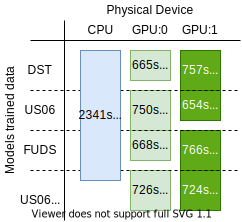
\includegraphics[width=0.60\linewidth]{II_Body/images/Accuracy_Compute.png}
    % \includesvg[width=\linewidth]{II_Body/images/Accuracy_Compute_10.svg}
    \caption{Accuracy computation using a single model trained on different proflies separately. The timing examples were taken from Model №5 computation process.}
    \label{fig:device_compute}
\end{figure}
\begin{table}[ht]
    \centering
    \caption{Model performance results across multiple devices..}
    \label{tab:speed}
    \begin{tabular}{c c c |c c c}
        \hline
        Structure                &Total params& flop/it & Coral TPU (ms) & R-Pi4 (ms)      & Android (ms) \\
        \hline
        1 $\times$ LSTM(500)     & 1,008,501  & 2.0G & 227.9$\pm$17.2 & 2021.6$\pm$164.9 & 4058.7$\pm$45.0 \\% 4048.0$\pm$69.0 \\   %FLOPs:2,018,005
        1 $\times$ GRU(560)      & 949,761    & 1.9G & 198.3$\pm$36.6 & 2104.2$\pm$109.6 & 3809.2$\pm$41.5 \\%3815.9$\pm$33.0 \\   %FLOPs:189,903
        LSTM(500) \& Atten
                                 & 1,361,881  & 3.2G & 206.9$\pm$32.9 & 2125.2$\pm$126.1 & 4711.2$\pm$51.0 \\%4711.8$\pm$41.5 \\ %FLOPs:3,222,344
%        2 $\times$ GRU(60)       & 33,762     & Unkn & ** & ** & \\
        1 $\times$ GRU(500)      & 758,001    & 1.5G & 140.8$\pm$24.7 & 1816.1$\pm$129.1 & 3227.5$\pm$37.5 \\%3241.7$\pm$32.5 \\  % FLOPs:1,516,503
        2 $\times$ LSTM(250)     & 504,201    & 1.1G & 102.2$\pm$16.3 & 1802.6$\pm$131.1 & 2494.4$\pm$34.0 \\%2454.4$\pm$33.0 \\   % FLOPs:1,109,409
%        1 $\times$ Layer \& Dense& 3,369      &     & 2.35$\pm$0.25  & 3.15$\pm$0.85 & 6.3*\\
        \hline
    \end{tabular}
\end{table}

\section{Conclusion} \label{sec:conclussion}
%* Summarise
%* -Testing approach
%* -Results
%* -Future work
%? Summarise key findings
%? - Accurate methods of developed to fit ML to SoC
%? - BEst training - Best model

%
%
The work has offered several implementations of Machine Learning algorithms for State of Charge estimation of A123 Lithium-Ion batteries.
Several Recursive Neural Network models were selected from already published based on the most common and promising structures and optimisers.
Five models were investigated, implemented, performance measured, and cross-evaluated using three drive cycles at five battery temperature ranges together from 20-50\textdegree{}.
Half a dozen thousand samples per profile of charge and discharge cycles were resampled to equal 1Hz rate and organised in 500 samples long matrices consisting of Voltage, Current, Temperature and corresponding charge percentage.
To adequately compare performance across models and comprehend the stochastic nature of Machine Learning a set of hyperparameters was predetermined through trial and error evaluation and multiple attempts of averaging.
By involving a learning rate scheduler and rollback technique to justify early stopping the speed of the training has been increased and the probability of model early overfill has been reduced.

%
%
After comparing 135 models of different sets of Layers and Neurons, the most accurate, lightweight and reasonable training time long ended up being 3 layers with 43 neurons per each.
Then, another 150 combinations of 5 methods models for 3 driving profiles ten times were processed through the same training, testing and performance measurement procedures, to conclude that a DST-based simple LSTM with Adam optimisers make the best self and others capturing model.
The next, which can closely match the same results, but with better self-capturing capabilities ended up being an LSTM with an Attention model.
While an Attention layer had a significant impact on capturing the complex driving profiles like FUDS, it failed to characterise the other two.
Both models were trained for relatively the same number of epochs, going through multiple attempts of learning rate reduction scheduler to achieve the lowest possible optimum.
Even though the error results were mostly commonly doubled from their already published equivalents, with the tripled amount of data and complexity of fitting both charge and discharge cycles, the increased error in prediction battery cycles remained below 5\% and line fitting accurately describes a State of Charge behaviour, especially at critical points of full charge and depletion.

%
%
Even though most models provided excellent results, they lacked the accuracy of time-series models, observed in similar scenarios.
The highest error regions were observed at the middle point of the charge, where the voltage of Lithium Ion batteries stays at 3.3V most of the time.
Being the SoC the function of current, that behaviour could indicate that Recurrent Neural Networks are tended to put more weight on the voltage feature instead.
While Model \#1 was chosen to be the best model for generalisation driving behaviour, it has little room for improvement, whereas Model \#3 with its extension to the structure may prove as a vital starting point for the next research iteration of charge prediction models, utilising output feature as an input, like time-series models tend to do in the other scenarios.

\section{TOBE READAPTED TO MDPI specs}
\section{Acknowledgements}\label{sec:acknowledgements}
The research was undertaken through funding from the Automotive Engineering Graduate Program (AEGP) in cooperation with the Queensland government and Prohelion industry partner.
All models evaluation has been performed through the help of the QUT HDR research and technical staff, who arranged access to the Hight Performance Machine (HPC Lyra) for the extensive initial computations.
The research has been conducted in cooperation with Mr Sam Haines, who performed a similar investigation on a similar dataset using Kalman filters and its' branches.
In addition, both Sam and I owe our progress to our Principal and Associate supervisors, Associate Professors David Holmes and Geoff Walker, who have been following our progress through the entire research.
Finally, we gratefully acknowledge the original developers of the Machine Learning framework Tensorflow from Google, who wrote detailed guides and documentation for all necessary tools used throughout the investigation.
%It is worth acknowledging the input from Dr Olga, Dr Mahsa and Pr Lovell who showed a practical interesr in the research and ... contribtution.

Manuscript received Month xx, 2xxx; revised Month xx, XXXX; accepted Month x, XXXX.
This work was supported in part by the Government of Australia under Automotive Engineering Graduate Program (AEGP) Grant.

Marat Sadykov, Sam Haines and A/Prof David Holmes are with the School of Mech., Medical \& Process Engineering,  Queensland University of Technology (QUT), Brisbane, QLD, 4000, Australia. (e-mail: d.holmes@qut.edu.au). 

Dr Mark Broadmeadow and A/Prof Geoff Walker are with the School of Electrical Engineering \& Robotics,  Queensland University of Technology (QUT), Brisbane, QLD, 4000, Australia. %(e-mail: mark.broadmeadow@qut.edu.au, geoffrey.walker@qut.edu.au)

%%%%%%%%%%%%%%%%%%%%%%%%%%%%%%%%%%%%%%%%%%
\vspace{6pt} 

%%%%%%%%%%%%%%%%%%%%%%%%%%%%%%%%%%%%%%%%%%
%% optional
%\supplementary{The following supporting information can be downloaded at:  \linksupplementary{s1}, Figure S1: title; Table S1: title; Video S1: title.}

% Only for the journal Methods and Protocols:
% If you wish to submit a video article, please do so with any other supplementary material.
% \supplementary{The following supporting information can be downloaded at: \linksupplementary{s1}, Figure S1: title; Table S1: title; Video S1: title. A supporting video article is available at doi: link.}

%%%%%%%%%%%%%%%%%%%%%%%%%%%%%%%%%%%%%%%%%%
\authorcontributions{
	For research articles with several authors, a short paragraph specifying their individual contributions must be provided. The following statements should be used ``Conceptualization, X.X. and Y.Y.; methodology, X.X.; software, X.X.; validation, X.X., Y.Y. and Z.Z.; formal analysis, X.X.; investigation, X.X.; resources, X.X.; data curation, X.X.; writing---original draft preparation, X.X.; writing---review and editing, X.X.; visualization, X.X.; supervision, X.X.; project administration, X.X.; funding acquisition, Y.Y. All authors have read and agreed to the published version of the manuscript.'', please turn to the  \href{http://img.mdpi.org/data/contributor-role-instruction.pdf}{CRediT taxonomy} for the term explanation. Authorship must be limited to those who have contributed substantially to the work~reported.
}

\funding{
    The research was funded by the Automotive Engineering Graduate Program (AEGP), grand number AEGP000036, from the Australian Government Department of Industry Science, Energy and Resources in cooperation with industry partner Prohelion.

    
    and  add ``The APC was funded by XXX''. Check carefully that the details given are accurate and use the standard spelling of funding agency names at \url{https://search.crossref.org/funding}, any errors may affect your future funding.
}

\institutionalreview{
    In this section, you should add the Institutional Review Board Statement and approval number, if relevant to your study. You might choose to exclude this statement if the study did not require ethical approval. Please note that the Editorial Office might ask you for further information. Please add “The study was conducted in accordance with the Declaration of Helsinki, and approved by the Institutional Review Board (or Ethics Committee) of NAME OF INSTITUTE (protocol code XXX and date of approval).” for studies involving humans. OR “The animal study protocol was approved by the Institutional Review Board (or Ethics Committee) of NAME OF INSTITUTE (protocol code XXX and date of approval).” for studies involving animals. OR “Ethical review and approval were waived for this study due to REASON (please provide a detailed justification).” OR “Not applicable” for studies not involving humans or animals.
}

\informedconsent{
    Any research article describing a study involving humans should contain this statement. Please add ``Informed consent was obtained from all subjects involved in the study.'' OR ``Patient consent was waived due to REASON (please provide a detailed justification).'' OR ``Not applicable'' for studies not involving humans. You might also choose to exclude this statement if the study did not involve humans.

    Written informed consent for publication must be obtained from participating patients who can be identified (including by the patients themselves). Please state ``Written informed consent has been obtained from the patient(s) to publish this paper'' if applicable.
}

\dataavailability{
    In this section, please provide details regarding where data supporting reported results can be found, including links to publicly archived datasets analyzed or generated during the study. Please refer to suggested Data Availability Statements in section ``MDPI Research Data Policies'' at \url{https://www.mdpi.com/ethics}. If the study did not report any data, you might add ``Not applicable'' here.
}

\acknowledgments{
    In this section you can acknowledge any support given which is not covered by the author contribution or funding sections. This may include administrative and technical support, or donations in kind (e.g., materials used for experiments).
}

\conflictsofinterest{
    The authors declare no conflict of interest.
    The funders had no role in the design of the study; in the collection, analyses, or interpretation of data; in the writing of the manuscript; or in the decision to publish the~results

    
    Authors must identify and declare any personal circumstances or interest that may be perceived as inappropriately influencing the representation or interpretation of reported research results. Any role of the funders in the design of the study; in the collection, analyses or interpretation of data; in the writing of the manuscript; or in the decision to publish the results must be declared in this section. If there is no role, please state ``The funders had no role in the design of the study; in the collection, analyses, or interpretation of data; in the writing of the manuscript; or in the decision to publish the~results''.
} 

%%%%%%%%%%%%%%%%%%%%%%%%%%%%%%%%%%%%%%%%%%
%% Optional
\sampleavailability{Samples of the compounds ... are available from the authors.}

%% Only for journal Encyclopedia
%\entrylink{The Link to this entry published on the encyclopedia platform.}

\abbreviations{Abbreviations}{
The following abbreviations are used in this manuscript:\\

\noindent 
\begin{tabular}{@{}ll}
    Adam & Adaptive Moment Estimation\\
    Adamax & Adaptive Moment Estimation based on the infinity norm\\
    EV & Electric Vehicle (EV)\\
    GRU & Gradient Recurrent Unit\\
    Li-Ion & Lithium-Ion battery\\
    LSTM & Long Short-Term Memory\\
    MDPI & Multidisciplinary Digital Publishing Institute\\
    Nadam & Nesterov Adaptive Moment Estimation\\
    RNNs & Recurrent Neural Networks\\
    RoAdam & Robust Online Adaptive Moment Estimation\\
    SoC & State of Charge\\
    SGDw/M & Stochastic Gradient Descent with Momentum\\
    TF & TensorFlow
    % DOAJ & Directory of open access journals\\
    % TLA & Three letter acronym\\
    % LD & Linear dichroism
\end{tabular}
}

%%%%%%%%%%%%%%%%%%%%%%%%%%%%%%%%%%%%%%%%%%
%% Optional
\appendixtitles{no} % Leave argument "no" if all appendix headings stay EMPTY (then no dot is printed after "Appendix A"). If the appendix sections contain a heading then change the argument to "yes".
\appendixstart
\appendix
\section[\appendixname~\thesection]{Robust Adam implementation} \label{app:RoAdam}
% \subsection[\appendixname~\thesubsection]{}
\input{../X-Appendix/AppendixE}
\clearpage
\section[\appendixname~\thesection]{Getting Number of Flops from TF2.4} \label{app:flops}
\input{../X-Appendix/AppendixF}
%%%%%%%%%%%%%%%%%%%%%%%%%%%%%%%%%%%%%%%%%%
\begin{adjustwidth}{-\extralength}{0cm}
%\printendnotes[custom] % Un-comment to print a list of endnotes

\reftitle{References}

% Please provide either the correct journal abbreviation (e.g. according to the “List of Title Word Abbreviations” http://www.issn.org/services/online-services/access-to-the-ltwa/) or the full name of the journal.
% Citations and References in Supplementary files are permitted provided that they also appear in the reference list here. 

%=====================================
% References, variant A: external bibliography
%=====================================
\bibliography{
    ../Z-References/References,
    I_Introduction/BibIntro,
    II_Body/BibRNN,
    II_Body/LSTM/BibLSTM,
    II_Body/GRU/BibGRU,
    II_Body/Optimisers/BibOpt.bib
}

% If authors have biography, please use the format below
%\section*{Short Biography of Authors}
%\bio
%{\raisebox{-0.35cm}{\includegraphics[width=3.5cm,height=5.3cm,clip,keepaspectratio]{Definitions/author1.pdf}}}
%{\textbf{Firstname Lastname} Biography of first author}
%
%\bio
%{\raisebox{-0.35cm}{\includegraphics[width=3.5cm,height=5.3cm,clip,keepaspectratio]{Definitions/author2.jpg}}}
%{\textbf{Firstname Lastname} Biography of second author}

% For the MDPI journals use author-date citation, please follow the formatting guidelines on http://www.mdpi.com/authors/references
% To cite two works by the same author: \citeauthor{ref-journal-1a} (\citeyear{ref-journal-1a}, \citeyear{ref-journal-1b}). This produces: Whittaker (1967, 1975)
% To cite two works by the same author with specific pages: \citeauthor{ref-journal-3a} (\citeyear{ref-journal-3a}, p. 328; \citeyear{ref-journal-3b}, p.475). This produces: Wong (1999, p. 328; 2000, p. 475)

%%%%%%%%%%%%%%%%%%%%%%%%%%%%%%%%%%%%%%%%%%
%% for journal Sci
%\reviewreports{\\
%Reviewer 1 comments and authors’ response\\
%Reviewer 2 comments and authors’ response\\
%Reviewer 3 comments and authors’ response
%}
%%%%%%%%%%%%%%%%%%%%%%%%%%%%%%%%%%%%%%%%%%
\end{adjustwidth}
\end{document}

